\documentclass[pdftex,fontsize=12pt,a4paper,numbers=noenddot]{scrreprt}
%
%Beinhaltet alle verwendeten Pakete
% Dateiformat 
\usepackage[utf8]{inputenc}

% Sprache
\usepackage[ngerman]{babel}

% Silbentrennung
\usepackage[T1]{fontenc}  

% Serifenlose Schrift wie Arial
\usepackage[scaled]{uarial}
\renewcommand*{\familydefault}{\sfdefault}

% Seitenränder etc
\usepackage[left=3cm,right=3cm,top=2cm,bottom=2cm,bindingoffset=0mm]{geometry}

% Bilder und Grafiken
\usepackage{graphicx}
\usepackage{wrapfig}

% Kopf- und Fußzeilen
\usepackage{footmisc}
\usepackage[automark]{scrpage2} 

% Aufzählungen, Tabellen, ...
\usepackage{enumitem}
\usepackage{longtable}
\usepackage{supertabular}
\usepackage{tabularx}
\usepackage{longtable}
\usepackage{colortbl}
\usepackage{multirow}

% Nummerierung von Abbildungen
\usepackage{chngcntr}
\counterwithin{figure}{section}
\counterwithin{table}{section} 

% Schriftsatz
\usepackage{textcomp}
\usepackage{float}

%Abkürzungsverzeichnis
\usepackage{acronym}

% Hyperlinks in der PDF
\usepackage[colorlinks, linkcolor=black]{hyperref}
\usepackage{url}

\usepackage{pdflscape}
\usepackage{pdfpages}
% Dient zur Konfiguration von Layout und LaTeX
% Befehle zur Ausgabe von Tactical Training Team
\newcommand{\TTT}{Tactical Training Team}

% Zeilenabstand
\linespread{1.15}
\setlength{\parindent}{0pt} 

%Seitenränder
\geometry{
	left=30mm,
	right=20mm,
	top=30mm,
	bottom=30mm,
}

% Verzeichnisebenen Bilder und Tabellen
\counterwithin{figure}{section}
\counterwithin{table}{section} 

% Absand Aufzählung
\setlist[1]{itemsep=0pt}

% Farben
\usepackage{xcolor}
\definecolor{blue}{RGB}{0,0,120}
\definecolor{green}{RGB}{0,153,0}
\definecolor{backcolor}{rgb}{0.9,0.9,0.9}
\definecolor{yellow}{RGB}{255,210,0}
\definecolor{gold}{RGB}{218,165,32}
\definecolor{DarkOrchid}{RGB}{92,30,123}

% Url-Einstellungen
\hypersetup{%
	hidelinks,
	pdfauthor={\TTT}
}

% Einstellungen Kopf- und Fußzeile
\pagestyle{empty}
\clearscrheadfoot{}
\ofoot[]{\textbf{\vrule}\,\pagemark}
%\ihead[]{Tactical Training Team}
%\ohead[]{\headmark}
\chead[]{
\includegraphics[width=1.05\textwidth]{../img/header}}
\addtolength{\headheight}{10mm}
\addtolength{\footskip}{-10mm}
%\setheadsepline[\textwidth]{1pt}[\color{800000}]

% Ebenen Nummerierungen
\setcounter{secnumdepth}{4} %Nummerierungsebenen
\setcounter{tocdepth}{1}   %Ebenen Inhaltsverzeichnis

%Neuer Splatentyp für Tabellen (dient dazu, dass die erste Splate zentiert werden kann)
\newcolumntype{C}[1]{>{\centering\arraybackslash}m{#1}}
%linksbündiger Spaltentyp
\newcolumntype{P}[1]{>{\raggedright\arraybackslash}p{#1}}

%Eigenen Befehl für Newline definieren
\newcommand{\nl}{\newline}

%Autoref in Schreibmaschinenschrift
%\let\oldautoref\autoref
%\renewcommand{\autoref}[1]{\texttt{\oldautoref{#1}}}

%Nameref in Schreibmaschinenschrift und mit >> <<
\makeatletter
\shorthandon{"}
\AtBeginDocument{%
	\LetLtxMacro\oldnameref\nameref
	\DeclareRobustCommand*{\nameref}{%
		\@ifstar{\my@nameref*}{\my@nameref{}}%
	}%
	\newcommand*{\my@nameref}[2]{%
		\texttt{>>\oldnameref#1{#2}<<}%
	}%
}
\shorthandoff{"}
\makeatother

\renewcommand*{\familydefault}{\sfdefault}	
%\renewcommand*\chapterheadstartvskip {%
%	\vspace*{1\baselineskip plus .1\baselineskip minus .067\baselineskip}}

\begin{document}


\pagenumbering{gobble} %Seiten nicht mitzählen
%TODO: Grafisch Überarbeiten
\author{Tactical Training Team}
\begin{titlepage}
	\sffamily
	\begin{tabular}{|l>{\raggedright\hspace{0pt}\arraybackslash}p{0.9\linewidth}}
		& \\
		& \Large\textbf{Tactical Training Team}\\[\baselineskip]
		& \Huge\textbf{TTT Handbuch}\\
		& \\
		& \large\today\\
		& \\
	\end{tabular}
	\pagebreak
	\begin{center}
			
\includegraphics[width=\textwidth]{./img/TTTitelbild.png}
	\end{center}
\end{titlepage}

\newpage
\pagenumbering{roman} %ab hier werden römischen Seiten als Seitenzahlen mitgezählt

\tableofcontents % Inhaltsverzeichnis

\newpage
\pagenumbering{arabic} %ab hier werden Seiten als Seitenzahlen mitgezählt
\pagestyle{scrheadings}
\renewcommand{\chapterpagestyle}{scrheadings}
\chapter*{Vorwort}
\addcontentsline{toc}{chapter}{Vorwort} 
\subsection*{Über dieses Dokument}
%\addcontentsline{toc}{subsection}{Über dieses Dokument} 
	Entstanden aus dem ursprünglichen, kompakten Leitfaden zur Allgemeinen Grundausbildung im \ac{TTT} soll dieses Dokument sowohl Grünschnäbeln als auch Alten Hasen zum Erlernen und Festigen aller relevanten theoretischen Grundlagen des taktischen Spiels im \ac{TTT} dienen. Es ist Leitfaden, Referenzwerk und Messlatte in einem Dokument vereint. Wie jedes Schriftstück zur Ausbildung sollte es \textit{aktiv} gelesen werden: der Leserin oder der Leser sollte über die vermittelten Inhalte nachdenken, sie hinterfragen, diskutieren wo nötig und gewissenhaft einprägen.\\
	Dieses Dokument lebt, es wird weiterentwickelt, überarbeitet, erweitert, gekürzt -- Anmerkungen, Vorschläge und Rückmeldungen konstruktiver Art werden nicht nur gewünscht, sondern gefordert. Ein hoher Standard im Spiel beginnt mit einem hohen Standard und Anspruch an alle Unterlagen, und jeder Spieler im \ac{TTT} ist nicht nur ständigen Verbesserung und Erweiterung seiner eigenen Fähigkeiten verpflichtet, sondern auch zur Verbesserung und Erweiterung des vermittelten Wissens. Ein aufmerksamer, geübter Schütze mag den Ausgang eines Feuerkampfs für sich entscheiden -- der virtuelle Krieg wird jedoch durch Strategie, Taktik und das Wissen um das \textit{WIE} entschieden, das aus den Erfahrungen von Fehlschlägen und Triumphen herrührt. Der erste Schritt den du, lieber Leser, auf dem Weg zu einem erfolgreichen Spieler im \emph{[\ac{TTT}]} leisten musst, ist über diese Aussage zu meditieren und sie zu verstehen.\\

\textit{Train hard, play smart!}

\newpage
\subsection*{Die Grundsätze des TTT}
\label{sec:Grundsaetze}
%\addcontentsline{toc}{subsection}{Die Grundsätze des TTT} 
	\begin{itemize}
		\item Das [TTT] stellt das Training in den Mittelpunkt
		\item Das [TTT] spielt auf höchstem taktischen Niveau
		\item Das [TTT] orientiert sich in seiner Spielweise und Organisation an Kommando-Teams
		\item Das [TTT] pflegt und lebt das Battle Buddy System
		\item Das [TTT] lässt im Spiel keinen Kamerad zurück, jedem Notruf wird Folge geleistet
		\item Das [TTT] ist eine offene Community -- jeder kann am Training oder den Events grundsätzlich teilnehmen
		\item Die [TTT] Community wird geführt wie ein aktives, ergebnisorientiertes Unternehmen -- die Stammspieler sind das wichtigste Kapital	
	\end{itemize}

\part*{ATCHUNG hierbei handelt es sich um eine BETA-Version, dementsprechend können Abweichungen zu Training und Ensteigerevent existieren}
\part{Truppenordnung \& Basisentnisse}
%Truppengattungen
\chapter{Truppenordnung}
In diesem Abschnitt werden die einzelnen Strukturelemente und die Organisation des \ac{TTT} während einer typischen Mission erklärt.\\
Die hier vorgestellten Strukturen basieren dabei auf der im Laufe der Zeit gesammelten Erfahrung, was in ArmA funktioniert und was nicht und sind verpflichtende Vorgabe für jeden Missionsbauer. Ausnahmen von diesen Strukturen müssen vorher angefragt und genehmigt werden.\\
Da im \ac{TTT} sowohl deutsche als auch amerikanische Strukturen benutzt werden, werden die amerikanischen Namen jeweils in Klammern zusätzlich zu den deutschen Namen genannt.

\section{\acf{OPL} / \acf{HQ}}
\begin{wrapfigure}{r}{0.35\textwidth}
	%\vspace{-15pt}
	\centering 
	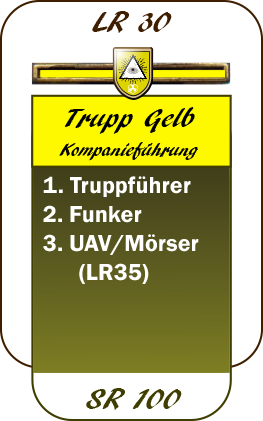
\includegraphics[width=0.3\textwidth]{../img/truppenordnung/opl/opl}
	%\caption{Beispiel einer \ac{OPL}}
	%\vspace{-30pt}
\end{wrapfigure}	

Die \ac{OPL} ist die höchste Instanz innerhalb einer Mission. Sie hat den Oberbefehl über alle Einheiten inne, koordiniert das allgemeine Vorgehen innerhalb der Mission und verwaltet die Zuordnung der unterstützenden Einheiten zu den kämpfenden Einheiten. Sie kommuniziert grundsätzlich nur über die Long-Range mit ihren untergeordneten Einheiten.\vspace{12pt}\\

Die \ac{OPL} ist folgendermaßen aufgebaut:
\begin{itemize}
	\item Operationsleiter\,/\,\acs{OPL} (\acf{CO}): Der Oberbefehlshaber der Mission. Er gibt die Befehle und erstellt "den großen Plan".
	\item stellv. \ac{OPL} (\acf{XO}): Unterstützt den \ac{OPL} bei seinen Aufgaben, typischerweise beim Funken mit den untergeordneten Trupps. Kann jedoch auch alle weiteren Aufgaben übernehmen, die ihm der \ac{OPL} überträgt -- er ist Mädchen für alles. Bewährt hat sich das Prinzip, dass der \ac{OPL} den eingehenden Funk übernimmt (Anfragen von anderen Trupps) und der stellv. \ac{OPL} den ausgehenden Funk (Abfragen von Statusberichten, Übermittlung von neuen Befehlen).
\end{itemize}
Ergänzt werden kann die \ac{OPL} durch maximal 4 Spieler, welche folgende Rollen einnehmen können:
\begin{itemize}
	\item Funker (\acf{RO}): ein zusätzlicher Funker, um die \ac{OPL} zu unterstützen, kann auf eine Spezialrolle beschränkt sein und für diese eine eigene LR-Frequenz bekommen (so kann es z.\,B. bei einer Mission mit vielen Lufteinheiten sinnvoll sein, jemanden zu haben, der sich auf einer eigenen Frequenz nur um die Koordination der Lufteinheiten um das Flugfeld kümmert und zentraler Ansprechpartner aller Lufteinheiten für Start-\,/\,Landemanöver ist)
	\item Aufklärungsoffizier (\acf{IO}): Sammelt alle verfügbaren, relevanten Daten und leitet diese gegebenenfalls an andere Trupps weiter. Hat meistens eine eigene, "große" Drohne (Greyhawk\,/\,Global Hawk) zur Feindaufklärung.
	\item freie Rolle (maximal einmal): je nach Mission kann es sinnvoll sein, dem \ac{OPL} einen Sanitäter, einen Nahsicherer, einen Fahrer o.\,Ä. zur Seite zu stellen
\end{itemize}
Je nach Größe und Struktur der Mission kann die \ac{OPL} identisch sein mit
\begin{itemize}
	\item der Sektionsführung, falls die Truppstruktur der Mission nur aus einer Sektion besteht
	\item der Zugführung, falls die Truppstruktur der Mission nur aus einem Zug besteht (egal ob Infanteriezug, Panzerzug oder mechanisierte Infanterie). Dies ist die einzige Ausnahme, in der die \ac{OPL} per Short-Range statt Long-Range mit ihren untergeordneten Einheiten kommuniziert.
\end{itemize}
Die OPL hält typischerweise einen sehr großen Abstand zu ihren Truppen - oft bleibt sie auch durchgehend in der Basis.

\section{Sektionsführung / Platoon Lead (PLT)}
\begin{wrapfigure}{r}{0.35\textwidth}
	\vspace{-20pt}
	\centering 
	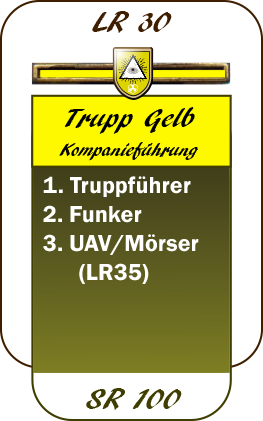
\includegraphics[width=0.3\textwidth]{../img/truppenordnung/sektionsfuehrung/sektionsfuehrung}
	%\caption{Beispiel einer Sektionsführung}
	\vspace{-5pt}
\end{wrapfigure}	
Die Sektionsführung ist ein Bindeglied zwischen OPL und Zugführung, um die OPL zu entlasten. Einer Sektionsführung sind mindestens zwei, maximal vier Züge unterstellt. Ab drei Zügen in einer Mission ist die Sektionsführung zwingend erforderlich, darunter optional.
\par\medskip
Die Sektionsführung ist folgendermaßen aufgebaut:
\begin{itemize}
	\item Sektionsführer\,/\,Platoon Lead (PLT): Er leitet die ihm untergeordneten Züge. Kommuniziert wird über Long-Range - entweder über die individuellen Frequenzen der einzelnen Züge oder über die Task-Force-Frequenz (siehe nächstes Kapitel).
	\item Funker / Radio Operator (RO): Übernimmt die Kommunikation zur OPL und anderen Einheiten.
\end{itemize}
Ergänzt werden kann die Sektionsführung bei Bedarf durch:
\begin{itemize}
	\setlength\itemsep{0em}
	\item einen Gefechtssanitäter\,/\,Combat Medic (CM) zur Versorgung im Feld.
	\item einen Fahrzeugführer\,/\,Nahsicherer zur selbstständigen Verlegung
\end{itemize} 
Die Sektionsführung befindet sich typischerweise etwas weiter entfernt hinter den ihr unterstellten Zügen.

\section{Zugführung / Squadlead (SQL)}
\begin{wrapfigure}{r}{0.4\textwidth}
	\centering 
	\vspace{-20pt}
	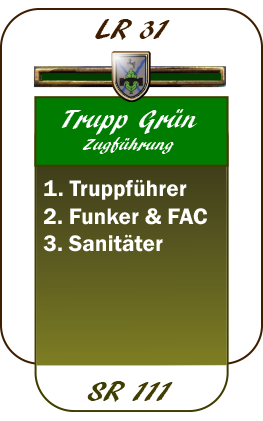
\includegraphics[width=0.3\textwidth]{./img/truppenordnung/zugfuehrung/zugfuehrung}
	%\caption{Beispiel eines \aclp{SQL}}
	\vspace{-50pt}
\end{wrapfigure}
Die Zugführung ist das Führungselement der Infanterie und Bindeglied zu den anderen Trupps. Einer Zugführung unterstellt sind typischerweise zwei, maximal drei Infanterietrupps, des weiteren kann ein Zug durch maximal einen Spezialtrupp mit klarer Aufgabenstellung unterstützt werden. Die Kommunikation zwischen dem Zugführer und der ihm untergeordneten Trupps erfolgt über Short-Range ohne Funkprotokoll über den sogenannten Zugkanal, die Kommunikation zu anderen Trupps über Long-Range.\\

Eine Zugführung besteht aus ein bis drei Spielern:
\begin{itemize}
	\item Zugführer\,/\,Squadlead (SQL)): Er befehligt die ihm untergeordneten Trupps. Ist kein Funker in der Zugführung vorhanden, übernimmt er auch die LR"=Kommunikation zu anderen Einheiten, in diesem Fall fällt jedoch die interne SR"=Truppfrequenz weg und der Zugfunk wird zum Standardfunk des Zugführers.
	\item Funker\,/\,Radio Operator (RO): Übernimmt die Kommunikation zu anderen Einheiten, damit der Zugführer sich auf die Führung seiner Truppen konzentrieren kann. Optional, wird jedoch dringend empfohlen.
	\item Gefechtssanitäter\,/\,Combat Medic (CM): Sanitäter für die Erstversorgung und Organisation der Verwundeten im Feld. Optional.
\end{itemize}
Sollten mehrere Züge im Verbund arbeiten, so einigen sich die Funker dieser Züge im Vorhinein auf eine sogenannte Task"=Force"=Frequenz, die sie sich auf der Additional"=Long"=Range einrichten und über die sie direkt ohne Funkprotokoll miteinander kommunizieren können (ähnlich wie der Zugkanal).\\
Die Zugführung sollte immer in Sichtweite der ihr unterstellten Trupps bleiben und sich maximal 200m bis 300m von ihnen entfernen, optimalerweise jedoch so nah wie möglich an ihren Truppen sein.
\section{Infanterietrupp / Fireteam (FT)}
\begin{wrapfigure}{R}{0.35\textwidth}
	\vspace{-50pt}
	\centering 
	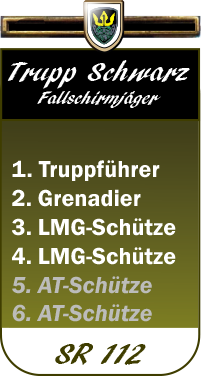
\includegraphics[width=0.2\textwidth]{../img/truppenordnung/infanterie/infanterie}
	%\caption{Beispiel eines Infantrietrupps}
	\vspace{-90pt}
\end{wrapfigure}
Die Infanterie bildet den Kernbestandteil vieler Missionen. Ein Infanterietrupp ist immer Teil eines Zuges und besteht aus 4 oder 6 Mann. Mögliche Positionen innerhalb eines Infanterietrupps sind:
\vspace{3.5cm}
\begin{longtable}{@{}P{0.4\textwidth}P{0.4\textwidth}@{}}
	\toprule
	Deutsche Bezeichnung & Englische Bezeichnung\\
	\midrule
	Truppführer (TF) & Fireteam Leader (FTL)\\
	Grenadier (GRE) & \\
	Leichter MG-Schütze (LMG) & Automatic Rifleman (AR)\\
	Mittlerer MG-Schütze & Medium Machine Gunner (MMG) \\
	MG-Assistent & Assistant Machine Gunner (AMG)\footnote{notwendig für MMG}\\ 
	Leichter Panzerabwehrschütze & Light Anti Tank (LAT)\\
	Schwerer Panzerabwehrschütze & Heavy Anti Tank (HAT)\\
	Panzerabwehr-Assistent & Assistant Anti Tank (AAT)\footnote{notwendig für HAT}\\ 
	Luftabwehrschütze & Anti-Air (AA)\\
	Pionier & Pioneer (PIO)\\
	Gefechtssanitäter & Combat Medic (CM)\\
	Schütze & Rifleman (RI)\\			
	\bottomrule					
\end{longtable}


Auf eine sinnvolle Einteilung in Buddy"=Teams (z.\,B. bei Positionen, die einen Assistenten erfordern), ist hierbei zu achten.\\
Die Kommunikation erfolgt ausschließlich über Short-Range, der Truppführer schaltet sich über seine Additional-Short-Range auf den Zugkanal auf, um sich mit der Zugführung und den anderen Truppführern im Zug abzusprechen. Die Nummer 2 im Trupp kann sich ebenfalls auf den Zugfunk aufschalten, jedoch nur mithören und nicht funken -- es sei denn, der Truppführer fällt aus und die Nummer 2 übernimmt.

\section{Spezialtrupp}

\includegraphics[width=20mm]{../img/truppenordnung/spezialeinheiten/sf1}\quad

\includegraphics[width=20mm]{../img/truppenordnung/spezialeinheiten/sf2}\linebreak
Spezialtruppen sind infanteristische Einheiten bestehend aus zwei bis sechs Mann mit einem klaren Aufgabenschwerpunkt -- dies kann vom klassischen Zwei"=Mann"=Scharfschützenteam bis zum Sechs-Mann-Kampftauchertrupp gehen. Sie sind die flexibelsten Einheiten innerhalb des TTTs und können entweder autark arbeiten oder im Verbund mit einem anderen Trupp oder Zug. Pro Mission existieren maximal zwei autark operierende Spezialtruppen, im Verbund mit einem Zug maximal einer.\par
Kommunikation erfolgt über Long"=Range, beim Arbeiten im Verbund zusätzlich über die Additional"=Short"=Range (Zugfunk). Kämpfende Einheiten wie z.B. Kommandotrupps oder Kampftaucher, in denen der Truppführer viel Mikromanagement leisten und der Trupp in direkte Feuergefechte verwickelt wird, benötigen zwingend einen separaten Funker. In unterstützenden Einheiten wie z.B. Aufklärungsteams oder Mörserteams, die voraussichtlich nicht in direkte Feuergefechte verwickelt werden, kann (muss aber nicht) der Truppführer die Long"=Range"=Kommunikation mit übernehmen.\par
Mögliche Aufgabenschwerpunkte eines Spezialtrupps sind z.\,B.:
\begin{itemize}
	\setlength\itemsep{0em}
	\item JTAC-Team
	\item Aufklärungsteam (UAV)
	\item Autonome Kampfeinheit (UGV)
	\item Mörserteam
	\item schwere Feuerunterstützung (Schweres Maschinengewehr (HMG) / Granatmaschinengewehr (GMG))
	\item (schwere) Panzerabwehr / Flugabwehr (falls nicht bereits im Zug vorhanden)
	\item Pionier-Team (falls nicht bereits im Zug vorhanden)
	\item medizinische Versorgung/Unterstützung (falls kein MedEvac in der Mission vorhanden)
	\item Kommandokräfte (Infiltration)
	\item Scharfschützenteam
	\item Kampftaucher
\end{itemize}
Bei entsprechenden Rollen (schwere Waffen, Mörser, etc.) ist auf das Vorhandensein eines entsprechenden Assistenten zu achten.
\section{Logistik}

\includegraphics[width=20mm]{./img/truppenordnung/logistikMedevac/TrSilber}\\
Silber -- Bussard -- Stellt Fahrzeuge und Personal bereit, mit denen Transport und Logistik durchgeführt werden.
\section{MedEvac}

\includegraphics[width=20mm]{../img/truppenordnung/logistikMedevac/weiss}\linebreak
Weiß -- \acf{MedEvac} -- Unterstützt Operationen mit Versorgungs- und Transportkapazität für Verwundete.
\section{Close Air Support}

\includegraphics[width=20mm]{../img/truppenordnung/logistikMedevac/silber}\\
Silber -- Adler -- Stellt Fahrzeuge und Personal bereit,  Gefechtsunterstützung (\ac{CAS}) und Geleitschutz durchgeführt werden.
\section{Mechanisierte Infanterie}
Das Konzept der mechanisierten Infanterie befindet sich im Moment noch in Arbeit und wird in einer späteren Version des Handbuches hinzugefügt.
\section{Kampfpanzer}
Das Konzept der Kampfpanzer befindet sich im Moment noch in Arbeit und wird in einer späteren Version des Handbuches hinzugefügt.
\section{Artillerie}
Das Konzept der Artillerie befindet sich im Moment noch in Arbeit und wird in einer späteren Version des Handbuches hinzugefügt.

% Grundlagen
\chapter{Basiskenntnisse}
%TODO Kurze Beschreibung

\section{Formationen}
Um sich durch das Gelände zu bewegen verwendet man Formationen. Diese können für die Trupp von Vorteil sein oder gewisse Nachteile haben. Deshalb sollten sie jederzeit dem Gelände, sowie erwarteten oder bekannten Situationen angepasst werden. Die Formationen die im TTT Verwendung finden sind der \textit{Stack}, die \textit{Kolonne} und die \textit{Schützenkette}. 

\subsection{Der Stack}
Der Stack ist die Sammelformation vor dem Abmarsch und als Bewegungsformation beim Einstieg in Fahrzeuge. Zudem dient er als Formation für den direkten Zugriff in Räume (siehe CQB). %TODO REF CQB
Grundsätzlich wird der Stack in den klassischen (engen) <<Stack>> und <<Stack weit>> unterteilt. Beim <<Stack weit>> werden die Abstände lediglich erweitert.\par
\begin{figure}[h]
	\centering
	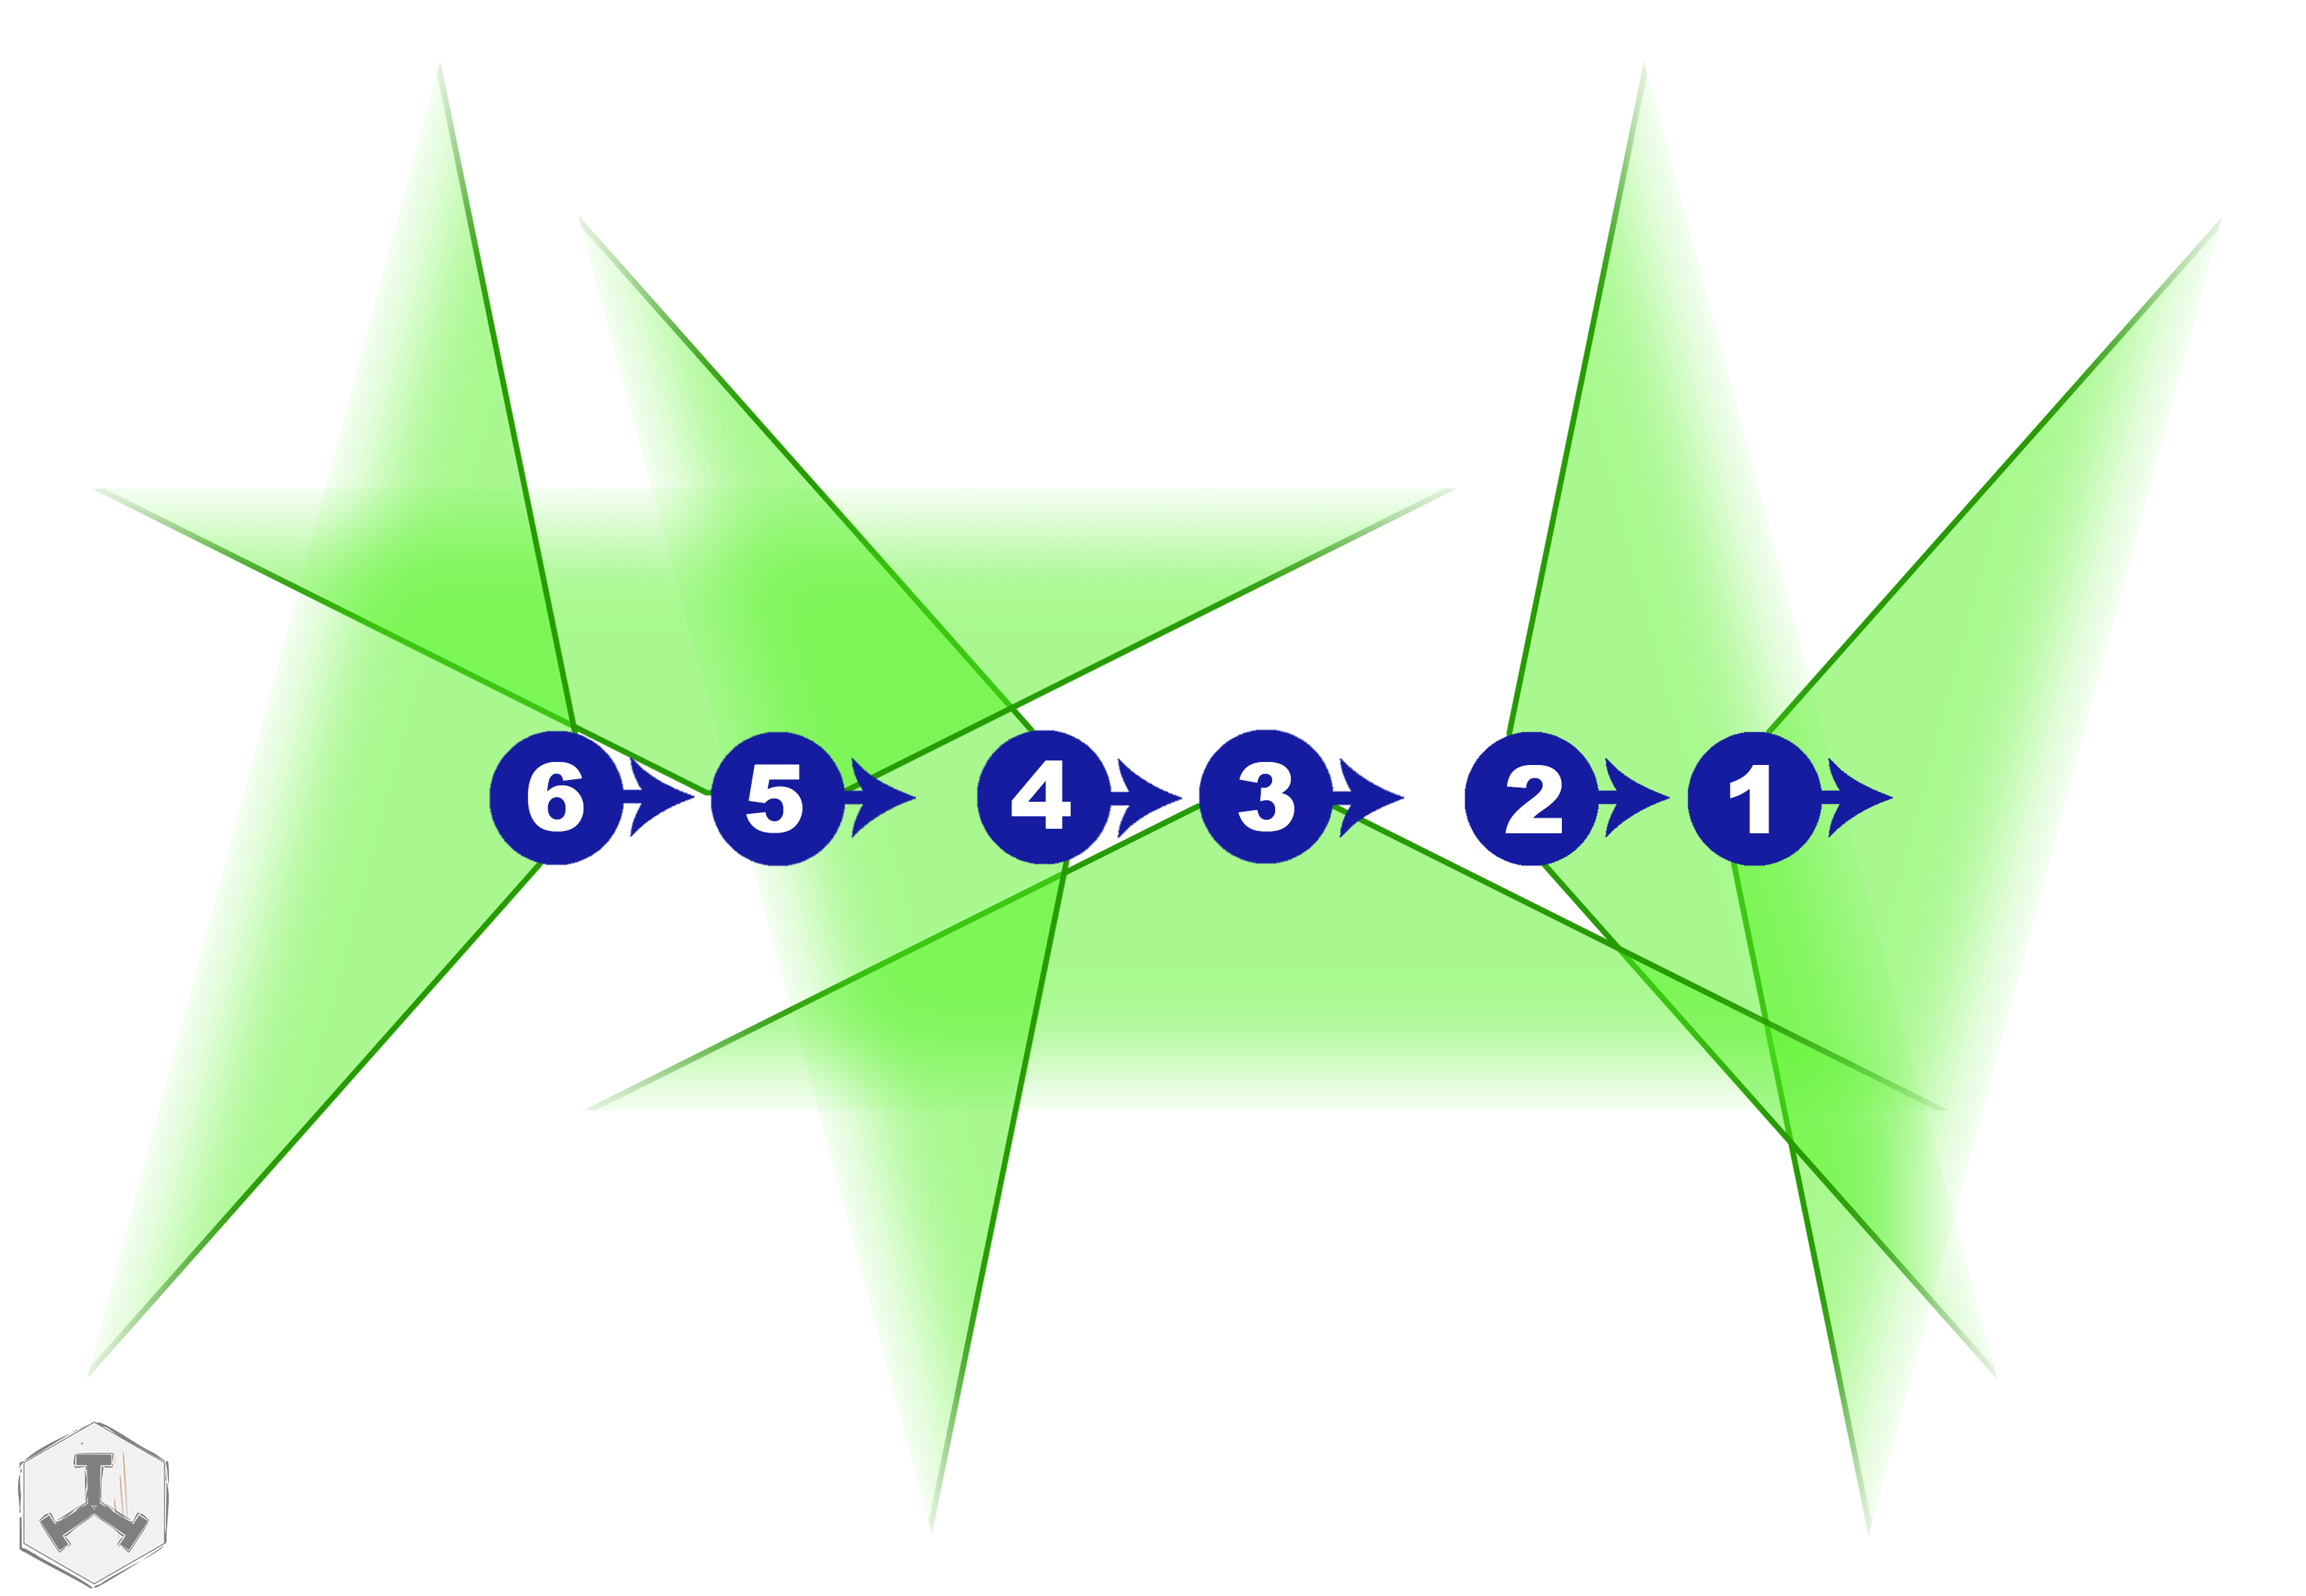
\includegraphics[width=0.7\linewidth]{../img/basic/formation/stack_6mann}
	\caption{Stack 6 Mann}
\end{figure}

\subsection{Die Kolonne}\label{Kolonne}
Die Kolonne dient als Formation im offenen Gelände und ist die Standardformation für den Marsch. Hierbei muss man zwischen einer Besonderheit im \ac{TTT} der Buddy"=Kolonne und der klassischen Kolonne unterscheiden. Die Buddy"=Kolonne garantiert, dass beispielsweise MG-Schütze und MG-Assistent immer zusammenbleiben. Zudem verringert sie die Ausfallzahl, da sich Buddies besser gegenseitig unterstützen können. Im Gegenzug ist die klassische Kolonne weniger anfällig für Sprengsätze und Beschuss. Die Abstände zwischen den Teams sollten etwa 20\,m betragen.
\begin{figure}[h]
	\centering
	\subfigure[Kolonne]{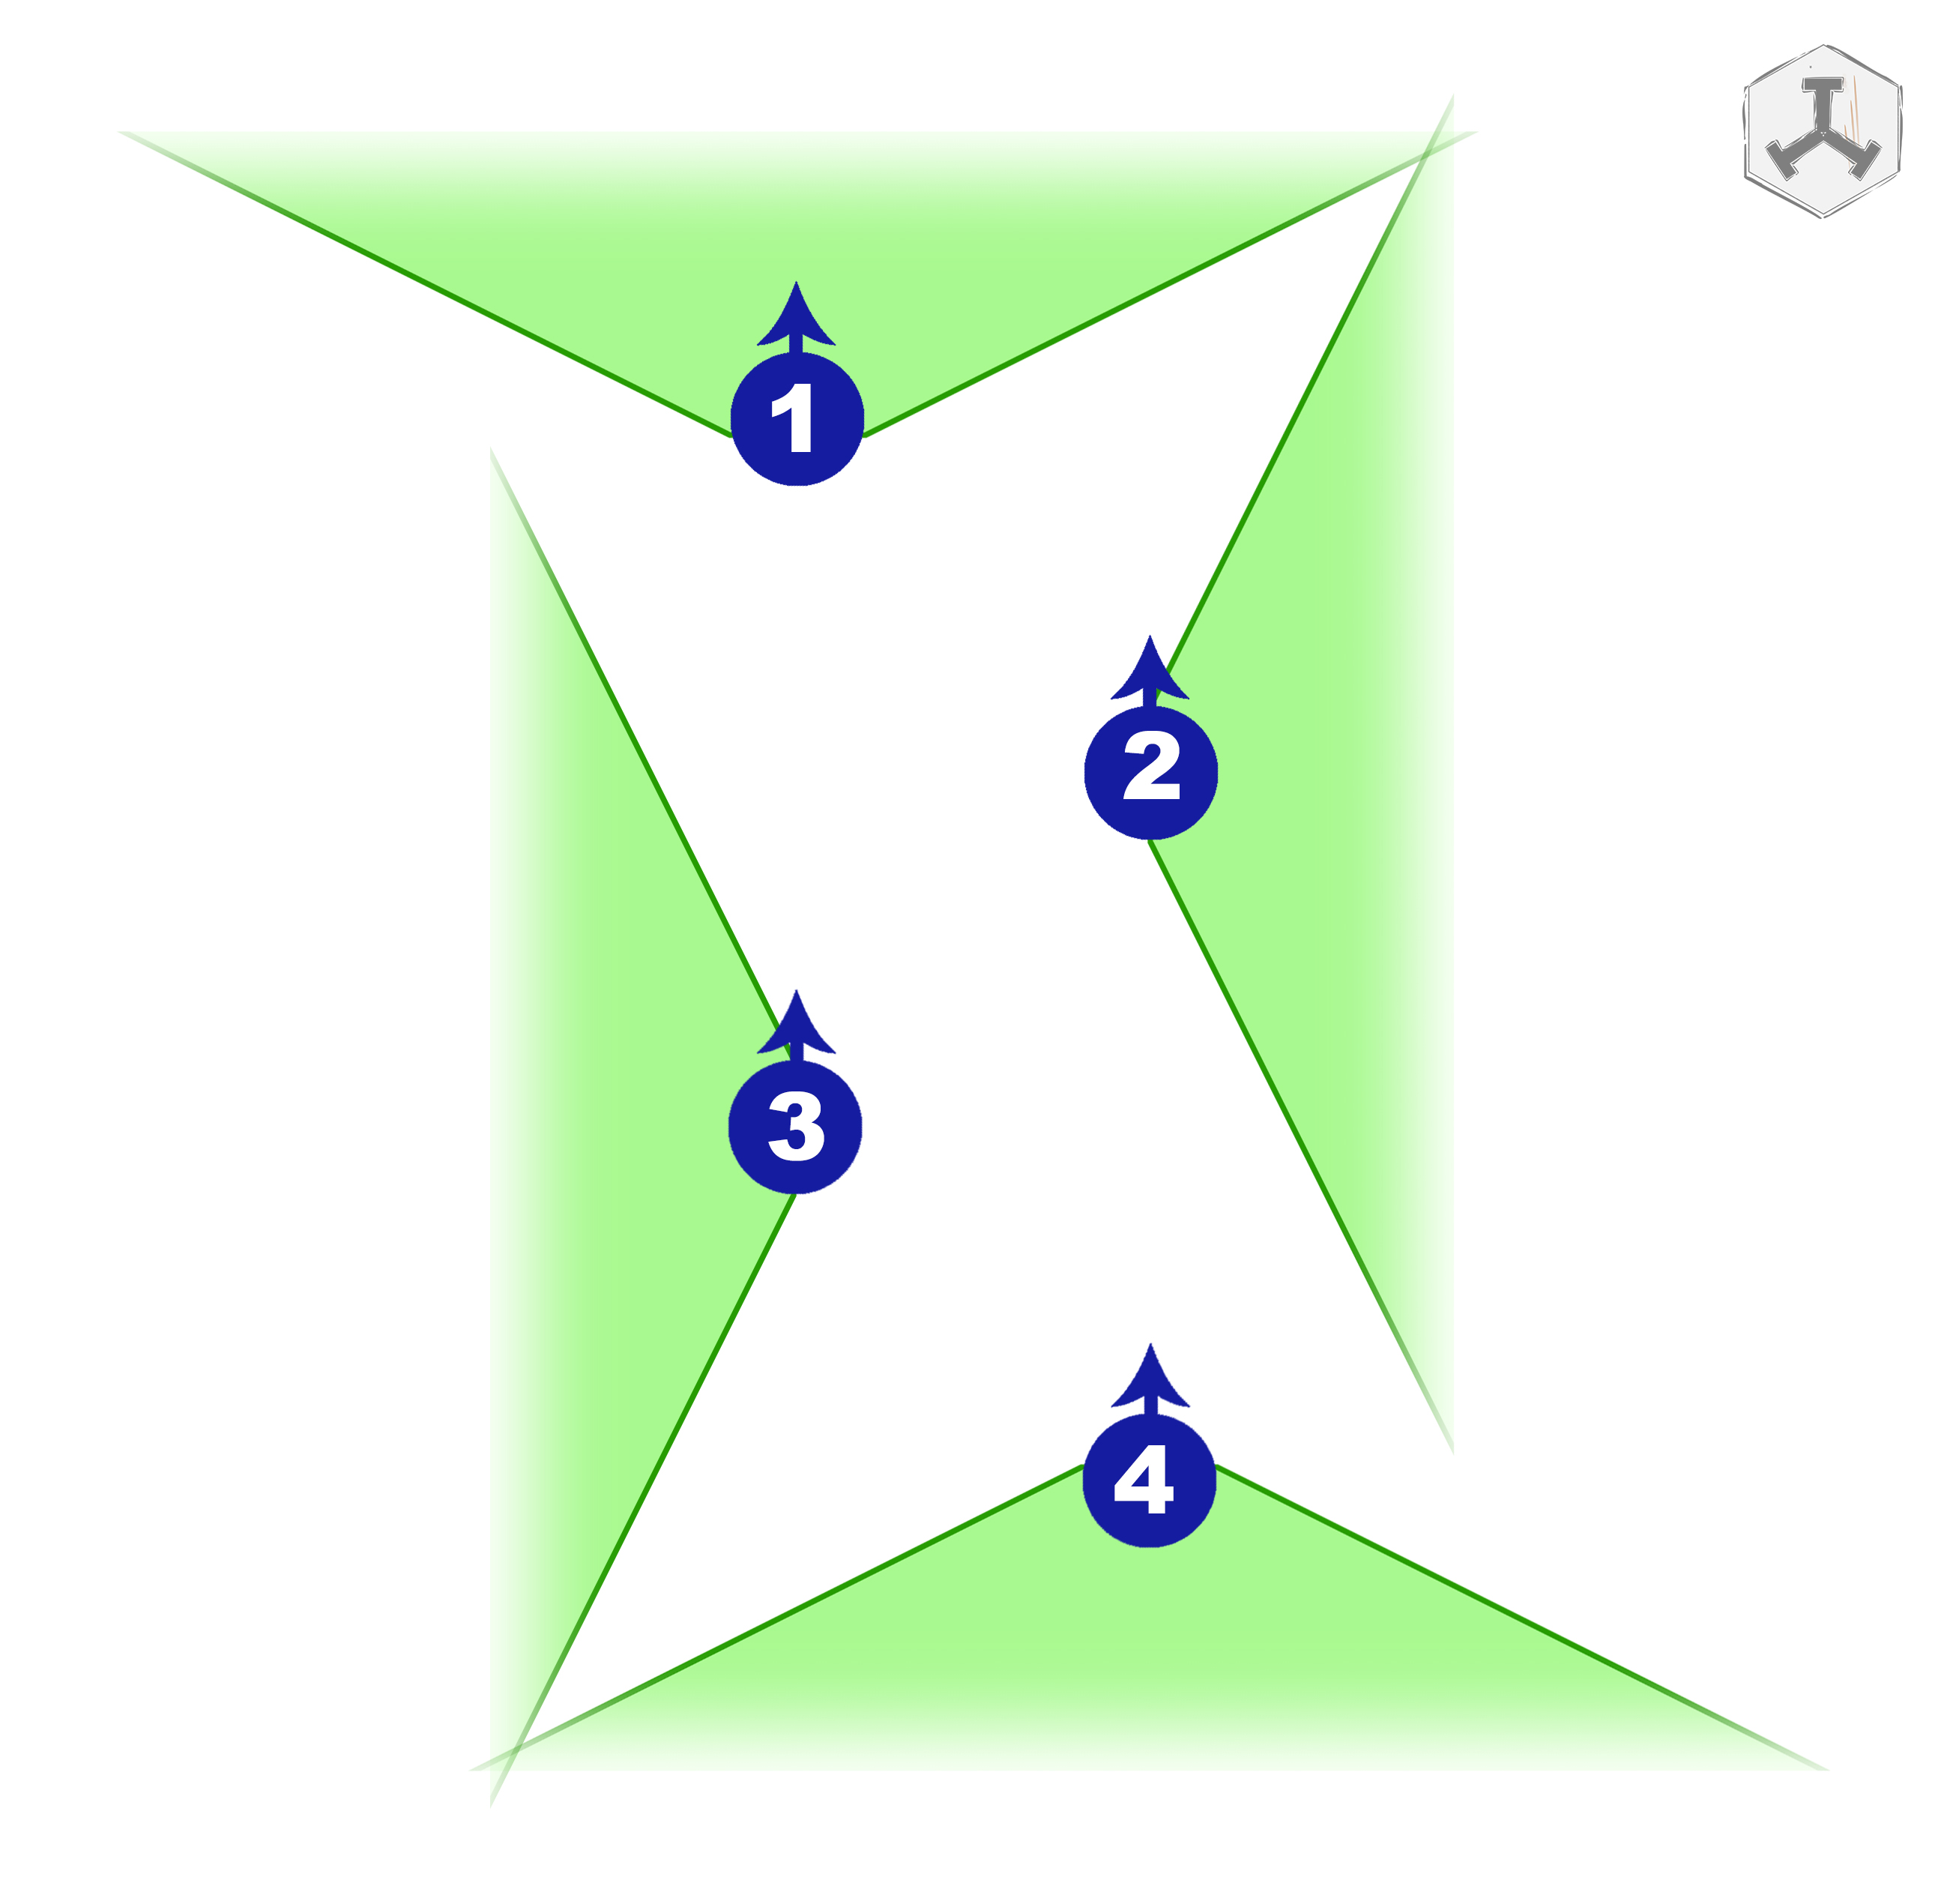
\includegraphics[width=0.49\linewidth]{../img/basic/formation/kolonne_4mann}}
	\subfigure[Buddy-Kolonne]{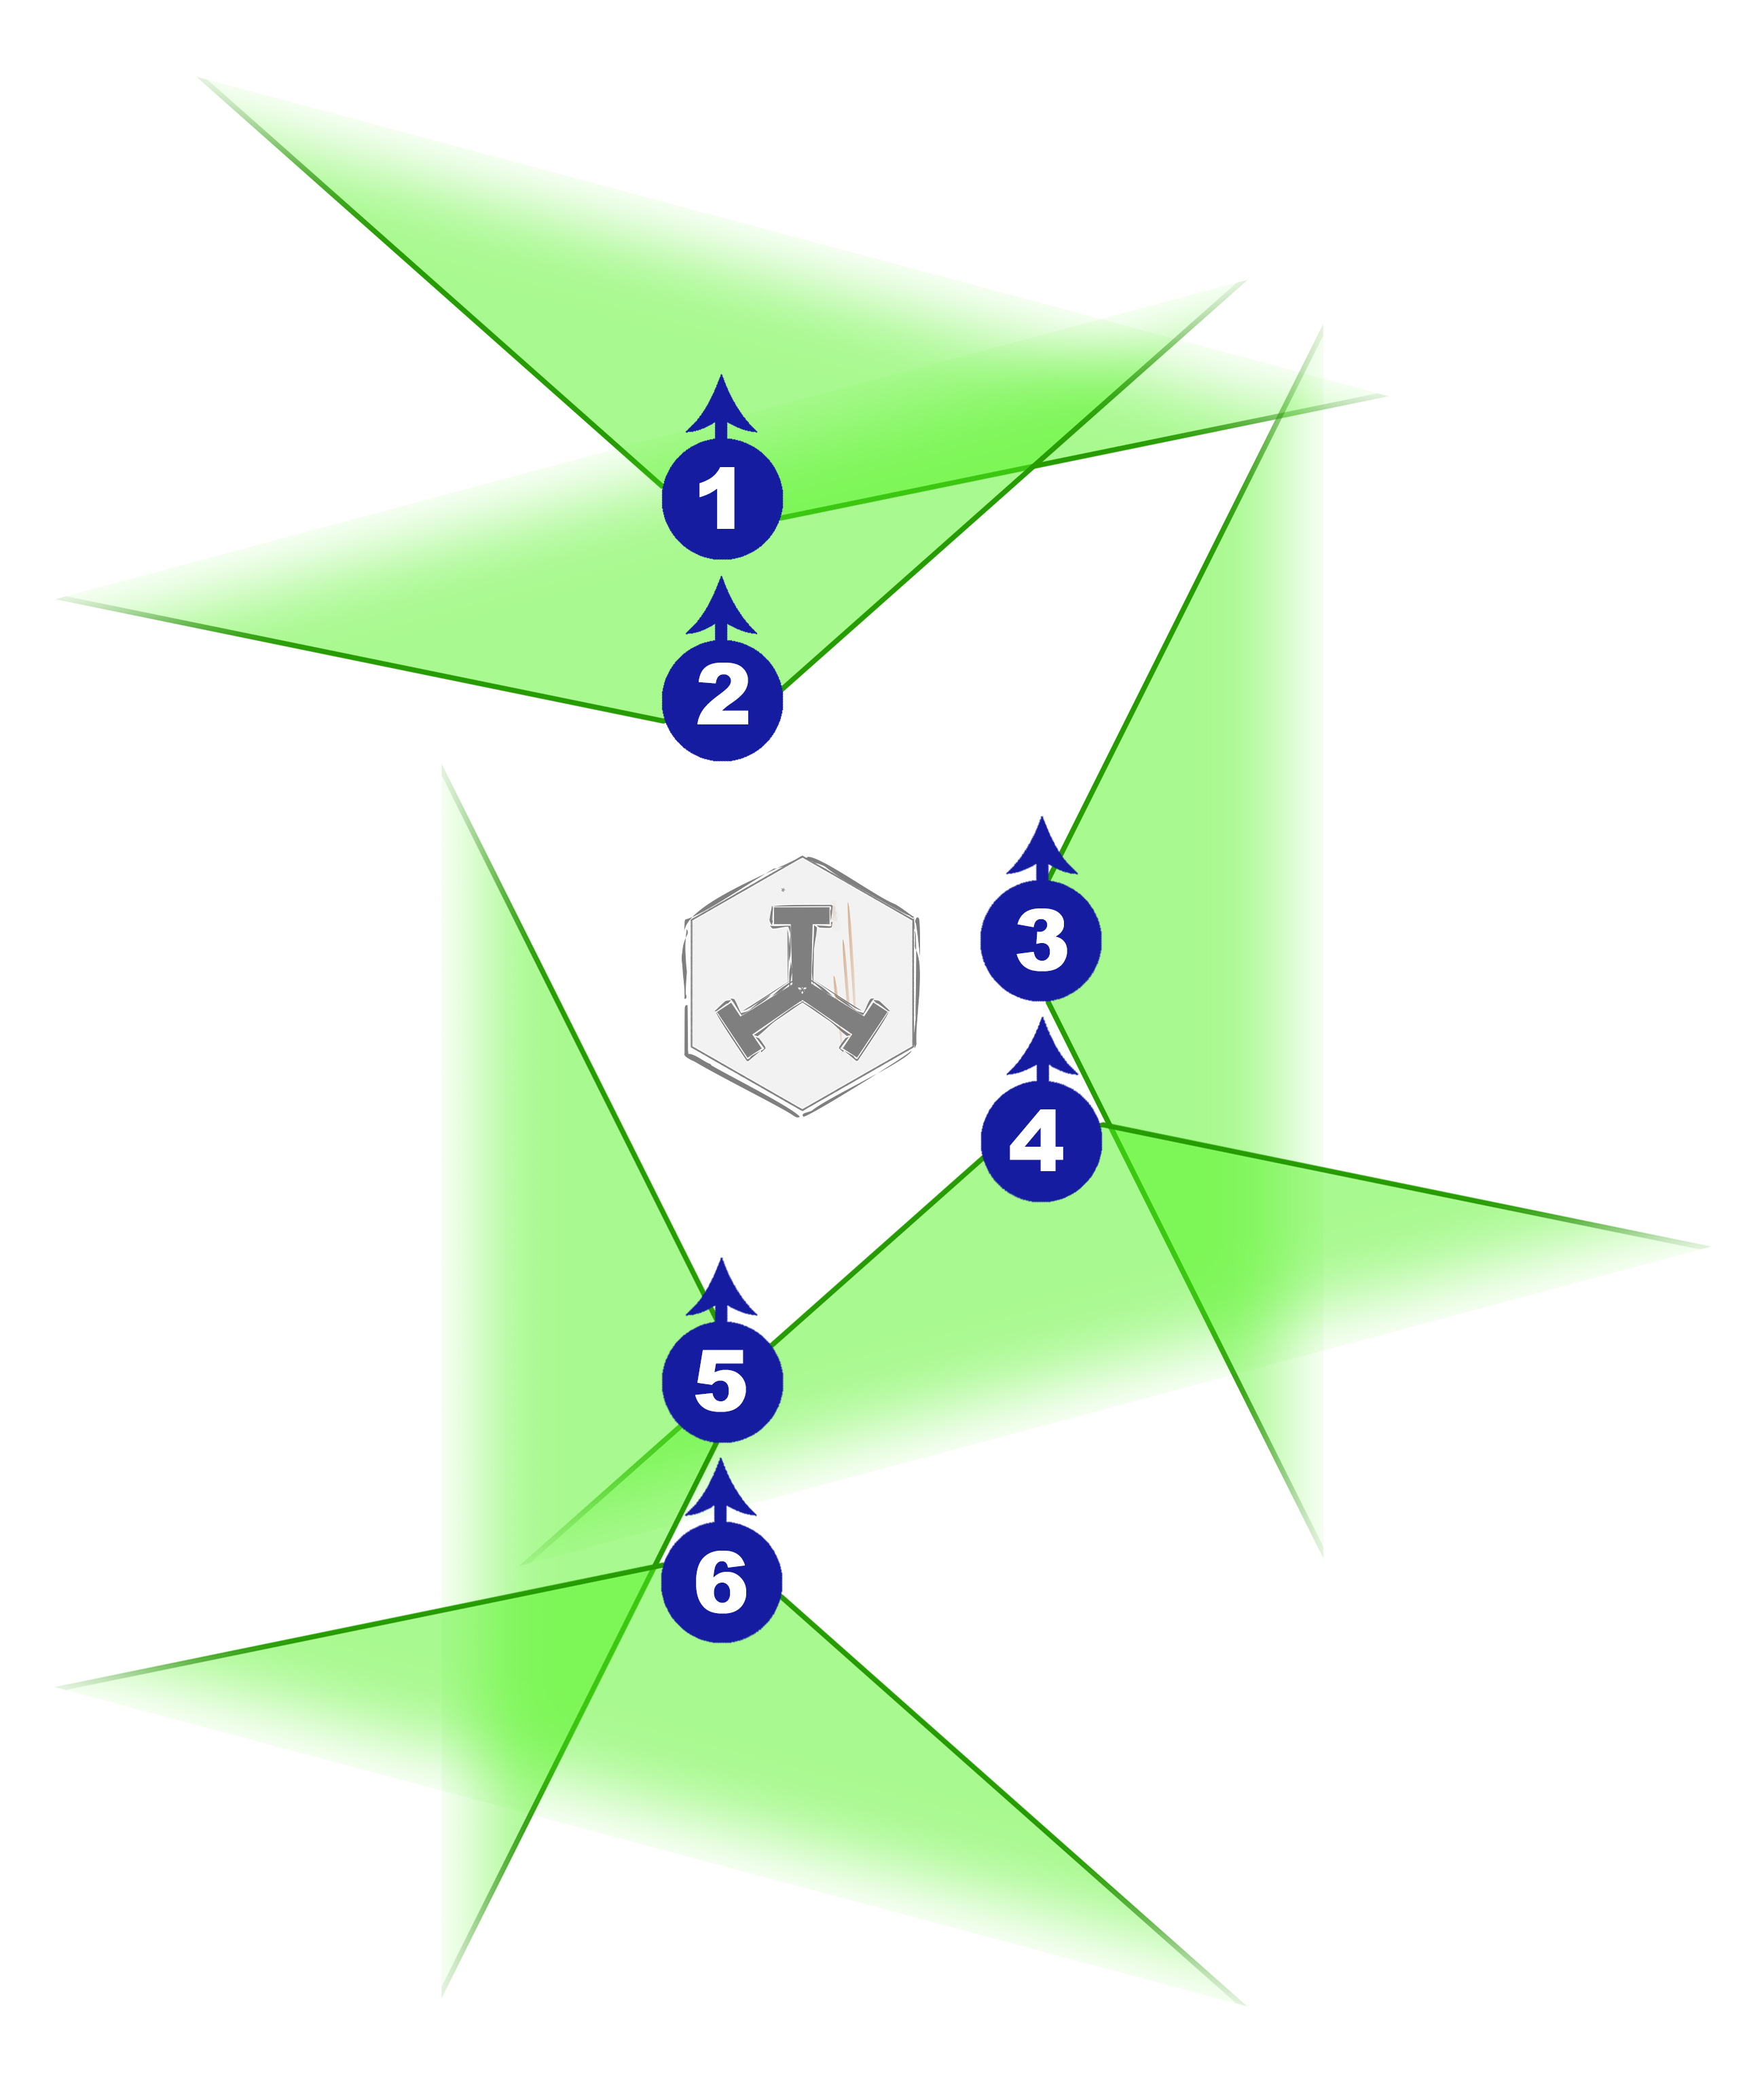
\includegraphics[width=0.49\linewidth]{../img/basic/formation/kolonne_6mann}}
	\label{fig:Kolonne}
\end{figure}

\subsection{Die Schützenkette}
Die Schützenkette dient zum Bezug einer Stellung, in Deckung an Mauern und -- in Ausnahmefällen! -- zum Anmarsch auf einen Feind. Sie bietet maximale Feuerkraft in vermuteter Feindrichtung, lässt jedoch die Flanken und den Rückraum ungesichert. Die Schützenkette kann durch entsprechende Flanken- und Rücksicherung effizienter gestaltet werden.
\begin{figure}[htbp]
	\centering
	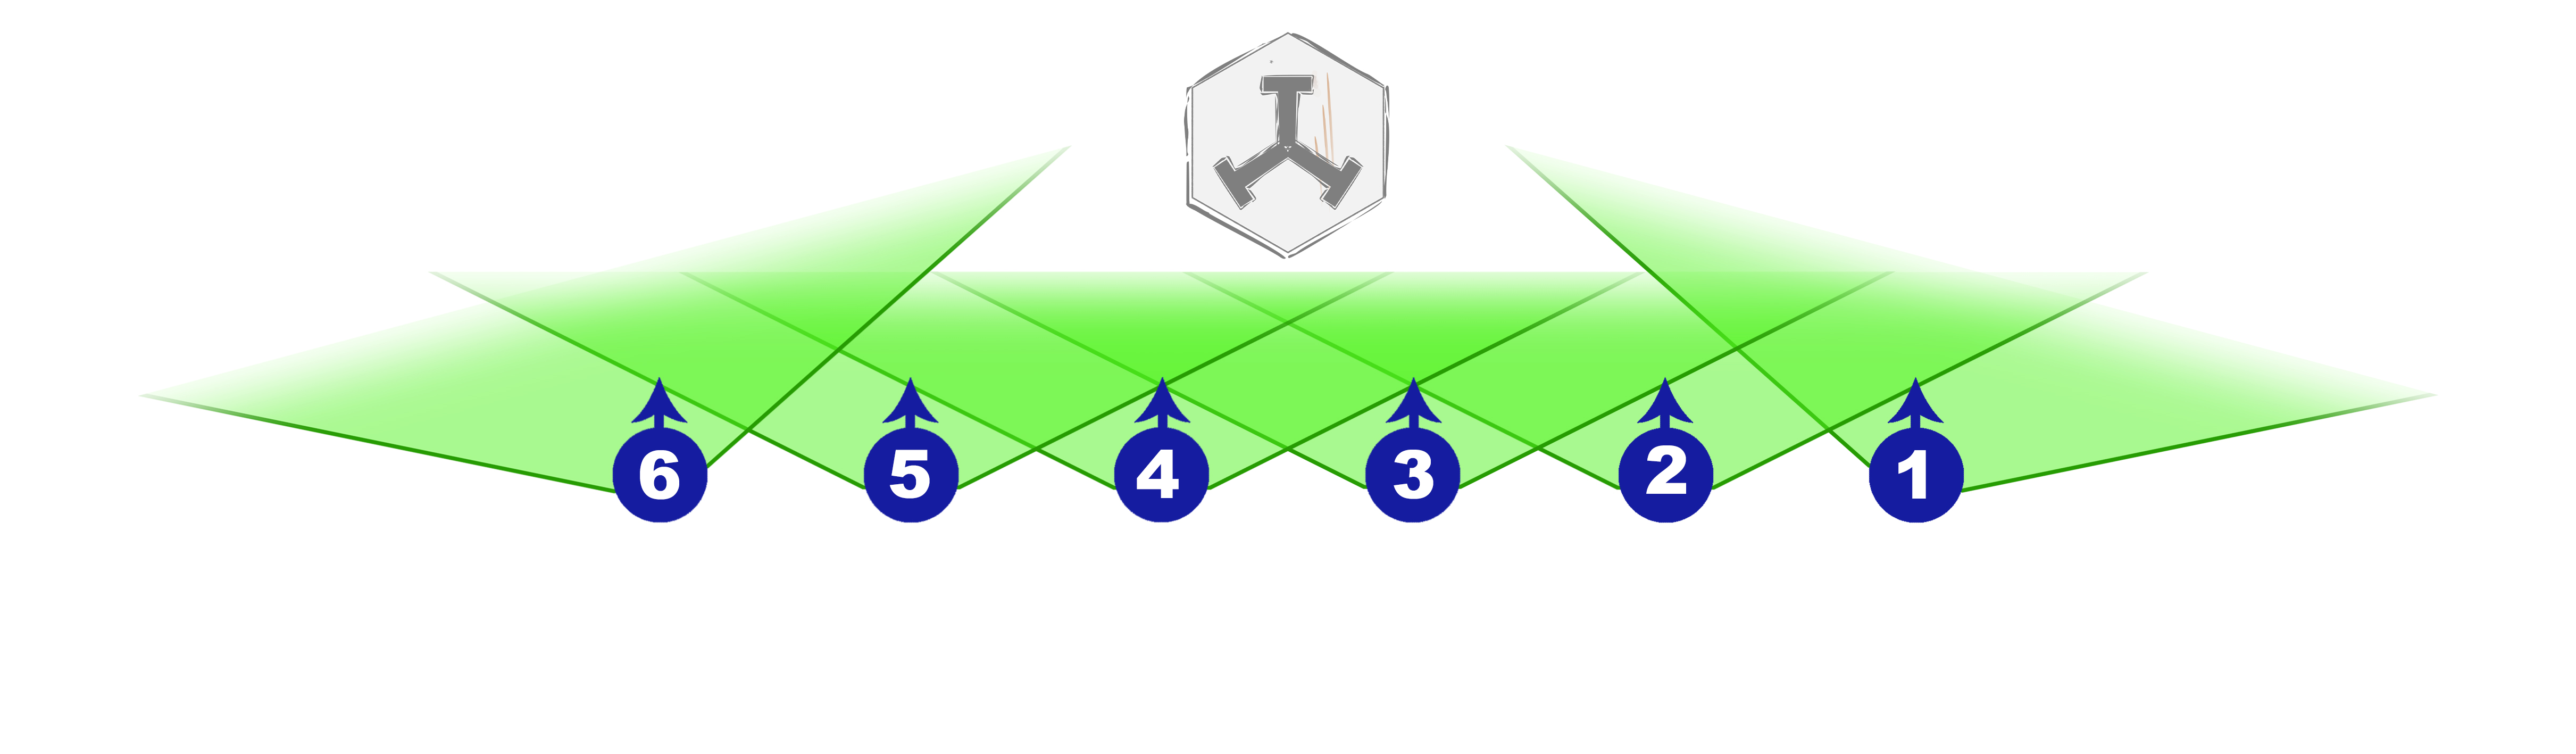
\includegraphics[width=0.95\linewidth]{../img/basic/formation/kette_6mann}
		\caption{Schützenkette}
\end{figure}
\pagebreak

\section{Sicherungsbereiche}
Die Sicherung wird in Bewegung immer über die Uhrzeit ausgegeben. Sowohl in Fahrzeugen als auch zu Fuß in Marschformationen. Die Marschrichtung ist immer 12 Uhr.

\subsection{Rundumsicherung}
Rundumsicherung bedeutet, dass 360° vom Trupp abgesichert werden. Jeder Soldat hat dazu den Auftrag, ein Viertel des \glqq Kreises\grqq\space abzusichern. Eine Rundumsicherung kann aus dem Marsch oder in einer Stellung vollzogen werden. In einer Stellung geht es nicht darum, einen perfekten Kreis zu bilden -- sondern sich in Deckung zu bewegen und von dort aus seinen Sektor zu sichern. Je nach Bedarf kann der Truppführer sich, um z.\,B. zu funken, eine 4 Mann Sicherung aufbauen lassen.
\begin{table}[h]	
	\caption{Sicherungsbereiche der Rundumsicherung für Soldaten}
	\vspace{2.5mm}
	\label{tab:360er}
	\centering
	\begin{tabular}{lll}
		\toprule
		Nr. & Sicherungsrichtung 4 Mann & Sicherungsrichtung 6 Mann\\
		\midrule
		1 & 12 Uhr 	& 12 Uhr\\
		2 & 9 Uhr	& 12 Uhr\\
		3 & 3 Uhr	& 3 Uhr\\
		4 & 6 Uhr	& 6 Uhr\\
		5 &			& 9 Uhr\\
		6 &			& 6 Uhr\\
		\bottomrule
	 \end{tabular}
\end{table}
		
\begin{figure}[h]
	\centering
	\subfigure[4-Mann 360er]{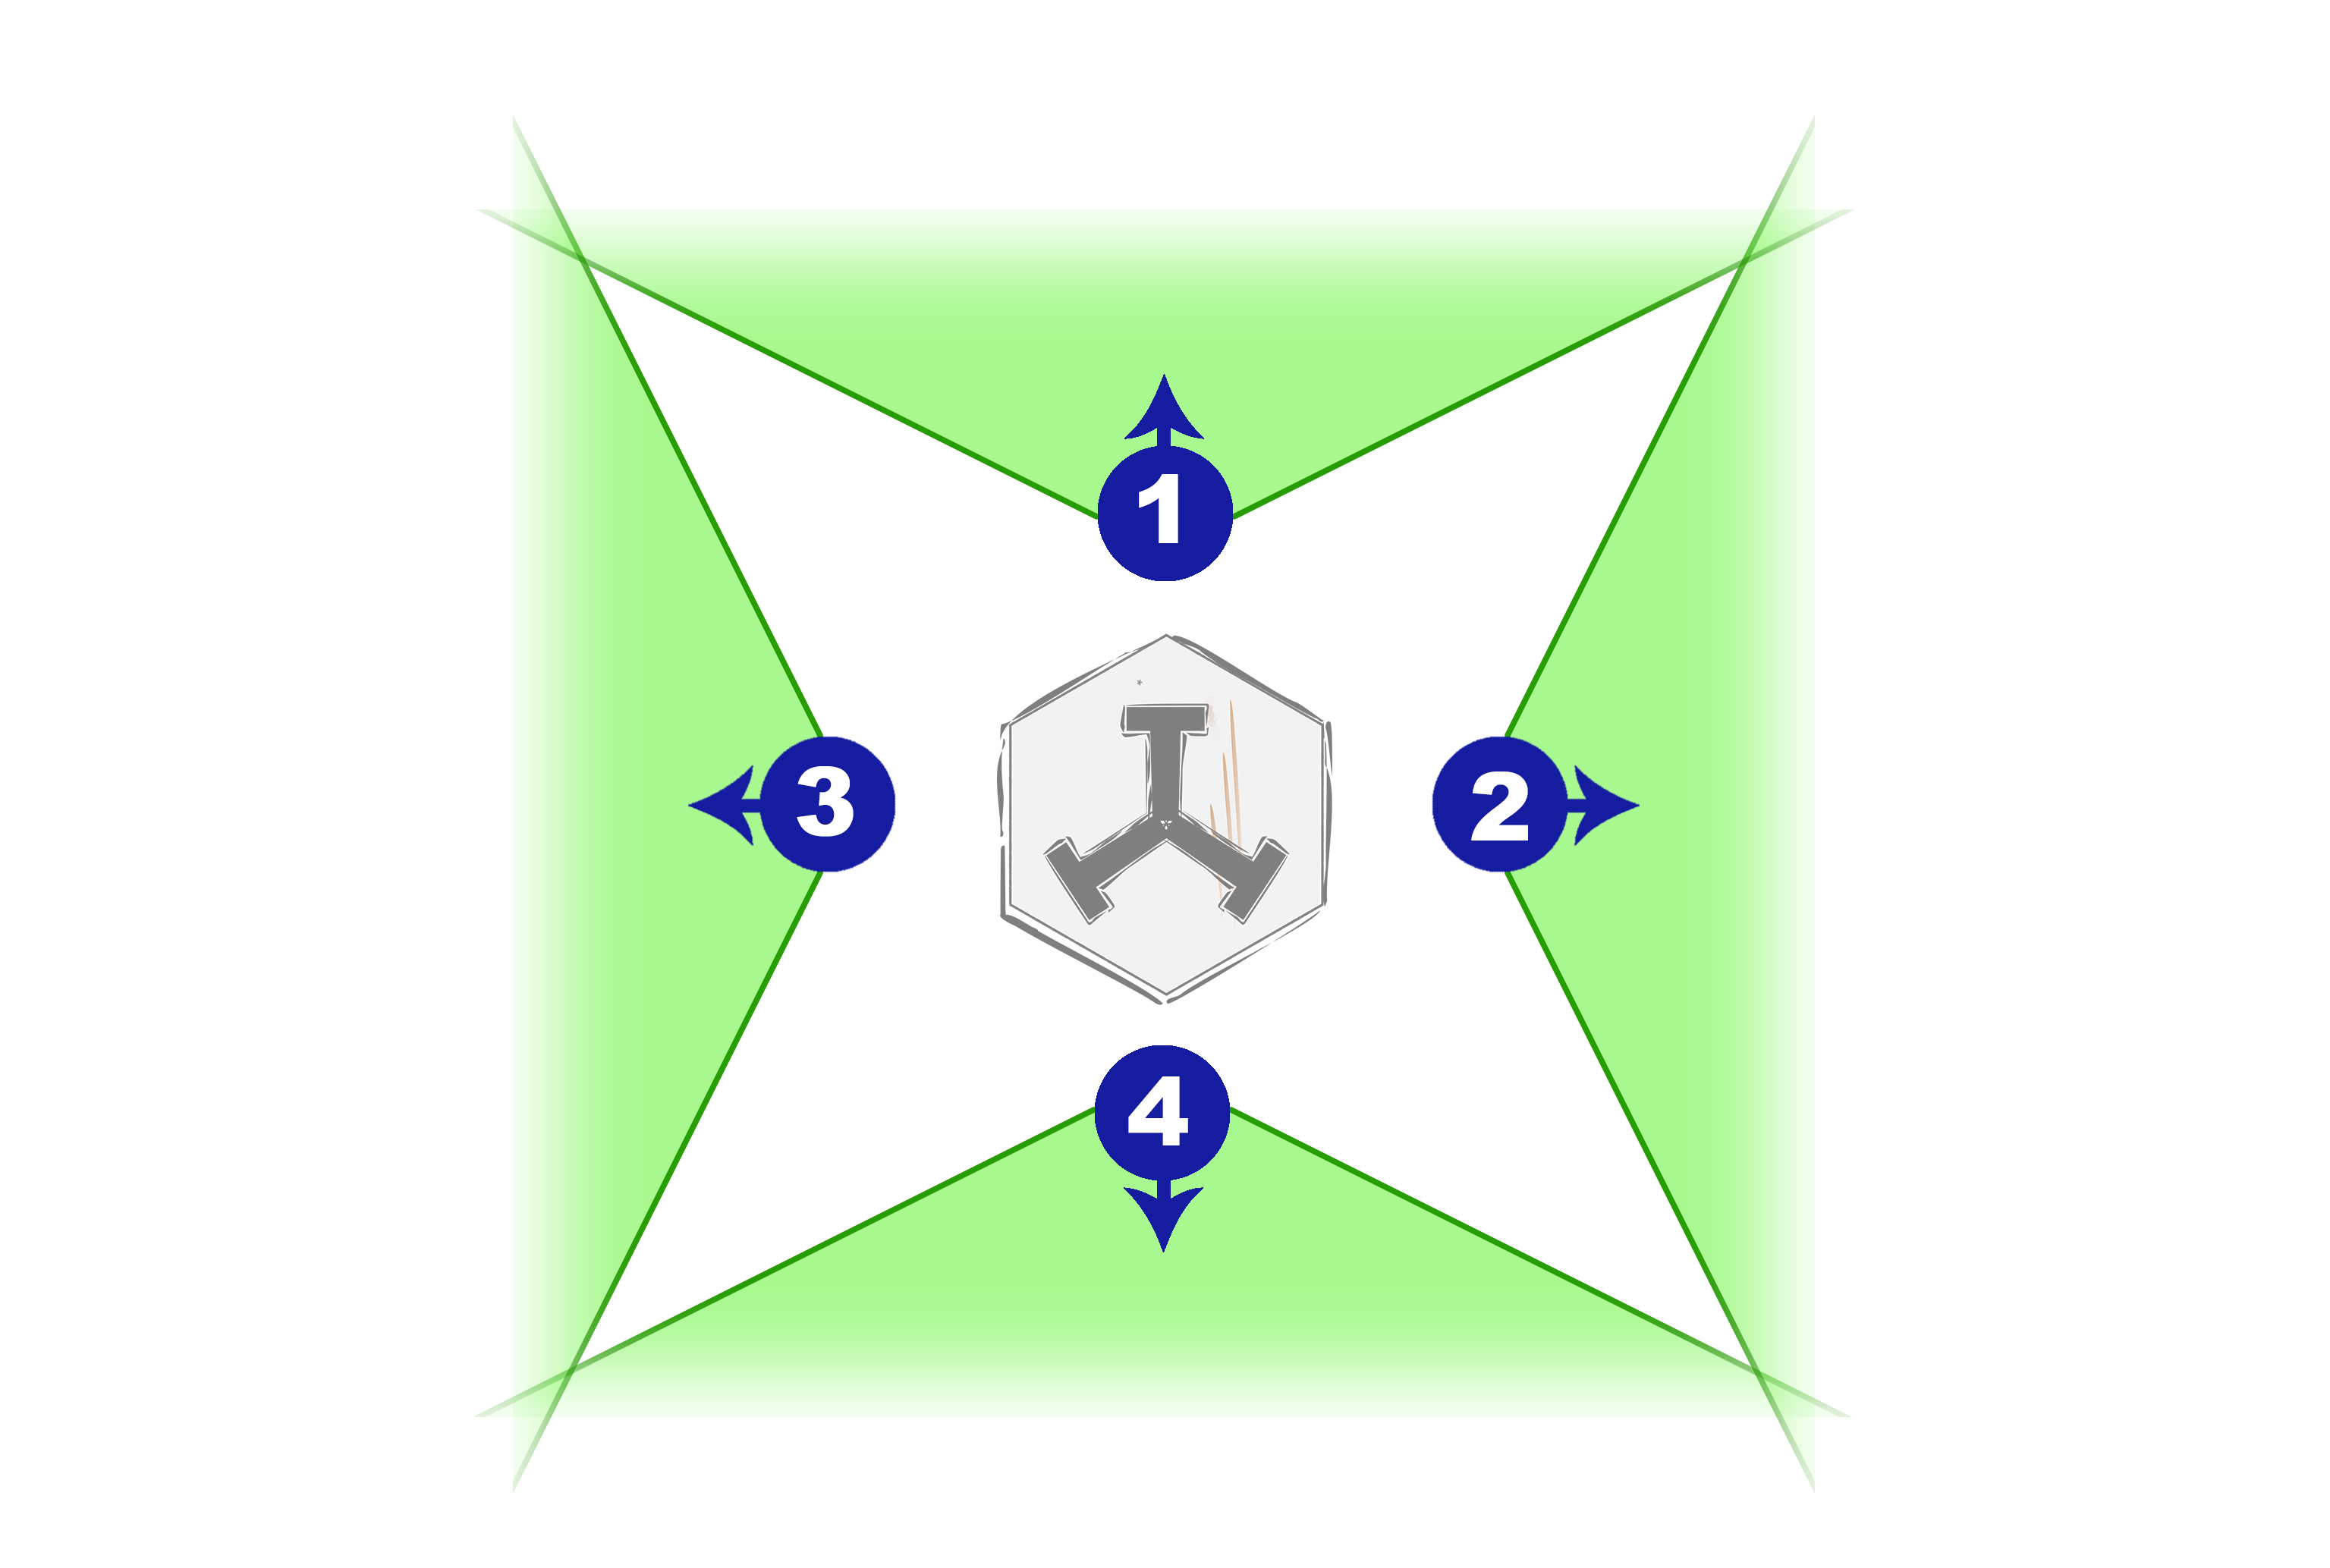
\includegraphics[width=0.49\linewidth]{./img/basic/sicherung/360grad_sicherung_4mann}}
	\subfigure[6-Mann 360er]{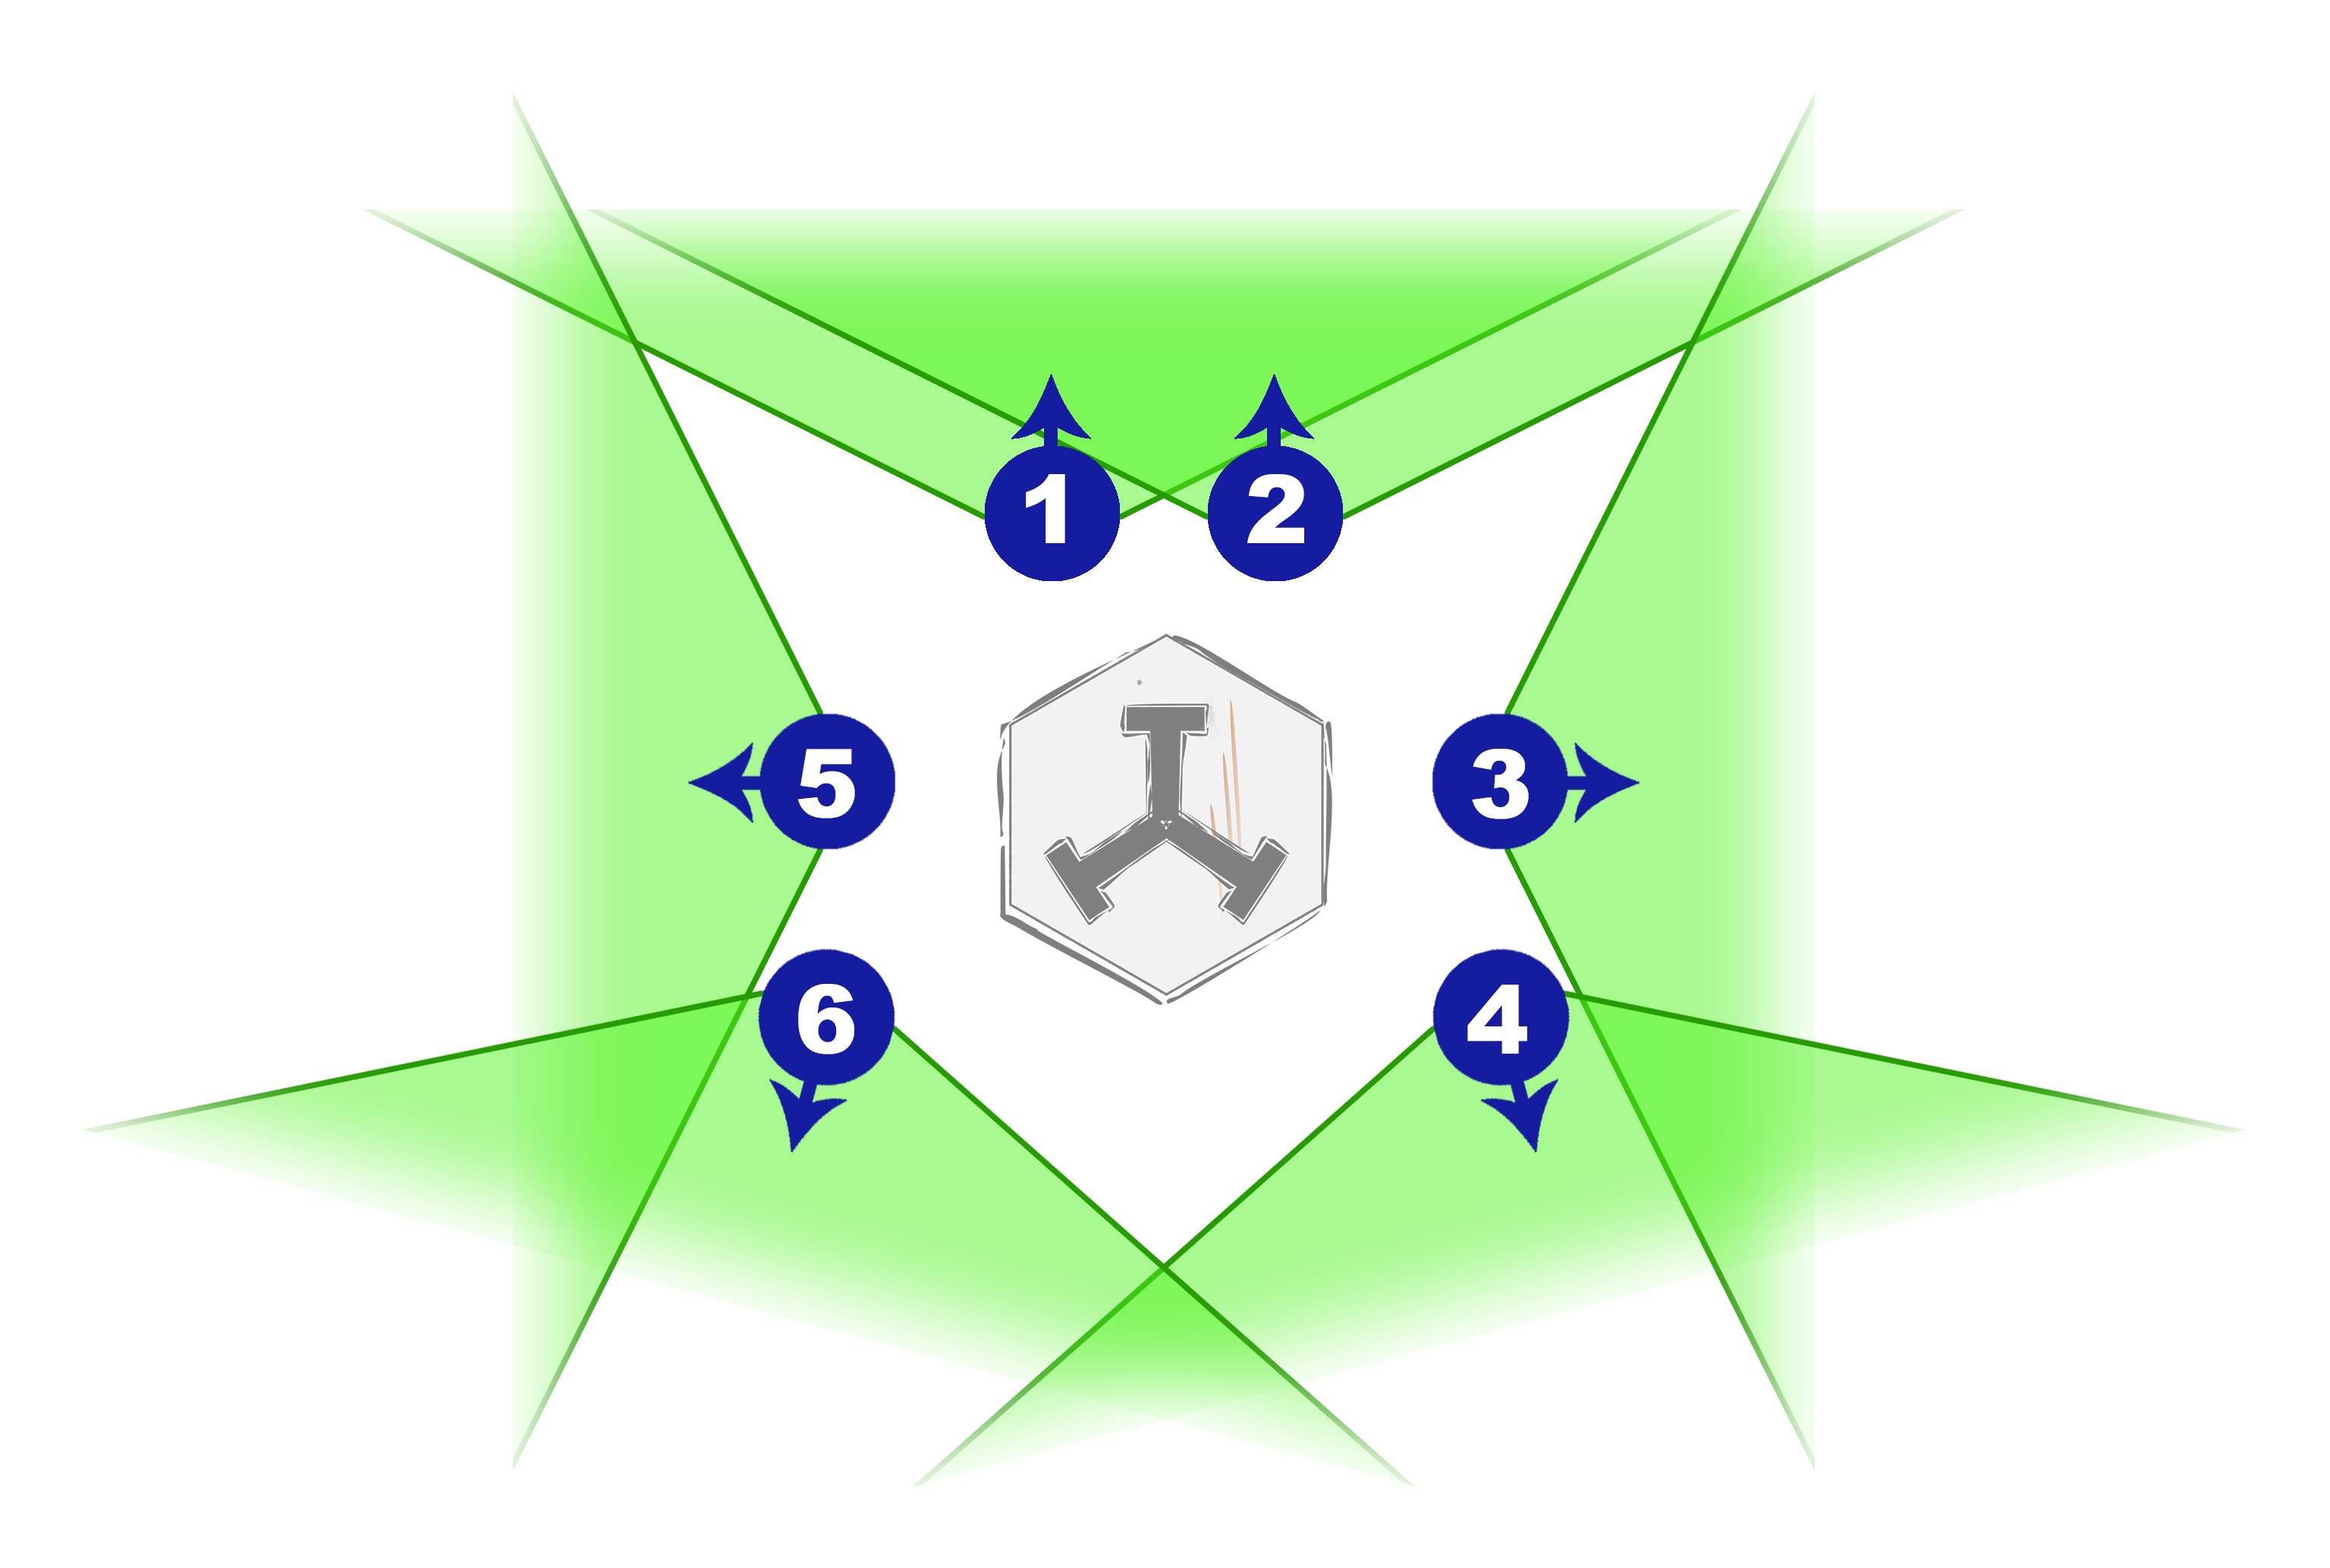
\includegraphics[width=0.49\linewidth]{./img/basic/sicherung/360grad_sicherung_6mann}}
	\label{fig:360er}
\end{figure}

\subsection{180°"=Sicherung}
	Die 180-Grad-Sicherung ist eine Halbkreis-Sicherung. Sie wird in der Regel an Mauern angewandt oder in einer Stellung, um ein zu beobachtendes Gelände abzusichern, wenn der Rückraum als absolut sicher gilt. Zu beachten ist, dass die 180° Sicherung nicht unmittelbar an der Mauer sondern etwa 1m entfernt aufgebaut wird. So können einzelne Soldaten oder Trupps hinter der Sicherung kreuzen, ohne in den eigenen Feuerbereich treten zu müssen.\\
	\begin{figure}[htbp]
		\centering
		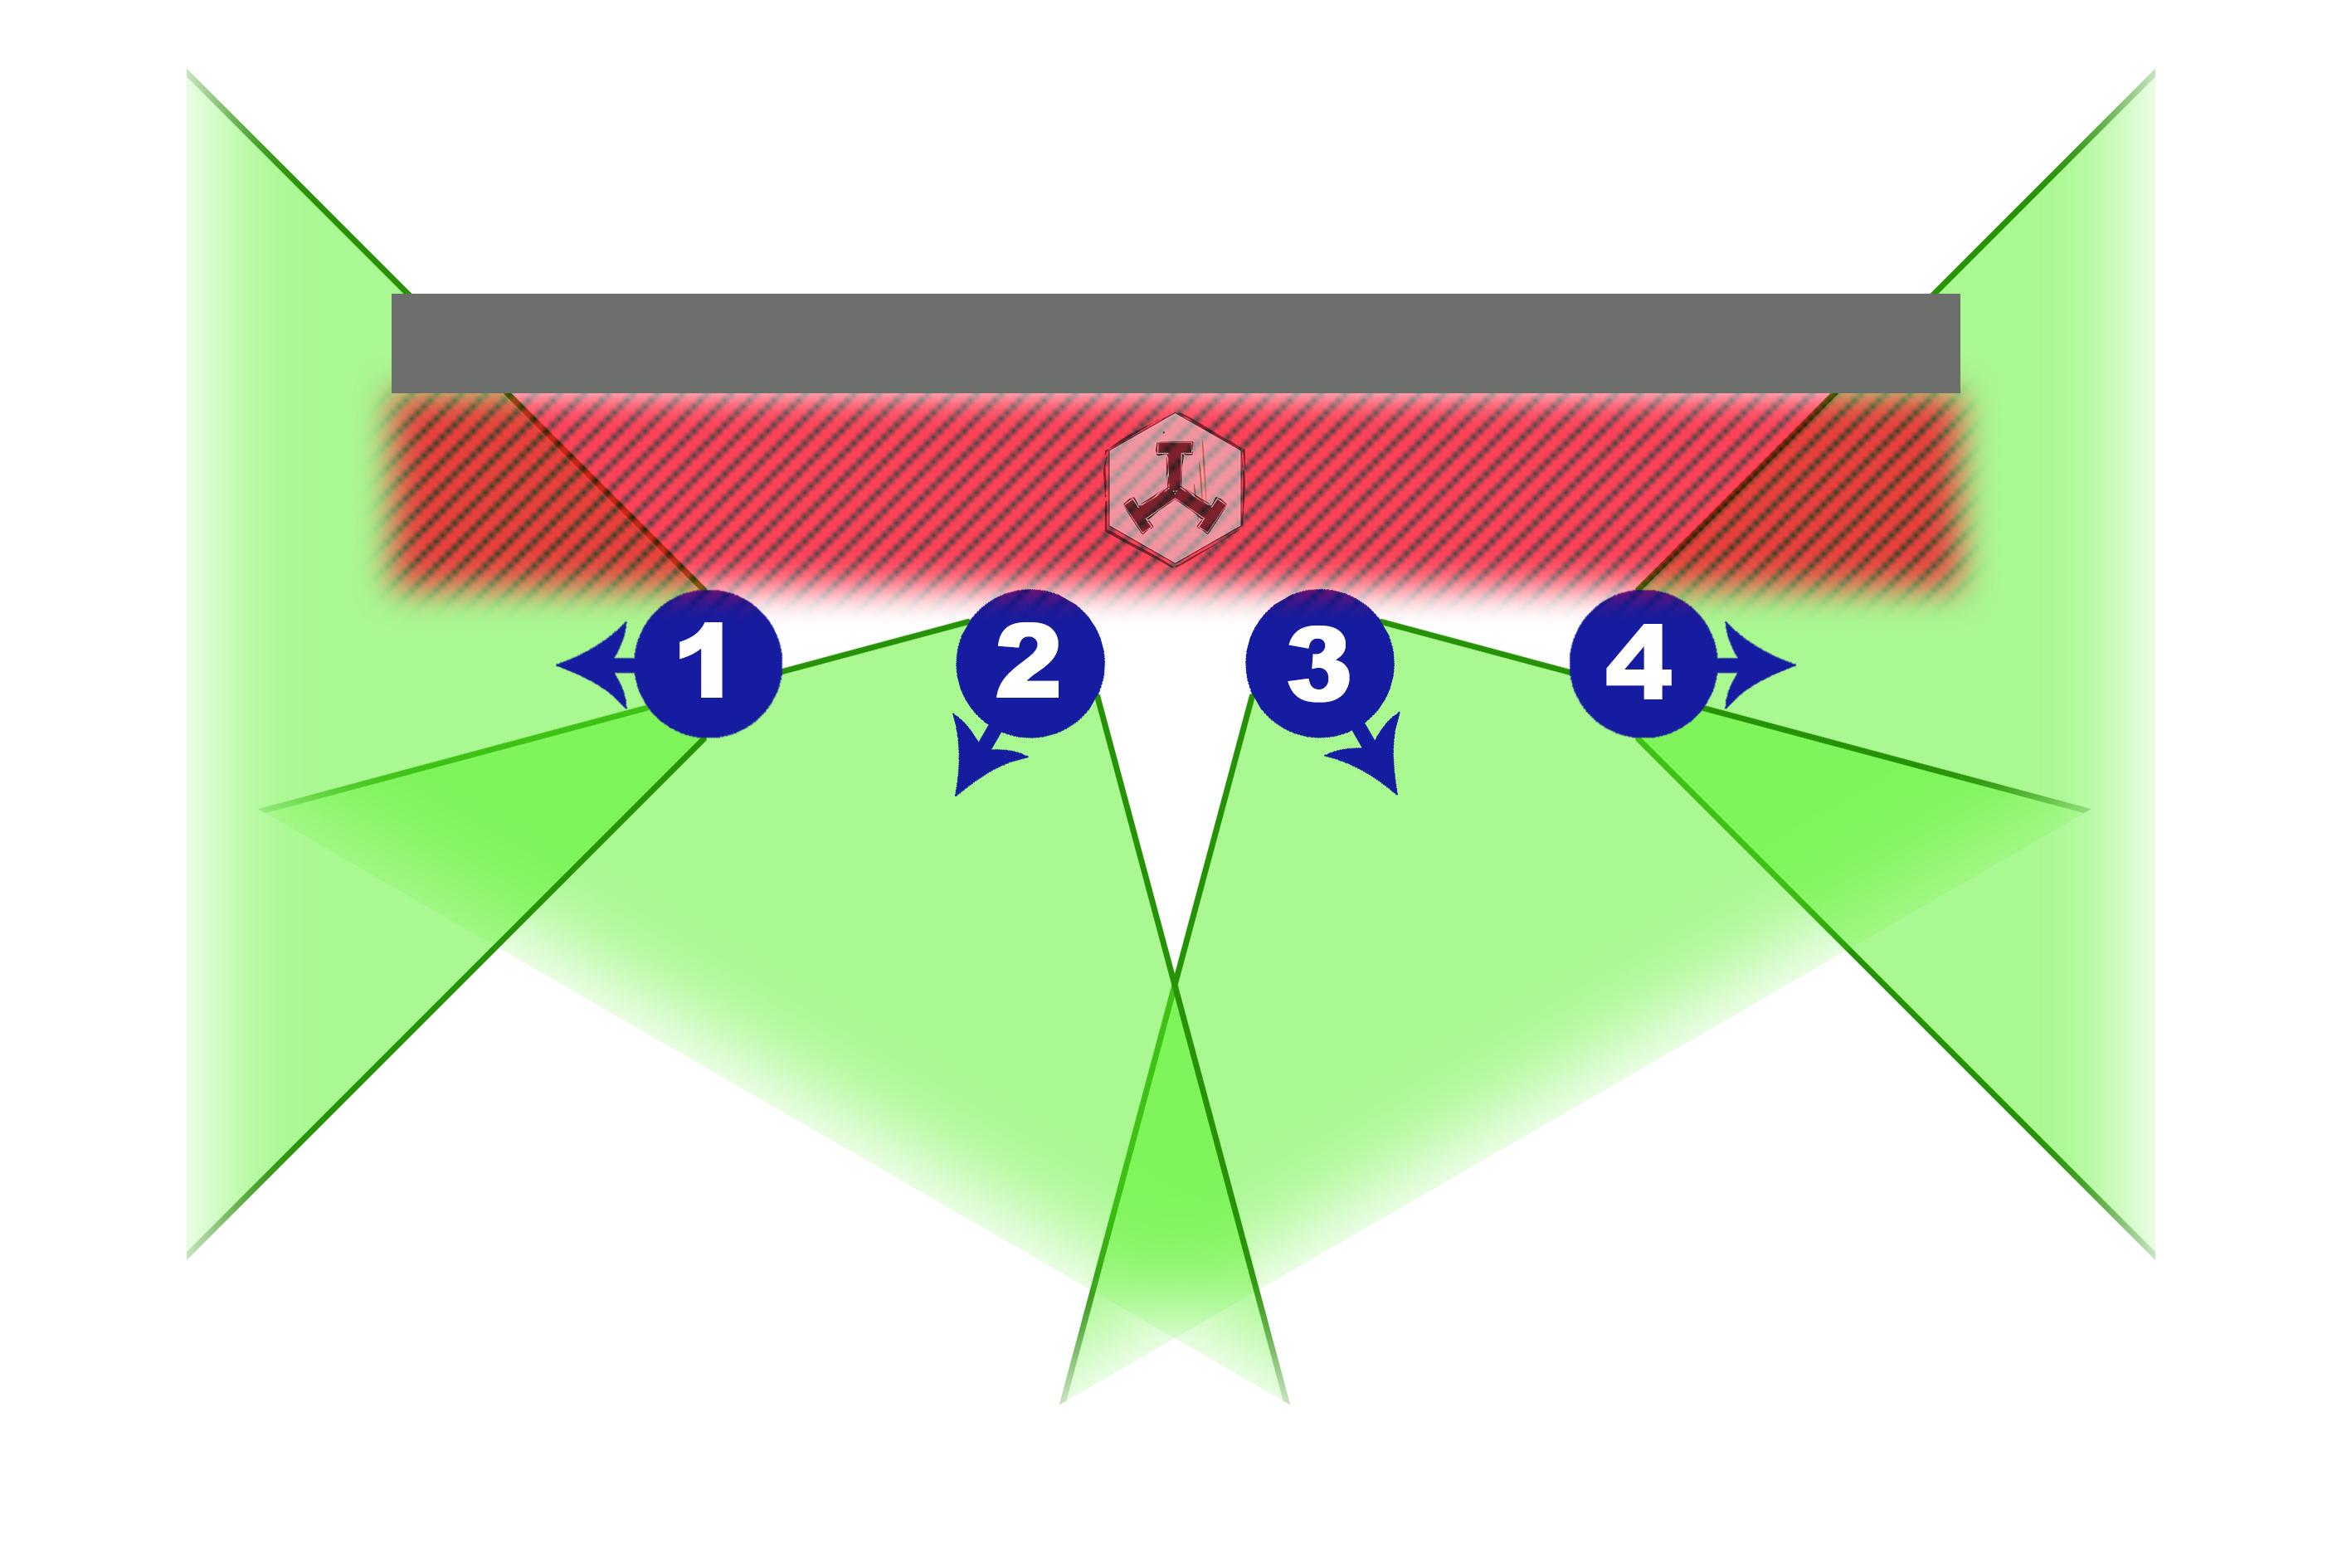
\includegraphics[width=0.8\linewidth]{./img/basic/sicherung/180grad_sicherung_4mann}
		\caption{180° Sicherung an Mauer 4 Mann}
	\end{figure}
		
		\begin{figure}[htbp]
			\centering
			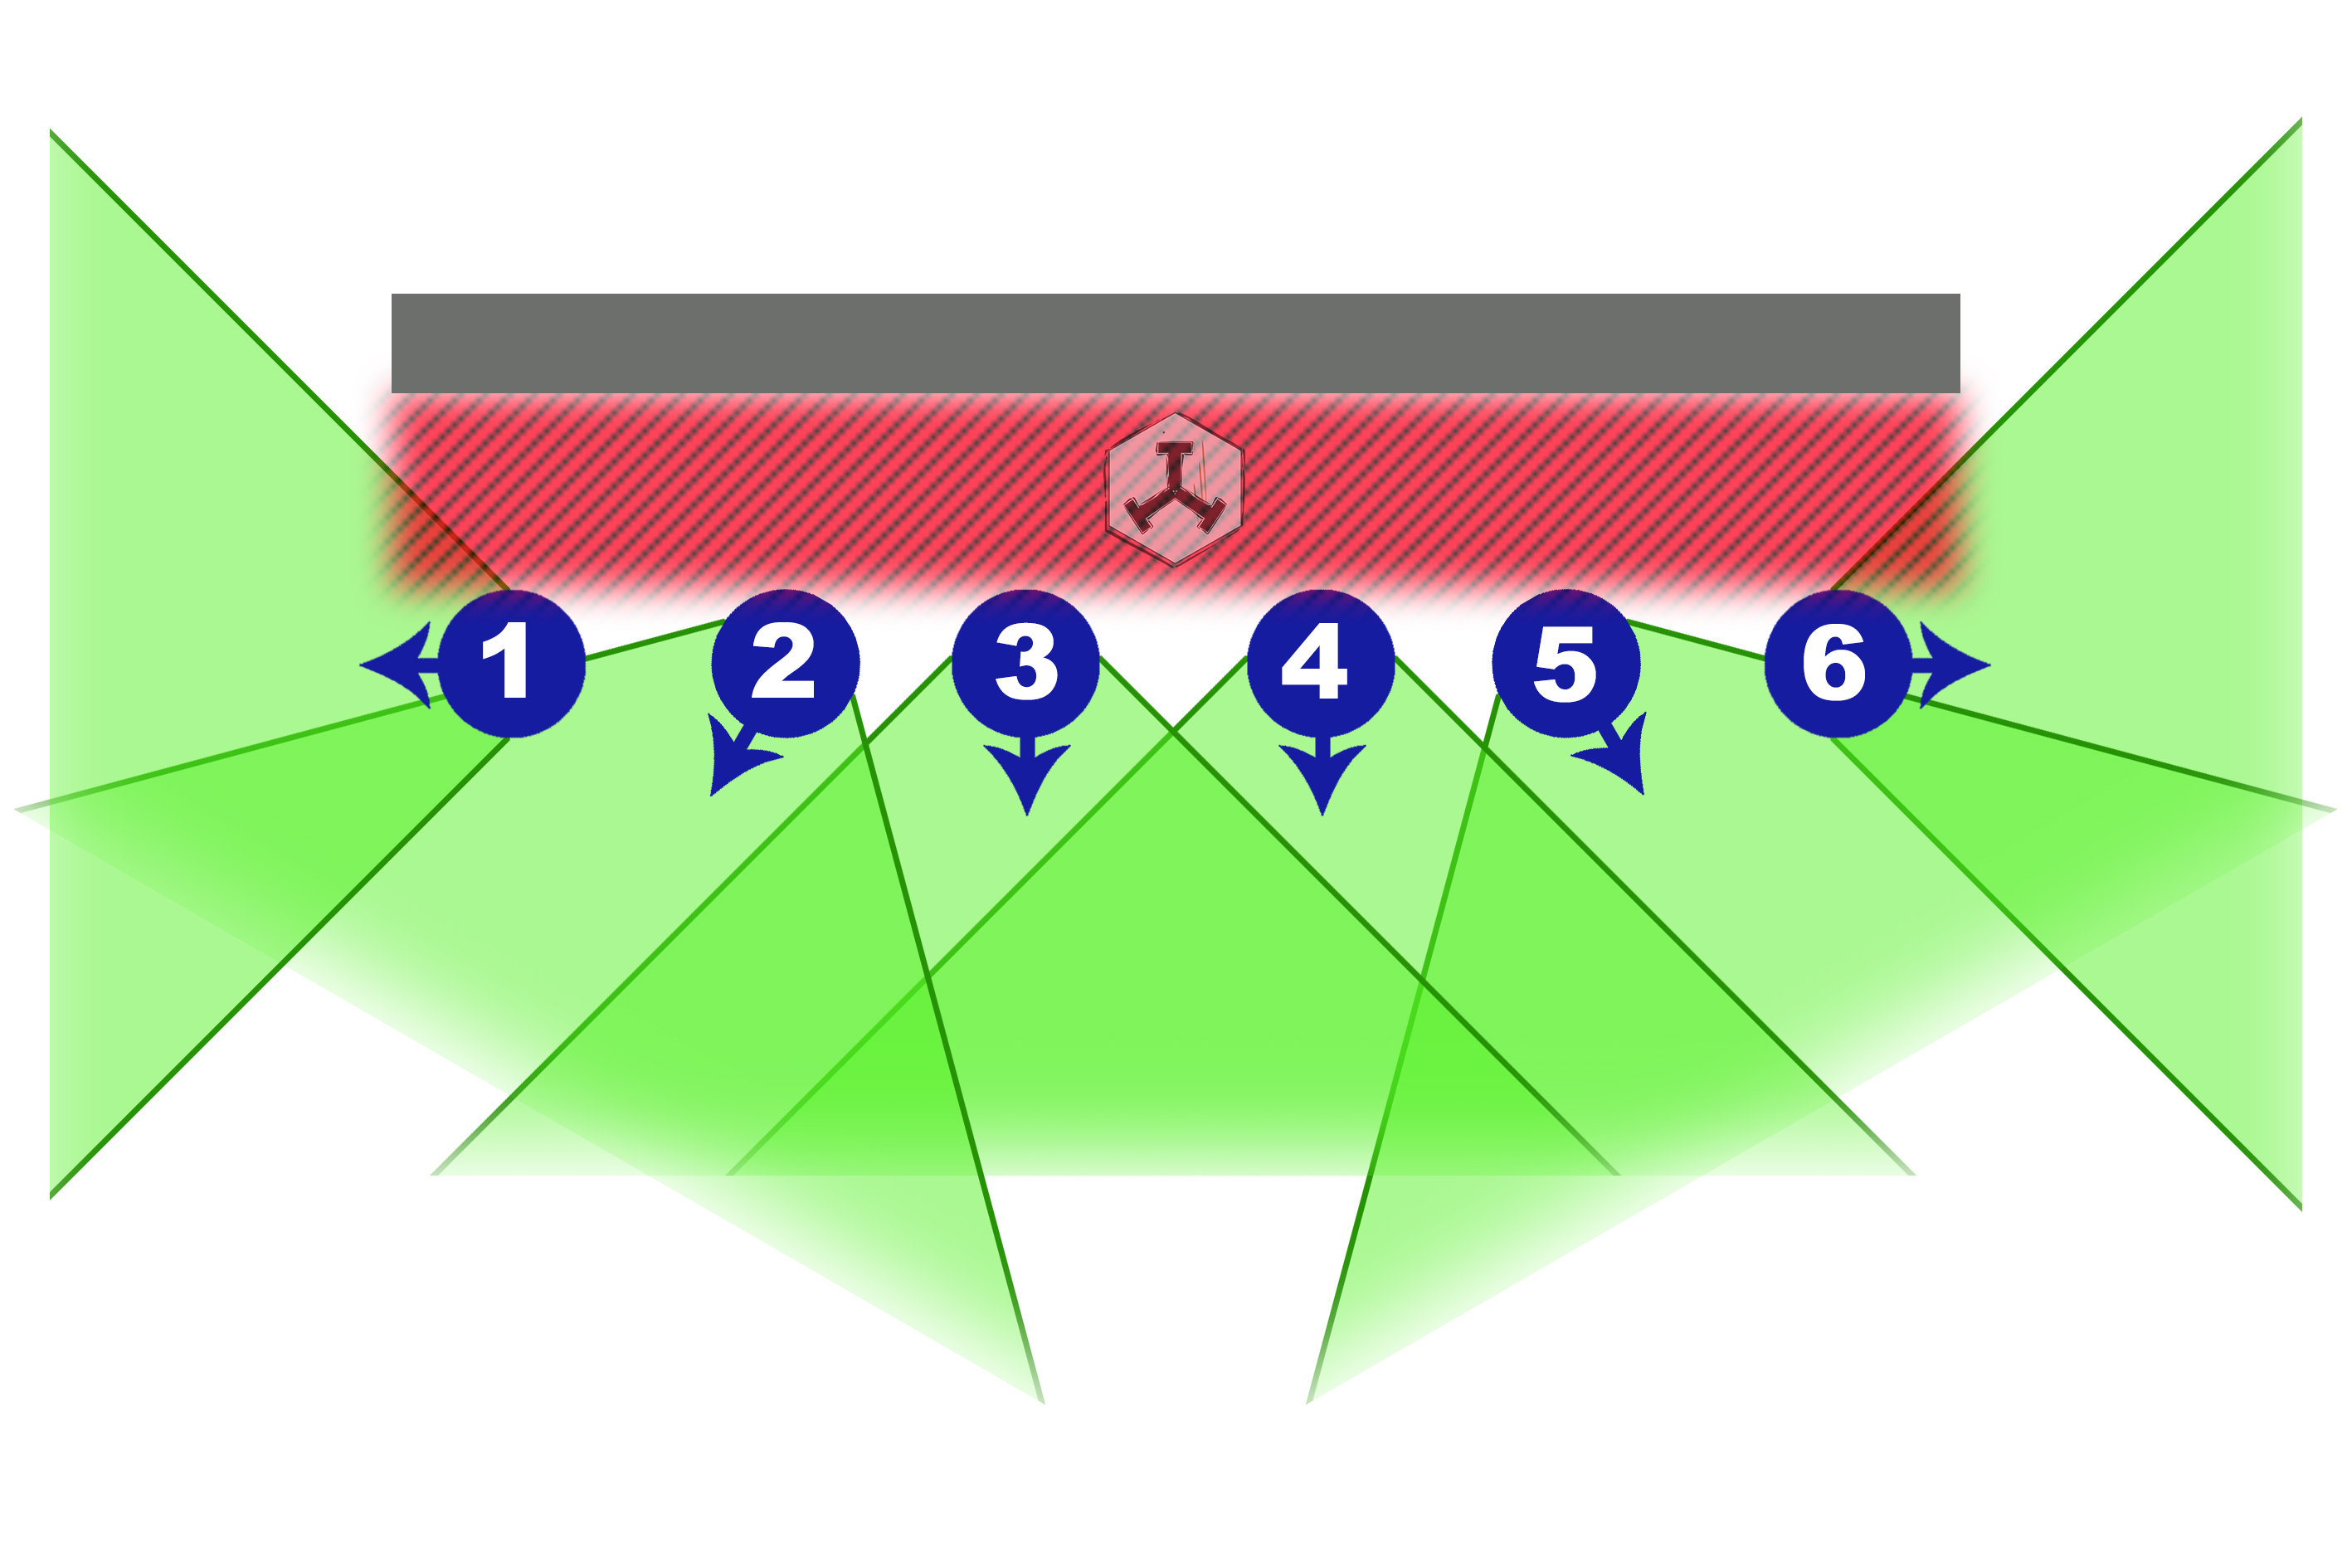
\includegraphics[width=0.8\linewidth]{./img/basic/sicherung/180grad_sicherung_6mann}
			\caption{180° Sicherung an Mauer 6 Mann}
		\end{figure}
\newpage
\section{Das Buddy-System}
	Das Buddy"=System ist ein grundlegender Bestandteil des \textbf{TTT}s (\ref{sec:Grundsaetze}). Dabei ist das Buddy"=Team die kleinste organisatorische Einheit, das solide Fundament jedes Trupps und die Lebensversicherung jedes Soldaten. Damit dieses System funktioniert ist es erforderlich, dass die Buddy"=Mitglieder aufeinander aufpassen, an einem Strang ziehen und sich gegenseitig unterstützen. Weiterhin können Buddy"=Teams als eine Einheit agieren, die spezielle Aufgaben übernehmen. Beispiele hierfür wären Schwerpunktwaffen, Fahrzeugbekämpfung, Aufklärung oder Führung, um nur einige Möglichkeiten zu nennen. Gegenüber den genannten Vorteilen existieren auch Nachteile, die nicht ungenannt bleiben sollen. Ein leicht erkenntlicher Nachteil ist, dass ein Buddy"=System aus Menschen besteht, die zusammenarbeiten müssen. Bis dieses Team optimal zusammenwirkt, kann unterschiedlich viel Zeit vergehen. Dies kann jedoch unter regelmäßiges anwenden beschleunigt werden. Weiterhin können die Spezialisierung von Buddy"=Teams in gewissen Situationen von Nachteil sein. Dies kann jedoch durch den Truppführer kompensiert werden. Damit das Buddy"=System alle Qualitäten hervorbringt sollte jeder Spieler, sowohl Stammspieler, als auch Gast, danach streben ein besserer Buddy zu werden.
	\par\medskip
	Während der Mission sollte sich ein Spieler über folgenden Dinge seines Buddys im Klaren sein:
	\begin{itemize}
		\item Position
		\item Zustand 
		\item Ausrüstung und momentaner Munitionsstand
		\item Grobe Blickrichtung oder Sicherungsrichtung
	\end{itemize}
	Diese Informationen sollten durch die Kommunikation mit seinen Buddy aktuelle gehalten werden (kleine Kampfgespräch). Beispiele hierfür sind z.\,B. die Beobachtungsrichtung, Feindbekämpfung, Positionswechsel oder Richtungsänderungen. Im  \ac{CQB} erfolgt die Kommunikation in anderer Form (siehe CQB). %TODO REF CQB
	Nicht zu vergessen ist, dass Eigensicherung vor Fremdsicherung geht. Das heißt, der Buddy wird erst dann gerettet, wenn sichergestellt ist, dass die Rettung erfolgreich verläuft. Denn ein verletzter Buddy kann seinen Buddy nicht effektiv helfen.
\section{Funken und Kommunikation}
	Zum generellen Gebrauch des Funkgeräts sei auf den TFAR-Mod verwiesen. Weiterhin sollte die eigene Stimmlautstärke nicht auf >>Laut<<, (>>yelling<<) stellen. Dies verhindert, dass die Kommunikation, mehreren eng geführten Trupps, vermischt wird.\\
	Grundsätzlich sollten alle wichtigen Meldungen dem Truppführer, über die Trupp interne Funkfrequenz, mitgeteilt werden.
 
\subsection{Kontakmeldungen}
	Kontaktmeldungen sollten im Optimalfall nach einem bestimmten Schema ablaufen. Hierbei gilt im Gefecht wird nicht jede Kontaktmeldung perfekt sein. Dennoch sollte die Meldung möglichst nach diesen Schema erfolgen.
	\begin{itemize}
		\setlength{\itemsep}{-4pt}
		\itemsep-4pt
		\item >>Kontakt<< oder >>Freunde<<
		\item Anzahl 
		\item Was
		\item Wo (Grobe Richtung, Landmarke (ggf. verfeinern), Gradzahl auf Kompass) 
		\item Entfernung
		\item Weitere Angaben (Bewaffnung, Alarmzustand (heiß oder kalt), Bewegungsrichtung, ...)
	\end{itemize}

	Beispiele:
	\begin{longtable}{P{0.95\linewidth}}
	\toprule
	Kontakt -- 1 feindlicher \acs{SPZ} -- auf 4 Uhr -- Rechts über der Hütte -- auf 95° -- ca. 500m\\
	\rcg Kontakt -- 3 Infanteristen -- auf 1 Uhr -- Kommen über den Hügel -- bei 25° -- ein \acs{MG} -- ca. 300m -- kalt\\
	\bottomrule
	\end{longtable}	
\subsection{Funkgespräch unterbrechen}
	In bestimmten Situationen ist es erforderlich eine aktuelle Funkmeldung oder ein Gespräch zu unterbrechen, um eine Meldung abzusetzen von höherer Priorität, wie z.\,B. Feindkontakt zu melden. Dabei stellt >>Break, Break<< eine kurze und prägnante Aussage dar.\\
	Beispiel:
	\begin{longtable}{P{0.95\linewidth}}
	\toprule
	TF: >>Wir gehen folgendermaßen vor Bud\dots<<\\
	\rcg TM: >>Break, Break<< \dots >>Kontakt feindlicher Trupp auf 2 Uhr 100\,m nähert sich<<\\
	TF: >>Verstanden, Feuer frei!<<\\
	\bottomrule
	\end{longtable}		

\subsection{Sonstige Meldungen}
	\paragraph*{Betreten von Fahrzeugen}
	\label{para:fahrzeug-betreten}
	Bei betreten oder verlassen von Fahrzeugen wird kurz und prägnant gemeldet, dass der Soldat das entsprechend Betreten betreten oder verlassen hat. Damit erhält der TF die Information wo sein Trupp sich befindet und die Truppmitglieder wissen wie sie sich zu verhalten haben. (Erst wenn 3 meldet, dass er sitzt kann 2 aufsitzen)\\
	Beispiel: >>3, Sitzt<<

	\paragraph*{Sicherungsposition melden}
	Meldungen über aufgebaute Sicherung sind nützlich Details, die den TF über den Status der Sicherung informieren. \\
	Beispiel: >>Hier 6, Sicherung nach 6 Uhr steht<<

	\paragraph*{Trupp in Bewegung}
	Das letzte Truppmitglied (üblw. die Nr.\,6) meldet den Status der Bewegung.\par
	Beispiel:
	\begin{longtable}{P{0.95\linewidth}}
	\toprule
	TF: >>Trupp Marsch<<\\
	\rcg TM 6: >>Trupp in Bewegung<<\\
	\bottomrule
	\end{longtable}		
	
	\paragraph*{Statusmeldung und durchzählen}
	\label{sec:Status}
	Nach heftigen, ggf. unübersichtlichen Feindbeschuss ist es sinnvoll den Status des Trupps abzufragen. Die Meldung gibt den Gesundheitsstatus und Munitionsstatus, mittels Ampelsystem durch. Sollte der Truppführer nicht erreichbar sein kann auch ein Trupp Mitglied die Statusabfrage anordnen.\par
	Es wird generell von 1 an heruntergezählt. (Wenn 1 die Statusmeldung anordnet entfällt die Meldung der 1 i.\,d.\,R.)  \\
	Aufbau der Meldung: >>Nummer, Gesundheitsstatus, ggf. Besonderheiten<<
	\par\medskip
	Beispiel:
	\begin{longtable}{P{0.95\linewidth}}
	\toprule
	>>1 hier 5, Kommen<< \dots (keine Reaktion)\\  
	>>Hier 5, Trupp Status durchgeben<< \dots (kurz warten 1 und 2 melden sich nicht)\\ 
	\rcg >>Hier 3, Status Rot, Gelb<< \dots\\ 
	\rcgg >>Hier 4, Status Grün, Grün, zwei Verletzte auf dem Hügel<< \dots usw.\\
	\bottomrule
	\end{longtable}		

\subsection{Wichtigste Funkabkürzungen und Begriffe}
	\begin{longtable}{p{0.1\linewidth}p{0.25\linewidth}p{0.05\linewidth}p{0.1\linewidth}p{0.35\linewidth}} 
		\toprule
		\acs{SPZ}	& \acl{SPZ}	&& Standby	& Bitte warten \hfil\\ 
		\midrule
		\acs{KPZ}	& \acl{KPZ}	&& Kalt		& keine Gegner; Gegner haben uns nicht erkannt\\ 
		\acs{AA}	& \acl{AA}	&& Heiß 		& Gegner eröffnen Feuer, haben uns entdeckt \\ 
		\acs{AT}	& \acl{AT}	&& \acs{OPL}	& \acl{OPL} \\ 
		\acs{MG}	& \acl{MG}	&& \acs{CAS}	& \acl{CAS} \\ 
		\bottomrule
	\end{longtable}




  
\subsubsection{Kommandos -- die wichtigsten Befehle}
\label{sec:kommando}
\paragraph*{Kommando: >>Deckung!<<}\hfil\\
	Die Deckung ist ein situationsbedingter Aufenthaltsort.\\ 
	Wird man vom Feind überrascht, ist der Soldat angewiesen, sofort Deckung im nahen Umfeld (Radius 20 Meter) zu suchen – ohne die Trupp-Struktur aufzulösen. Dabei gilt zu beachten, dass die Buddy-Teams immer im Verbund bleiben. \\
	Als Deckung zählt alles, was als beschusssicher gilt: Häuser, Felsen, Mauern, Senken. Ist keine Deckung in Laufweite, wird sofort Bodenlage eingenommen und auf den Feind ausgerichtet. Bei indirektem Beschuss (Granaten, etc.) wird ein besonders weiter Abstand zwischen den Kameraden gesucht.\\

	Der Befehl vom Truppführer lautet >>Deckung!<< oder als ausführlicheres Beispiel >>Deckung, 6 Uhr, hinter der Mauer!<<

\paragraph*{Kommando: <<Bezieht Stellung bei \dots!>>}\ \\
	Die Stellung ist ein selbst gewählter Aufenthaltsort. \\
	Die Stellung ist idealerweise ein gewählter und geschützter Aufenthaltsort (Haus, Senke, Felsen, Mauer) und lässt sich leicht verteidigen. Die Soldaten haben dabei maximale Deckung eingenommen und sichern. \\
	Der Truppführer gibt den Befehl aus, um einen Aufenthaltsort festzulegen, wo sich der Trupp aufhalten soll. Daraus folgt automatisch, dass der Trupp den Ort erreicht und vorläufig sichert. Der Sicherungsschwerpunkt liegt automatisch auf vermutete Feindstellungen. Mit dem Zusatz <<gedeckt>> betont er, dass der Trupp eine Aufklärung durch den Feind unter allen Umständen vermeiden soll. In der Praxis: Nähern in die gedeckte Stellung unter Sicht- und Deckungsschutz. Dort in die Stellung getarnt beziehen und halten. In der Stellung erfolgt vom Truppführer:

\paragraph*{Kommando: >>Bekämpfen  \dots!<<}\hfil\\
	Der Soldat soll einen erkannten Feind bekämpfen. Hierbei ist es wichtig, genau abzuwägen, wie viel Einweisung benötigt wird, damit das Kommando erfolgreich ausgeführt werden kann. Der Soldat meldet bei erfolgreicher Absolvierung des Auftrags >>Gegner, YXZ, bekämpft!<<

\paragraph*{Kommando: >>Feuer frei!<<}\hfil\\
	Das ist die direkte Anweisung, JETZT zu schießen. Kann ergänzt werden mit >>Feuern, 3 Salven<< oder sonstigen Einschränkungen.

\paragraph*{Kommando: >>Unterdrückungsfeuer!<<}\ \\
	Das ist die direkte Anweisung, in die generelle Richtung des Gegners zu schießen, um ihn in die Deckung zu zwingen und ihn an Gegenfeuer oder Manövern zu hindern.

\paragraph*{Kommando >>Gezieltes Feuer!<<}\hfil\\
	Das ist die direkte Anweisung, den Gegner mit gezielten Salven oder Einzelschüssen direkt zu treffen -- also das Gegenteil vom Unterdrückungsfeuer. In der Regel wird bei der Feuerfreigabe erwartet, dass gezieltes Feuer abgegeben wird.

\paragraph*{Kommando >>Feuerfreigabe erteilt<<}\hfil\\
	Grundsätzliche Freigabe den Feuerkampf eigenständig zu eröffnen. Das heißt, sobald Gegner in Sicht sind und der Feuerkampf ist aussichtsreich, darf geschossen werden. Dies gilt bis zum Widerruf.

\paragraph*{Kommando >>Feuer nur auf Freigabe<<}\hfil\\
	Vor dem Schuss muss Feuerfreigabe angefordert werden.

\paragraph*{Kommando: >>Stopfen!<<}\hfil\\
	Der Soldat stellt sofort das >>Schießen<< ein.

\paragraph*{Kommando: >>Bezieht Stellung bei \dots!<<}\hfil\\
	Die Stellung ist ein selbst gewählter Aufenthaltsort. Idealerweise ist diese ein geschützter Aufenthaltsort (Haus, Senke, Felsen, Mauer) und lässt sich leicht verteidigen. Die Soldaten haben dabei maximale Deckung eingenommen und sichern.\\
	Der Truppführer gibt den Befehl aus, um einen Aufenthaltsort festzulegen, wo sich der Trupp aufhalten soll. Daraus folgt automatisch, dass der Trupp den Ort erreicht und vorläufig sichert. Der Sicherungsschwerpunkt liegt automatisch auf vermutete Feindstellungen. Mit dem Zusatz >>gedeckt<< betont er, dass der Trupp eine Aufklärung durch den Feind unter allen Umständen vermeiden soll. In der Praxis: Nähern in die gedeckte Stellung unter Sicht- und Deckungsschutz. Dort in die Stellung getarnt beziehen und halten. In der Stellung erfolgt vom Truppführer:
		\begin{itemize}
			\item Kontaktaufnahme mit dem Zugführer 
			\item Geländetaufe 
			\item Verteilung von Feuerbereichen 
			\item Vorausschauende Planung (Wegplanung, Korridore, weitere Stellungen) 
			\item Kommando: <<Bezieht gedeckte Stellung bei \dots!>> 
		\end{itemize}

\paragraph*{Kommando: >>Wechselt die Stellung!<<}\hfil\\
	Der taktische Stellungswechsel ist ein eigenständiger Positionswechsel in eine andere Stellung – beispielsweise, weil man befürchtet, die Stellung ist vom Feind bereits aufgeklärt wurde und damit Feindfeuer erwartet. Das gilt besonders nach Feuerüberfällen – häufige Stellungswechsel sind sehr effektiv um Gegner zu verwirren.

\paragraph*{Kommando: >>Nehmt ein!<<}\hfil\\
	Das bedeutet für den Trupp, dass eine gegnerische Stellung und\,/\,oder ein Gebiet (umkämpft oder nicht umkämpft) unter allen Umständen eingenommen und erobert werden soll. Einnehmen signalisiert dem Soldaten, dass Feindkontakt möglich ist.

\paragraph*{Kommando: >>Haltet \dots!<<}\hfil\\
	Das bedeutet nichts anderes als IN der Stellung zu verbleiben und diese zu verteidigen.

\paragraph*{Kommando: >>Melden bei Vollzug!<<}\hfil\\
	Der Soldat soll, sobald er seinen Auftrag erledigt hat, sich beim Auftraggeber melden. Dies kann per Funk oder direkter Ansprache erfolgen.

\paragraph*{Kommando: >>Status<<}\hfil\\
	Der Soldat gibt den Gesundheitsstatus und seinen Munitionsstatus durch. Dieses Kommando deckt sich mit den Abschnitt \ref{sec:Status}.

\subsubsection{Feuerfreigaben}
	Es versteht sich von selbst, dass wir nicht auf alles zur jeder Zeit schießen können. Daher gibt es die sogenannten Feuerfreigaben, wann geschossen werden darf und wann nicht. Wir unterschieden 3 Typen:

\paragraph*{>>Feuerstatus rot<<}
	Alternativ: >>Status -- Feuer halten<<\hfil\\
	Nur schießen, wenn es um das blanke Überleben geht. >>Feuer halten<< wird ausgegeben, wenn wir leise und unerkannt in eine Stellung einsickern wollen. Feuergefechte sollten unter allen Umständen vermieden werden, da Schüsse die eigene Position verraten und Kameraden gefährden können.

\paragraph*{>>Feuerstatus gelb<<}
	Alternativ: >>Status -- Feuer erwidern<<\hfil\\
	Bei erkanntem Feind, der uns noch nicht uns bekämpft (kalt), wird der Feind gemeldet und es wird gewartet, was der Truppführer entscheidet. Es darf bei Beschuss auf die eigene Stellung zurückgeschossen werden, wenn der Feind klar erkannt wurde (heiß).

\paragraph*{>>Feuerstatus grün<<}
	Alternativ: >>Status -- Feuer frei<<\hfil\\
	Jeder erkannte Feind darf bekämpft werden. Diese Freigabe wird beispielsweise bei einem Feuerüberfall gegeben, oder in einem Verteidigungsszenario aus einer befestigten Stellung heraus.

\subsubsection{Zusammenfassung Kommandos}
	\begin{longtable}{p{0.3\linewidth}p{0.65\linewidth}} 
		\toprule
		\textbf{Befehl} & \textbf{Bedeutung}\\
		\midrule
		Deckung! & Beschusssichere Stellung in 20\,m Umkreis suchen mit Buddy, ansonsten auf den Boden legen.\\
		Bekämpfen! & Erkannten Feind bekämpfen, bei Vollzug mit >>Bekämpft<<, bestätigen.\\
		Feuer Frei! & Feuer sofort eröffnen.\\
		Unterdrückungsfeuer! & Durch gezielte Schüsse in Feindrichtung diesen am kämpfen oder bewegen hindern.\\
		Gezieltes Feuer! & Gegner mit gezielten Salven oder Einzelschüssen bekämpfen. Wird bei \glqq Feuer frei\grqq\, vorausgesetzt.\\
		Feuerfreigabe erteilt! & Ist Feuerkampf aussichtsreich, darf dieser begonnen werden.\\
		Feuer nur auf Freigabe! & Feuerkampf ist nur auf expliziten Befehl hin zu beginnen.\\
		Stopfen! & Das Feuern ist \textbf{sofort} einzustellen.\\
		Bezieht Stellung bei \dots! & Mit Trupp oder Buddy zu einer Position gehen und entsprechende Sicherung aufbauen.\\
		Wechselt die Stellung! & Mit Trupp oder Buddy oder alleine in andere Stellung verlegen.\\
		Nehmt \dots ein! & Das angegebene Ziel ist unter allen Umständen zu erobern und zu sichern.\\
		Haltet! & In der Stellung bleiben und diese verteidigen.\\
		Melden bei Vollzug! & Rückmeldung bei Abschluss eines Befehls oder Auftrags.\\
		Status! & Gesundheitsstatus und Munitionsstatus mit Ampelsystem durchgeben.\\
		\bottomrule
	\end{longtable}

\pagebreak
\section{Bewegung im Gelände}
\label{sec:bewegung_gelaende}
	Die Schlagkraft einer Truppe wird durch ihre Feuerkraft und Mobilität bestimmt. Das Gelände zu kennen, es zu lesen und sich korrekt in diesem zu bewegen erfordert Kenntnis, Erfahrung und Übung. In diesem Abschnitt werden die Grundlagen hierfür vermittelt.
	\par\medskip
	Grundsätzlich gilt, dass eine Bewegung von folgenden Faktoren bestimmt wird:
	\begin{itemize}
		\item Gelände -- Einen Bergkamm zu erreichen kann langwierig sein, und weitläufige freie Flächen sind zu meiden:\nl
		eine Bewegung setzt eine entsprechende Vorkenntnis von Gelände und Erfahrung im Umgang mit der Karte voraus (siehe entsprechendes Kapitel). %TODO REF
		\item Trupp -- Je nach dem, welche Truppgröße und -zusammensetzung vorhanden ist, sind unterschiedliche Faktoren entscheidend: Tragen die Soldaten schwere oder leichte Lasten? Ist man zu viert oder sind es zwei Trupps die sich bewegen? Muss man Verwundete verlegen? 
		\item Verbündete Kräfte -- Befinden sich verbündete Truppen oder Fahrzeuge in der Nähe, welche Platz zum Manövieren benötigen? Zu dicht gedrängte Formationen laden zu Beschuss durch Artillerie ein -- stehe ich zu dicht an meinen Kameraden? Sichere ich in die richtige Richtung? Sichern wir in alle Richtungen?
		\item Feindliche Kräfte -- Welche feindlichen Kräfte sind wo zu erwarten? Wurden sie aufgeklärt, oder ist man sich unsicher wer das Territorium hält?
		\item Ziel der Bewegung -- Keine Bewegung ohne Ziel! Wo soll es hingehen? Was ist der Auftrag dort? Welcher Zeitrahmen steht zur Verfügung?
	\end{itemize}
	Egal ob man nun über ein Stoppelfeld zur nächsten Deckung hetzt, sich langsam durch eine Siedlung arbeitet oder in eine Stellung am Waldrand gleitet: es gibt Grundregel und Dinge, die jeder Soldat wissen sollte. Dazu gehören Bewegungsarten, Formationen und grundsätzliches zum Umgang mit der Waffe während der Bewegung.

\subsection{Bewegungsarten}
	Man unterscheidet zwischen folgenden Bewegungsarten:
	\begin{itemize}
		\item Gleiten -- Tiefste Forstbewegungsart, das Kriechen. Geschieht meist langsam um sich anzuschleichen oder eine extrem flache Silhouette zu bieten.
		\item Geduckt -- Schneller als das Gleiten, ermüdet den Soldaten rasch und passiert meist intuitiv während Bewegung hinter Deckung.
		\item Gehen -- Aufrechtes Gehen, typische Bewegungsart wenn längere Strecken überbrückt werden müssen
		\item Sprung -- Schnelles Rennen, meist zur nächsten Deckung oder um eine Distanz schnell zu überbrücken
	\end{itemize}

\subsection{Umgang mit der Waffe}
	Ständig bereit zu sein, ein Feuergefecht aufzunehmen kann aus mehreren Gründen unpraktisch oder sogar gefährlich sein. Daher gilt grundsätzlich die Waffe während des Marsches herunterzunehmen und erst in den Anschlag zu nehmen, wenn eine von folgenden Bedingungen zutrifft:
	\begin{itemize}
		\item Es muss ein erkannter Feind bekämpft werden.
		\item Die Waffe muss eingewiesen werden oder die Optik soll zur Aufklärung genutzt werden.
		\item Feindliche Kräfte auf Tuchfühlung (im Umkreis von 10\,m)
		\item Es wurde liegend oder stehend eine Stellung bezogen oder Sicherungsbereiche benannt.
	\end{itemize}

	In allen anderen Fällen ist die Waffe unten zu halten. In einer Basis ist sie zudem zu \textit{sichern}!
	\par\medskip
	Die Waffe gesenkt zu haben hat zahlreiche Vorteile:
	\begin{itemize}
		\item Das Sichtfeld ist deutlich größer.
		\item Die Wahrscheinlichkeit von Beschuss eigener Kräfte und dem Verraten der Position durch versehentliches Abfeuern der Waffe ist geringer.
		\item Die Ausdauer leidet weniger und man bewegt sich schneller.
	\end{itemize}
	Die Waffe erhoben zu haben hat einige Nachteile:
	\begin{itemize}
		\item Entwicklung eines Tunnelblicks: Der Träger blickt nur noch in eine Richtung (meist vorn und eventuell sogar noch durch die Optik)
		\item Der Soldat bewegt sich langsamer und ermüdet schneller
		\item Der Soldat gefährdet eigene Kameraden!
	\end{itemize}
	Es gilt zudem, das \textit{unter keinen Umständen} die Waffe auf eigene Kräfte gerichtet werden!

\subsubsection{Kreuzen}
	Unter \textit{Kreuzen} versteht man das Queren oder Kreuzen einer Feuerlinie eines Kameraden. Wo immer möglich ist dies zu vermeiden. Das gilt ganz besonders für Fahrzeuge, dort ist auch eine mögliche Bewegungsrichtung (nach vorn / nach hinten) jederzeit frei zu halten. Es hilft ungemein, bereits sofort nach dem Beziehen einer Stellung zu überprüfen, ob die Kameraden immer noch entsprechend manövrieren können. Wann immer man doch Kreuzen muss, ist dies verbal und früh genug anzukündigen:
	\begin{hint}
		Achtung, ich kreuze!
	\end{hint}

\subsubsection{Annäherung an eigene oder verbündete Kräfte}
	Um sich an befreundete Truppen anzunähern, sollten diese möglichst durch Funk und durch persönliche Ansprache (ähnlich dem Kreuzen) gewarnt werden. Idealerweise gibt man die Annäherungsrichtung mit dazu an.

\subsection{Überschlagendes Vorgehen}
\label{sec:ueberschlagendes_vorgehen}
	

\subsection{Ausweichen}
\label{sec:ausweichen}

\subsection{Vokabular der Bewegung}
	\begin{longtable}{P{0.35\linewidth}P{0.59\linewidth}}
		\caption[Vokabular Bewegung]{Begriffe der Bewegung} \\
		\toprule
		\textbf{Begriff} & \textbf{Bedeutung} \\
		\midrule
		Bereitmachen zum Sprung\,/\,Bereit zum Sprung & Bereitmachen sich schnell zum vorgegebenen Punkt zu begeben\\
		Sprung auf, Marsch Marsch! & Sich schnell zum vorgegebenen Punkt begeben\\
		Verschieben & Fortbewegen in jeglicher Hinsicht\\
		Verlegen & Bewegen über eine lange Strecke \\
		Ausweichen & Lösen von feindlichen Kräften, meist Rückzug zu besser zu verteidigenden Position, oft mit Ablenkungen oder Deckungsfeuer kombiniert.\\
		\bottomrule
	\end{longtable}
\pagebreak
\section{Umgang mit Fahrzeugen}
\subsection{Auf- und Absitzten}
Fahrzeuge (sowohl Boden-, als auch Luftfahrezeuge) werden in umgekehrte Trupp Reihenfolge betreten. (Siehe auch \nameref{para:fahrzeug-betreten})\\

Kommando >>Verlassen<<: Alle Truppteile verlassen das Fahrzeug \\
Kommando >>Absitzen<<: Schütze bleibt, Fahrer bleibt im Fahrzeug bzw. in der Nähe des Fahrzeuges, restliche Personen verlassen das Fahrzeug und bauen Sicherung auf.

\subsection{Sicherungsbereich}
Der Sicherungsbereich nach Verlassen des Fahrzeuges entspricht den Standsicherungsbereichen für  Trupps (siehe \nameref{subsec:360sicherung}, \autoref{subsec:360sicherung}). Mehrere Trupps können sich z.\,B. 180° Sicherungsbereiche abstimmen. \\

Wichtig:
\begin{itemize}
	\item Bewegungskorridor vor und hinter dem Fahrzeug immer frei lassen\\ 12 Uhr ist immer die Fahrzeugfront
	\item Ein Fahrzeug in ARMA ist keine Deckung, wenn der Gegner AT-Waffen besitzt
	\item Abstand halten:\\ Wenn nicht anders befohlen, 20 Meter Abstand vom Fahrzeug\\ Fahrzeuge tendieren zum Explodieren, bieten schlechte Deckung und brauchen zudem jederzeit Platz für Manöver
\end{itemize}
\begin{figure}[htbp]
	\centering
	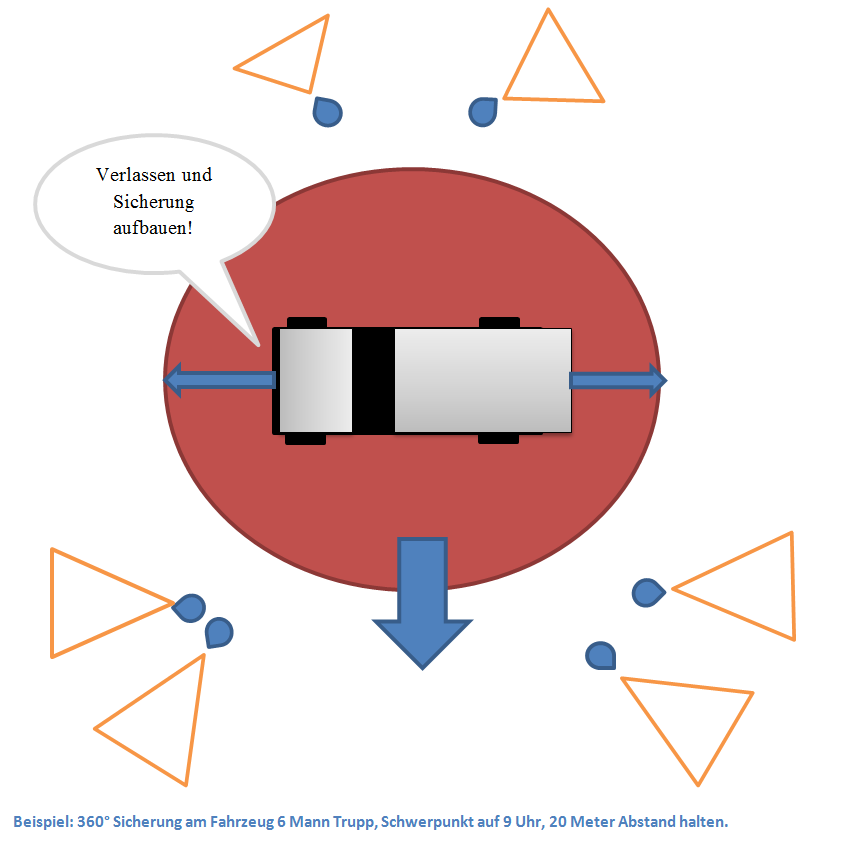
\includegraphics[width=15cm]{../img/basic/fahrzeug/fahrzeug_verlassen}
	\caption{Absitzen und Sicherung beim Fahrzeug}
\end{figure}


\pagebreak
\section{Erste Hilfe}
Grundsätzlich gilt auch in Arma: \textbf{Eigenschutz geht vor Fremdschutz!}. Bevor ihr eurem Buddy oder einem Kameraden helft, stellt sicher, dass ihr dies auch gefahrlos tun könnt! Ansonsten liegt noch jemand verwundet in der Gefahrenzone!\\
Folgende Schritte sind zu tun:
\begin{enumerate}
	\item Sichern und Bergen des Verwundeten (Rauchgranaten einsetzen!)\\
			Eigenschutz geht vor! Erst die Umgebung sichern, dann den Verletzten bergen! 
	\item Bewusstsein und Puls checken (ggf. CPR anwenden lassen!)
	\item Verletzungsgrad feststellen
	\item \textbf{Melden: Verletzungsgrad, Position, weitere Angaben!}
	\item Blutungen stillen! (Gliedmaßen abbinden, Verletzungen versorgen)
	\item ggf. Sanitäter/MedEvac anfordern
	\item Patienten stabil halten, bis Sanitäter eintrifft oder Patient transportiert werden kann.
	\item Falls nötig, Patient verlegen
\end{enumerate}
Den Anweisungen des Sanitätspersonals ist Folge zu leisten! Falls nötig, ist der Patient selbstständig zu einer Verwundetensammelstelle zu verlegen.
Zur Veranschaulichung oder zum Ausdruck kann folgendes Flussdiagramm behilflich sein.
%TODO grafik erneuern
\begin{figure}[htbp]
		\centering
			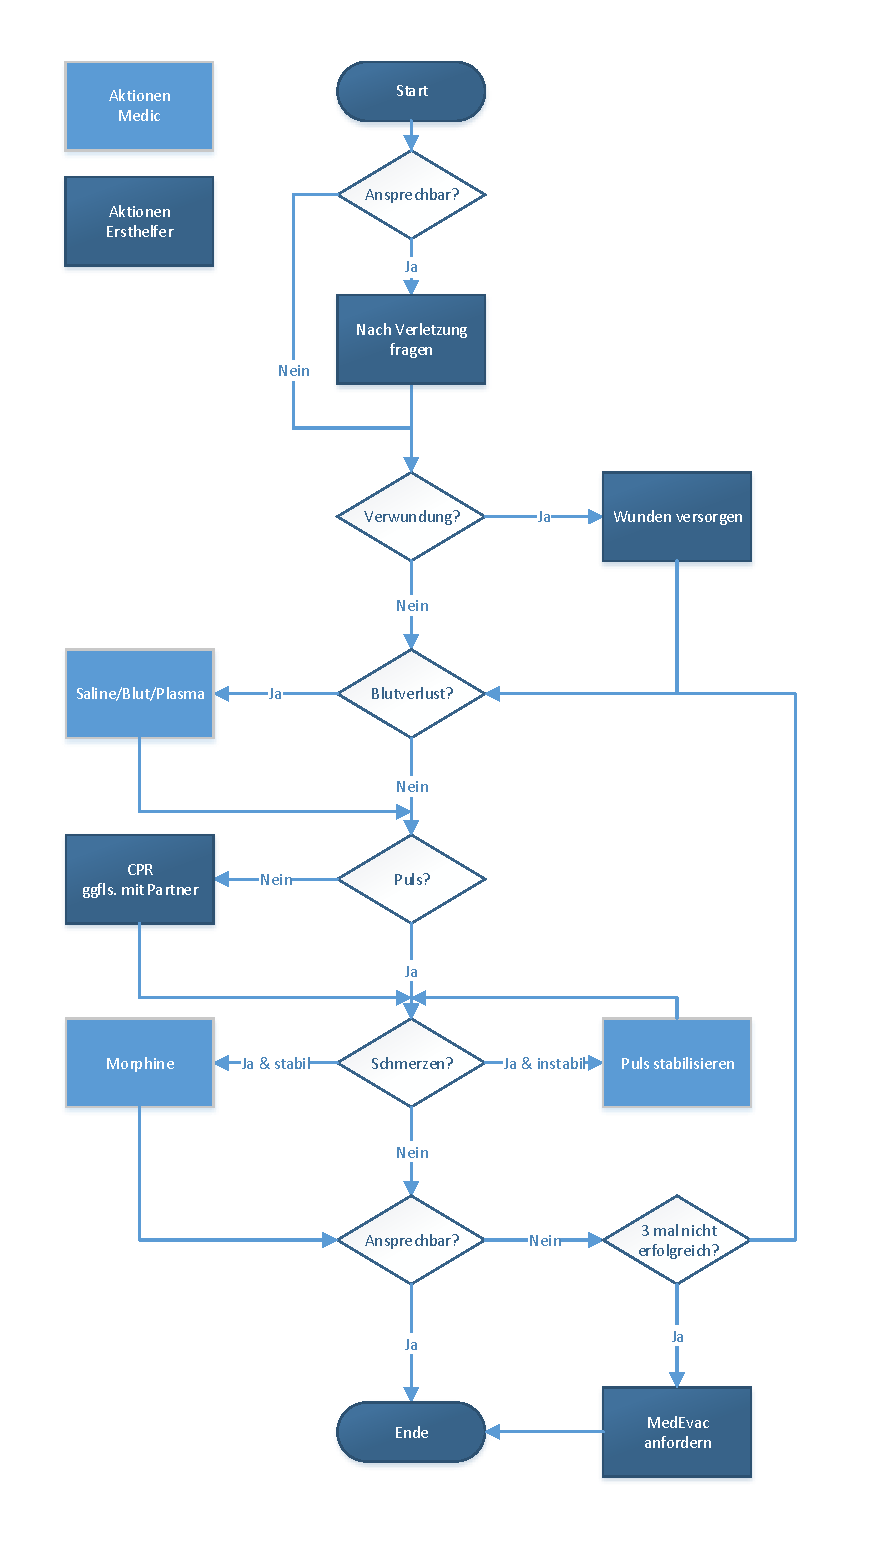
\includegraphics[width=1\linewidth]{../img/basic/erste_hilfe/ersthelfer}
			\caption{Erste Hilfe im TTT}
\end{figure}

\pagebreak
\section{Verhalten bei Feindkontakt}
Wird ein Feind ausgemacht, so meldet ein Truppmitglied diesen an den TF.\\

Dies könnte im Truppfunk so gemeldet werden:\\
>>1 hier 6, Kontakt, stationäres MG auf 290°, Entfernung ca. 800\,m, Kalt<<

Eine andere Situation ergibt sich wenn der Feind das Feuer auf die eigene Stellung eröffnet. Hier hängt es von der Ausgabe des Feuerstatus ab. Ist Feuerstatus rot ausgegeben wird das Feuer nur erwidert wenn es ums blanke überleben geht.\\

Hier kommen die Kommandos >>Stellung wechseln<<, >>Feuer Frei<<, >>Ausweichen<< oder >>Verzögern und Ausweichen<< in Frage.\footnote{Ausführlich in >>\nameref{sec:kommando}<< beschrieben}\\

In allen fällen gibt der TF das Kommando aus, wie sich verhalten werden soll.

%Fortgeschrittenes
\part{Erweiterte Kenntnisse}
%TODO Kurze Beschreibung
\vspace{-5mm}
\chapter{Führen}
\section{Der Befehle}
\label{subsec:befehl}
\begin{quote}
	\glqq Richtig ist besser\grqq
\end{quote}
Befehle sind laut Lehrbuch eine „Anweisung zu einem bestimmten Verhalten, die ein Vorgesetzter einem Untergebenen mit dem Anspruch auch Gehorsam erteilt“. Bei uns einfach „Mach dies und das und möglichst zum Zeitpunkt X“. Der Befehl ist in der Regel ein Gespräch bei uns zwischen Befehlsgeber und Befehlsempfänger. Der Befehl enthält einen Auftrag.\par
Der Auftrag ist das Kernstück und enthält die Informationen, auf die es ankommt.

\paragraph*{Befehle sind verbindlich!}
Befehle des „Vorgesetzten“ sind während der Mission umzusetzen, außer sie basieren auf fataler Fehleinschätzung aufgrund mangelnder Informationen, die dem Vorgesetzten nicht vorliegen. Dann gilt: Vorgesetzen informieren (beispielsweise über Feindkräfte, Lage, mangelnder Ausrüstung) und neue Befehlsausgabe abwarten. Absolut zu vermeiden sind Diskussionen. Dafür haben wir eine Nachbesprechung, wo alle Fehler und Fehlentscheidungen besprochen werden können. Weiterhin hat eine schlichte Befehlsverweigerung gewisse Konsequenzen.

\paragraph*{Befehle sind kurz und präzise!}
Richtig Befehle auszugeben ist für uns Spieler nicht einfach. 
Neben den vielen „öhm, ehm“ kommt besonders über Funk gerne mal kompletter Unsinn aus dem eigenen Mund. 
Weil wir erst während dem sprechen unsere Gedanken sortieren. 
Daher gilt „erste denken, dann sprechen“ und für Funksprüche „erst denken, drücken, sprechen“. Lieber ein paar Sekunden warten, konzentrieren, sortieren und dann die Befehlsausgabe.
Im folgenden bekommt wird der Aufbau des Befehls erläutert. Regel Nr.1: Konzentriert euch auf die Information, lasst den Schnickes und blümerante Dinge weg.
Faustregel zur Länge: Bleibt kurz und präzise. Floskeln weglassen -- und lieber später mal den Kameraden für die gute Umsetzung loben. 

\paragraph*{Möglicher Aufbau eines Befehls}
\begin{enumerate}
	\item Vorwarnung
	\item Rückmeldung
	\item Kurze Beschreibung der Situation (optional)
	\item Auftrag
	\item Auftragsbestätigung
	\item Auftragsauslösung
\end{enumerate}

Beispiel eines Befehls:
\begin{enumerate}
	\item ZF: >>Trupp Rot, bereit machen, neuer Auftrag in 1 Minute!<<
	\item TF: >>Trupp Rot bereit!<<
	\item ZF: >>Trupp Rot, aufgepasst: Lage und Vorhaben: Wir müssen im Dorf Kabalis eine Stellung errichten, dazu wollen wir ein Gebäude einnehmen. Trupp Blau wird den Vorstoß von der jetzigen Stellung hier absichern. Trupp Rot wird das Haus einnehmen. Wir erwarten nur leichten Widerstand -- evtl. ein paar verstreute Infanteristen in der Umgebung. So verstanden?<<
	\item TF: >>So verstanden!<<
	\item ZF: >>Trupp Rot, Euer Auftrag: Einnehmen des weißen, flachen Gebäudes mit rotem Dach auf 320 Grad, 200 Meter entfernt! Verstanden?<<
	\item TF: >>Verstanden, Einnehmen des weißen, flachen Gebäudes mit rotem Dach auf 320 Grad, 200 Meter entfernt.<<
	\item ZF: >>Gut, ausführen wenn bereit!<< (Truppführer entscheidet Zeitpunkt)\\ 
	ZF: >>Gut, sofort ausführen!/ Ausführen bei Erreichen des Punktes X, Ausführen bei 0815 Ortszeit<< (Zugführer entscheidet, wann und wo).
	\item ZF: >>Meldung bei Vollzug!<<
\end{enumerate}

\section{Der Auftrag}
\label{subsec:auftrag}
	Beispielhafter Aufbau eines Auftrags:\par
	In oben genanntem Beispiel ist folgender Auftrag zu finden:
	\begin{hint}
		Trupp Rot, Euer Auftrag: Einnehmen des weißen, flachen Gebäudes mit rotem Dach auf 320 Grad, 200 Meter entfernt! Verstanden?<<
	\end{hint}
	Der Auftrag kommt mit dem Kommando >>Einnehmen<< (siehe \ref{sec:kommando}). Nach dem Kommando kommt das Ziel, welches eingenommen werden soll. Danach noch Richtung und Entfernung, damit der Auftragsempfänger auch das einnimmt, was der Auftragsgeber meint. Das Ganze übersichtlich dargestellt:
	\begin{enumerate}
		\item Kommando
		\item Ziel
		\item Ortsangabe (Richtung \& Entfernung)
	\end{enumerate}

\subsection{Auftragstaktik}\hfil
	\begin{quote}
		\glqq Auftragstaktik Baby! Im \ac{TTT} arbeiten wir mit Aufträgen -- nicht mit der Hundeleine.\grqq
	\end{quote}
	Gute „Führer“ arbeiten IMMER auftragsbasiert -- also eine dezentrale Befehlsausgabe mit Vertrauen, dass der Auftragsempfänger den Auftrag selbständig im Sinne des Befehls erledigt. Man gibt als einen Auftrag – aber NICHT wie dieser Auftrag erreicht wird. Es kann dem Zugführer in der Regel völlig egal sein, über welchen Eingang das Haus genommen wird. Auftrag erteilen und alles Weitere dem Truppführer überlassen, er kann das am besten entscheiden, wie er seine Leute sicher und erfolgreich ins Haus bekommt.
	\par\medskip
	Das Gleiche gilt für Truppführer: Hört auf mit dem Mikromanagement! Wenn ihr Eurem Trupp das Kommando gebt >>Deckung<< dann muss nicht gesagt werden, hinter welchen Felsen das jetzt sein soll. Dass gleiche gilt für „Stellung“ – der Trupp wird automatisch Stellung beziehen und bei Erfolg den Vollzug durchgeben. Wenn ein Truppführer einen Auftrag erteilt, beispielsweise ein Kontakt zu bekämpfen, dann geht das folgendermaßen:
	\begin{longtable}{P{0.95\linewidth}}
		\toprule
		TF: >>5-6, 2 Feindkräfte auf 120 Grad, 200 Meter, am Spitzbaum, gesichtet?<<\\
		\rcg TM 6: 5-6: >>Gesichtet!<<\\
		TF: >>5-6, Stellungswechsel, dann bekämpfen, Meldung bei Vollzug!<<\\
		TF: >>Feuer frei!<< (Feuerfreigabe)\\
		\bottomrule
	\end{longtable}		
	
5 und 6 haben ihren Auftrag: Sie suchen sich eine geeignete Stellung mit genügend Deckung, überprüfen kurz die Flanken (rechts und links), sprechen sich kurz ab, legen Feuermodus fest und feuern nach Absprache untereinander. Danach melden Sie dem TF per Funk das erfolgreiche bekämpfen des Gegners. Anschließend verlegen sie zurück in Ausgangsstellung. 
%\section{Führen als Operationsleitung}
%\section{Führen als Zugführer}
%\section{Führen als Truppführer}
\chapter{Unterstützung anfordern}
\section{Logistik und medizinische Unterstützung}
Wie anfänglich erwähnt, umfasst das Aufgabenfeld des FAC die Kommunikation und
Koordination verbündeter Lufteinheiten. Neben dem CAS, welcher das Kernthema dieser
SGA darstellt, beschäftigt der FAC sich im TTT auch mit der logistischen und
medizinischen Versorgung der Bodentruppen. Dabei wird für die medizinische Versorgung,
welche meist in Form einer Evakuierung auftritt der Fachbegriff MEDicalEVACuation
verwendet. Bei logistischer Unterstützung handelt es sich meist um die Lieferung von
Munition, sonstigen Materialen oder das Verlegen von Einheiten. Häufig werden im TTT
für beide Aufgabenbereiche Helikopter verwendet.

\subsection{Der 5-Liner im Detail}
Das TTT wendet für beide Versorgungsarten ein fünfzeiliges Informationsprotokoll an,
welches sich 5-Liner nennt. Folgende Informationen sind dabei enthalten.\\

5-Liner:
\begin{enumerate}
	\item LZ 
	\item Heading
	\item Receiver
	\item Supply
	\item Type Mark
\end{enumerate}

Hier wird noch einmal die Bedeutung der einzelnen Lines im Detail erklärt.
\paragraph*{LZ}\hfil\\
Die LZ ist die Landezone, welche für das versorgende Flugobjekt eingerichtet wird. Der
Fokus liegt dabei auf der Funktionalität und Sicherheit des ausgewählten Gebietes.
\paragraph*{Heading}\hfil\\
Der Heading ist die Anflugrichtung, aus der sich das Flugobjekt der LZ nähert. Da im
Gegenteil zum CAS kein IP existiert, wird hier mit oberflächlichen Angaben, d.h.
Himmelsrichtungen gearbeitet.
\paragraph*{Receiver}\hfil\\
Der Receiver ist der Empfänger der Versorgung, dabei werden Truppfarben verwendet.
Der Empfänger ist ebenfalls für die Sicherung und Einrichtung der Landezone zuständig.
\paragraph*{Supply}\hfil\\
Supply beschreibt die Art der Versorgung. Im Falle von Materialien wie z. B. Munition wird
erst der Materialtyp und anschließend die benötigte Anzahl genannt. Sollten mehrere
Güter benötigt werden, wird nach Abschluss des ersten Materials erneut Typ und Anzahl
des zweiten Materials genannt. Hier noch einmal im Muster verdeutlicht.
\begin{hint}
\,[Material A], [Anzahl Material A] sowie [Material B], [Anzahl Material B] etc.
\end{hint}
Sollte es sich bei einem logistischen Auftrag um Verlegung von Truppen handeln, wird
nach folgendem Muster verfahren.
\begin{hint}
Verlegung von [Truppname] nach [Zielort (LZ)]
\end{hint}
Bei einer medizinischen Evakuierung wird der Medevac über die Art des Einsatzes, die
Anzahl der Verwundeten sowie ihren Status informiert. Auch hierzu ein Musterbeispiel.
\begin{hint}
Medevac, 1 Verwundeter, Status gelb.
\end{hint}
Sollte es sich um mehrere Verletzte handeln, wird der Status nicht einzeln angegeben,
sondern verallgemeinert.
\begin{hint}
Medevac, 2 Verwundete, Status rot.
\end{hint}
\paragraph*{Type Mark}\hfil\\
Type Mark beschreibt, ähnlich wie beim 9-Liner, die Markierung des Ziels. Im Falle von
Logistik und Medevac handelt es sich dabei aber um die angepeilte Landezone. Auch hier
sind wie bei CAS Rauch, Laser oder Lichtsignale eine Möglichkeit.

\pagebreak
\section{Close Air Support anfordern}
	Zu den Aufgabenspektrums einen Funkers im TTT gehört auch die Anforderung von Luftnahunterstützung, wie diese zu planen und umsetzten ist, wird im folgenden Kapitel behandelt.
\subsection{Die Plaungunsphase}
	Die Planungsphase ist der erste und wichtigste Schritt für erfolgreichen CAS. Der FAC verschafft sich einen Überblick über die zur Verfügung stehenden Mittel. Dabei überlegt er, was er genau erreichen will und wie er es am Besten umsetzen kann. Wichtige Faktoren dabei sind Positionen verbündeter oder ziviler Kräfte, sowie Einschränkungen durch Gelände oder Feind (z.\,B. Hügel, Flugabwehr, etc.).
	\par\medskip
	Die drei W's:\\
	\begin{tabular}{ll}
	\textbf{Wer} &  steht mir zur Verfügung?\\ 
	\textbf{Was} &  will ich erreichen?\\ 
	\textbf{Wie} &  kann ich es am Besten umsetzten?\\ 
	\end{tabular} 

\paragraph*{Check-in Briefing}
	\begin{quote}
		\glqq Wer steht mir zur Verfügung?\grqq
	\end{quote}
	Diese Frage lässt sich mit einem einfachen Protokoll abfertigen, dem >>Check-in Briefing<<. Dieses Protokoll wird in der Anfangsphase einer Mission, von Pilot und FAC, über Funk abgearbeitet. Der FAC hat dadurch eine genaue Vorstellung welche Arbeitsmittel ihm zur Verfügung stehen. Das Check-in Briefing besteht aus folgenden Informationen:
	\begin{itemize}
		\item Typ des CAS"=Objektes
		\item momentane Position
		\item Bewaffnung
		\item Verfügbarkeitszeitraum
	\end{itemize}

\paragraph*{Was will ich erreichen und wie kann ich es am Besten umsetzen?}
	Neben den neun namensgebenden Informationen des 9-Liners, muss auch der Typ des
	Angriffs bestimmt werden. Dabei wird zwischen drei Arten unterschieden.
	Bei einem Typ 1 Angriff, welcher in den meisten Fällen genutzt werden sollte, haben
	sowohl FAC, als auch das Flugobjekt Sicht auf das Ziel und zueinander.
	Der Typ 2 Angriff deckt mehrere Fälle ab. Hierbei können ein oder mehrere Optionen
	zutreffen:
	\begin{itemize}
		\item CAS sieht Ziel nicht
		\item FAC sieht Ziel nicht
		\item FAC sieht CAS nicht
	\end{itemize}
	Ein Typ 3 Angriff verhält sich von den Parametern ebenfalls wie der Typ 2 Angriff. Dabei
	darf das Flugobjekt Ziele eigenständig bekämpfen, welche sich in der vom FAC
	angegebenen Zielbereich befinden.\par
	Für die Kernplanung ist es wichtig, dass der FAC seine CAS"=Maschine kennt, damit er im
	Bereich des Möglichen plant. In die Planung des Angriffs spielen viele Faktoren ein, wie
	z.\,B. Anflugschneise, verbündete Kräfte, Bewaffnung, Feindtyp, etc. Hat der FAC die
	Planung des Angriffs beendet, gibt er diese in Form eines Protokolls über Funk durch.
	Dieses Protokoll wird auch >>9-Liner<< genannt. Das Fomular deckt alle wichtigen
	Informationen ab, damit der Pilot erfolgreich CAS fliegen kann. Folgende Informationen
	sind in einem 9-Liner enthalten.

\subsubsection{9-Liner}
	\begin{itemize}
		\item IP/BP
		\item Heading
		\item Distance
		\item Elevation
		\item Description
		\item Location
		\item Typ Mark
		\item Friendlies
		\item Egress
	\end{itemize}
	Hier wird noch einmal die Bedeutung der einzelnen Lines im Detail erklärt.
\paragraph*{IP\,/\,BP}
	Der Initial-Point ist der Ausgangspunkt des 9-Liners. Auf diesem Ausgangspunkt bauen
	alle weiteren Informationen auf. Das Flugobjekt fliegt zuerst diesen Punkt an und führt
	nach gegebenen Informationen den Einsatz aus.
	Die Battleposition ist eine Kampfzone für Helikopter, von der aus der Helikopter den CAS"=Auftrag ausführt.
\paragraph*{Heading}
	Der Heading bezeichnet die Sicht-, Bewegungsrichtung an der sich das CAS"=Objekt
	orientieren muss. Hierbei wird mit Gradzahlen gearbeitet. Der Offset ist dabei optional
	dieser wird z.\,B. bei besonderen Gefahrensituationen eingesetzt.
\paragraph*{Distance}
	Bezeichnet den Abstand, welche sich zwischen IP und Ziel befindet.
\paragraph*{Elevation}
	In der Line \textit{Elevation} wird die Höhe angegeben, auf der sich das Ziel befindet.
\paragraph*{Description}
	Bei der \textit{Description} handelt es sich um eine kurze Zielbeschreibung für den Piloten. Er kann sich dadurch besser auf sein zugewiesenes Ziel einstellen.
\paragraph*{Location}
	Die \textit{Location} ist das Grid, auf dem sich das Ziel befindet.
\paragraph*{Typ Mark}
	\textit{Type Mark} beschreibt die Markierung des Ziels. Möglichkeiten hierbei sind z.\,B. Rauch, Laser, oder keine Markierung.
\paragraph*{Friendlies}
	\textit{Friendlies} gibt an, ob und wo sich verbündete Kräfte aufhalten. Diese können sich optional auch mit z.\,B. grünem Rauch markieren. Ist der CAS"=Angriff mit >>Danger Close<< betitelt, wird die Markierung eigener Truppen zur Pflicht.
\paragraph*{Egress}
	Der Egress bestimmt die Abflugrichtung des Flugobjekts. Ist z.\,B. der Luftraum hinter dem Ziel nicht aufgeklärt, kann es unmöglich durch diesen Bereich abdrehen und zur IP zurückkehren.

\subsection{Die Aktionsphase}
	Nachdem der Liner über Funk an den Piloten übermittelt wurde, beginnt die Aktionsphase. Der Pilot beginnt mit der Ausführung der Befehle.\par
	Gehen wir von einem 9-Line-Briefing aus, bei dem der Pilot den 9-Liner bereits ausgewertet hat und bei der IP auf Standby steht. Ab der IP, dem Zentrum des Briefings beginnt der Angriff. Damit Pilot und FAC Anhaltspunkte über den Status des CAS haben, gibt es 3 kurze Meldungen an Schlüsselpunkten des Angriffs.\par
	Die erste Meldung gibt der Pilot bei Erreichen der IP durch:
	\begin{hint}
	Reaper inbound, kommen.
	\end{hint}
	Der FAC hat hier zwei Optionen. Entweder die Bestätigung zur weiteren Ausführung nach Plan oder eine letze Abbruchchance. Zum Bestätigen des Angriffs wird >>Continue<< und zum Abbruch des Angriffs >>Abort<< verwendet.\par
	Gehen wir davon aus der Pilot bekommt das >>Continue<<. Laut Liner wurde das Ziel mit rotem Rauch markiert. Für den Pilot bedeutet das, dass er sich sobald er Sichtkontakt zum Ziel hat, beim FAC mit >>Spot<< melden muss. Sollte er das Ziel nicht erkennen ist >>No Spot<< zu verwenden, wenn letzeres eintritt dreht der Pilot ab. Keinesfalls schießt er nach Vermutung.\par
	In unserem Beispiel gehen wir wieder davon aus, dass der Pilot >>Spot<< durchgibt. Ist er feuerbereit meldet er >>Tally<<. Darauf muss der FAC ihm schnellstmöglich >>Cleared Hot<< funken, da der Pilot noch keine Feuerfreigabe hat. Sollte der Pilot das Ziel erfasst haben, jedoch kein >>Cleared Hot<< hören, dann isSpott der Angriff abzubrechen und über die Abflugszone zurück zur IP zu fliegen. Kommt es vor, dass der Pilot das Ziel sieht, aber aus Gründen nicht feuerbereit ist, meldet er >>No Joy<<. Nach dem Angriff meldet der FAC je nach Erfolg >>Hit<< oder >>Miss<<, um den Piloten Feedback zu geben.

\subsection{Anwendung}
	Hier sind noch einmal zwei komplette CAS Beispiele hinterlegt. Die Theorie der letzten Kapitel wird hier angewendet und zum besseren Verständins mit Bildmaterial verdeutlicht.

\paragraph*{Check-In Briefing}
	Da sich noch keine Gelegenheit ergeben hat, klinkt sich der FAC auf die Frequenz von Reaper (Jet) und verlangt von ihm ein Check-in Briefing.
	\begin{longtable}{P{0.95\linewidth}}
	\toprule
	Grau meldet sich auf Funkfrequenz an, Reaper hier Grau, kommen.\\
	\rcg Reaper hört, kommen.\\
	Reaper, Anfrage auf Check-in Briefing, kommen.\\
	\rcg Reaper bestätigt, Check-in Briefing lautet wie folgt. 1x A10 Thunderbolt II. Altis Airport.
	Gau-8 30mm 1000x, GBU-12 4x, Hydras 14x, Maverickraketen 2x, Sidwinderraketen 2x,
	TOS 10 Minuten.\\
	Grau bestätigt Check-in Briefing, melde mich bei Bedarf, Ende.\\
	\bottomrule
	\end{longtable}

\paragraph*{Helikopter-CAS}
	Wir gehen von bereits abgeschlossenem Check-in Briefing aus. Grau hat einen Panzer
	aufgeklärt. Der Trupp will, dass Adler den Panzer mit einem Kampfsprung ausschaltet,
	dazu benutzen sie einen 9-Liner.\par
	\textit{Grau arbeitet den 9-Liner aus und klinkt sich auf die Frequenz von Adler. Der Trupp plant
	das Ziel mit Laser zu markieren, sodass Adler aufsteigen kann, den Laser aufschaltet und
	eine Hellfirerakete abfeuert, um dann sofort wieder abzutauchen.}
	\begin{longtable}{P{0.95\linewidth}}
	\toprule
	Grau meldet sich auf Funkfrequenz an, Adler hier Grau, kommen.\\
	\rcg Adler hört, kommen.\\
	Adler bereit für 9-Liner, kommen?\\
	\rcg Adler bestätigt, bereit für 9-Liner, kommen.\\
	Grau verstanden, 9-Liner lautet wie folgt. Typ 1 Angriff, BP Alpha, Heading SO xxx Grad,
	Distance x m, Description 1x MBT, Location xxx-xxx (Koordinate), Typ Mark Laser,
	Friendlies xxx m N, Egress NW Remarks, es wird mit Kampfsprüngen gearbeitet,
	lasergelenkter Raketenangriff. So verstanden, kommen?\\
	\rcg Adler bestätigt 9-Liner, Location xxx-xxx (Koordinate), Friendlies xxx m Nord, kommen.\\
	Grau bestätigt, melden wenn bei BP Alpha.\\
	\rcg \textit{Adler bewegt sich im Tiefflug zu BP Alpha, um nicht aufgeklärt zu werden. Nach Erreichen des BP meldet Adler sich wieder bei Grau.}\\
	\rcg Grau hier Adler, kommen.\\
	Grau hört, kommen.\\
	\rcg Adler bei BP Alpha, bereit für Kampfsprung, Laser on, kommen.\\
	Grau bestätigt, bereit für Kampfsprung, lasing, kommen. \textit{Grau schaltet den Laser an.}\\
	\rcg Adler bestätigt, lasing, Sprung auf Befehl.\\
	Hier Grau, Sprung!\\
	\rcg \textit{Adler führt einen Kampfsprung aus.}\\
	\rcg Spot!\\
	\rcg \textit{Adler erfasst den Laser.}\\
	\rcg Tally!\\
	Cleared Hot!\\
	\rcg Feuerfreigabe durch Grau, Adler schießt die Rakete ab. Einschlag der Rakete ins Ziel.\\
	Hit!\\
	\rcg Adler taucht ab.\\
	\rcg \textit{Adler taucht wie besprochen wieder hinter die Bergkuppe ab.}\\
	\bottomrule
	\end{longtable}

\paragraph*{Jet-CAS}
	Ausgangslage: Grau soll dem Zug bei der Einnahme einer Stadt zuarbeiten. 
	Der Auftrag ist die Deaktivierung eines Funkturms, um die Kommunikation des Feindes zu schädigen. Der Funkturm wird u.a. von einem schwer gepanzerten Fahrzeug bewacht. 
	Nach Anfrage hat Gelb Grau CAS Freigabe erteilt.
	\par\medskip
	Als Check-In Briefing wird das oben aufgeführte Beispiel genannt.\par
	Grau macht sich jetzt daran, den 9-Liner auszuarbeiten, um sich danach bei Reaper zu
	melden das wird überflüssig, sollte schon eine Taskforce gebildet sein. Nach
	abschließender Planung des FACs, meldet er sich wieder auf der Frequenz von Reaper.
	\begin{longtable}{P{0.95\linewidth}}
	\toprule
	Grau meldet sich auf Funkfrequenz an, Reaper hier Grau, kommen.\\
	\rcg Reaper hört, kommen.\\
	Reaper bereit für 9-Line Briefing, kommen?\\
	\rcg Reaper bestätigt. Bereit für 9-Line Briefing, kommen.\\
	Grau verstanden, 9-Line Briefing lautet wie folgt.Typ 2 Angriff, IP Romeo, Heading Süden xxx Grad, Distance x,x klicks, Elevation xx m, 1x MBT, Location xxx-xxx (Koordinate), Typ Mark roter Rauch,  Friendlies x, x klicks Nordwest, Egress NW, Remarks: Waffeneinschränkungen: GBU-12 So verstanden Reaper, kommen?\\
	\rcg Reaper bestätigt, Ziel auf xxx-xxx (Koordinate), Verbündete xxx m NW, kommen.\\
	Grau bestätigt, melden bei IP Romeo.\\
	\rcg \textit{Reaper wertet den 9-Liner aus und beginnt mit dem Anflug, jetzt beginnt die Aktionsphase. Zwei Minuten später, erreicht Reaper IP Romeo und meldet sich bei Grau.}\\
	\rcg Reaper inbound, kommen.\\
	Continue, lasing.\\
	\textit{Grau schaltet Laser ein}\\
	\rcg Spot. \textit{Reaper nimmt den Lasermaker auf den Radar war}\\
	\rcg Tally. \textit{Reaper ist unmittelbar vor dem Angriff und bekommt Sichtkontakt auf das Ziel bzw. den Leitlaser für die lasergelenkte Bombe.}\\
	Cleared Hot.\\
	\rcg \textit{Einschlag der Bombe, dass Ziel wurde getroffen}\\
	Hit, Standby auf IP Romeo, kommen.\\
	\rcg Bestätige Hit, Abflug xxx, Standby auf IP Romeo.\\
	\bottomrule
	\end{longtable}
\section{Artillerie}
Das Konzept der Artillerie befindet sich im Moment noch in Arbeit und wird in einer späteren Version des Handbuches hinzugefügt.
\pagebreak
\chapter{Close Quarters Battle}
\label{CQB}
\subsection{Technik: Zweier-Haken}
\begin{center}
	Modified Button hook
\end{center}
\begin{enumerate}
	\item Aufstellung Rechts und Links von der Tür (Türangeln beachten)
	\item Gleichzeitiger, überraschender Eintritt als Zwei-Mann-Team \\
		Feuerbereiche überlappen sich
	\item Zwei Mann laufen entlang der Wand, um etwaige Gegner in den Ecken zu bekämpfen
	\item Zwei Mann nehmen Sicherungsposition ein und bereiten sich auf weiteres Vorgehen vor
 \end{enumerate}        
 Vorteile
 \begin{itemize}
	 \item Sehr schnelles, einfaches Eindringen
	 \item Ideal für größere Räume oder Innenhöfe
	 \item Einfaches Manöver, auch für Anfänger geeignet
	 \item Überlappender Feuerbereich im Eingang
	 \item Für innen öffnende Türen ideal
 \end{itemize}     
  Nachteile
  \begin{itemize}
  	\item Tür / Eingang muss breit genug sein für nahezu gleichzeitiges Eindringen
  	\item Tür / Eingang muss vorher überquert werden (Überraschungseffekt)
  	\item Wenn die Tür sich nach außen öffnet, wird das gleichzeitige Eindringen erschwert. Team muss daher die Startposition anpassen
  \end{itemize}          
\subsection{Technik: 4-Mann-Zweier-Haken}
\begin{center}
	modified button hook -- Variante bei der Buddy-Teams erhalten bleiben
\end{center}
	\begin{enumerate}
		\item Aufstellung Rechts und Links von der Tür (Türangeln beachten) \\
		Klare Sektorenvergabe (links und rechts)
		\item Gleichzeitiger, überraschender Eintritt als 2-Mann-Team \\
		Feuerbereiche überlappen sich \\
		Eintrittsrichtung Beispiel: \\
		Nr.1 + 2: links; Nr. 3 + 4: rechts
		\item Vier Mann laufen entlang der Wand um etwaige Gegner in den Ecken zu bekämpfen
		\item Vier Mann nehmen Sicherungsposition ein und bereiten sich auf weiteres Vorgehen vor
	\end{enumerate}      
\subsection{Technik: 4-Mann-Fluten}
\subsection{Technik: Annähern an Gebäude -- Raupe}
\subsection{Technik: High-Low}
\subsection{Technik: Aufstellung Flashbang}
%\pagebreak
\chapter{Hubschrauber für Infanteristen}
\label{HuFIn}
\section{Hubschrauber}
	Helikopter können sehr vielseitig eingesetzt werden. Sie können Gebiete großflächig aufklären, Truppen und Güter transportieren, Personen in Not helfen und vieles mehr. Damit diese Einsätze so schnell und leicht wie möglich ohne viel Aufwand abgewickelt werden können, gibt es einige Hilfsmittel und Richtlinien. Nachfolgend werden die gängigsten Helikoptertypen im TTT näher erklärt. 
\subsection{Modellübersicht}
\paragraph*{UH-60 Blackhawk}
	\begin{itemize}
		\item 4 Mann Besatzung (2 Piloten, 2 Gunner); 12 Infanteristen 
		\item 2x 7,62mm Minigun 
		\item 168 Täuschkörper in Mehrfachwurf (24 Stück) oder automatisch (2 Stück pro 
		Sekunde, 8 Sekunden lang) 
	\end{itemize}
\paragraph*{CH-47 Chinook}
	\begin{itemize}
		\item 4 Mann Besatzung (2 Piloten, 2 Gunner); 24 Infanteristen 
		\item 2x 7,62mm Minigun 
		\item 168 Täuschkörper in Mehrfachwurf (24 Stück) oder automatisch (2 Stück pro 
		Sekunde, 8 Sekunden lang) 
	\end{itemize}

\section{Allgemein}
\subsection{Verhalten außerhalb}
	\begin{itemize}
		\item Bei Helikoptern mit seitlichem Aufstieg hat sich die Infanterie frontal dem  
		Hubschrauber zu nähern, um dann in einem Bogen seitlich aufzusteigen. Somit hat 
		die Besatzung jederzeit Blickkontakt.  
		\item Wenn man mit einem bewaffneten Luftfahrzeug operiert, ist jederzeit genug Abstand 
		zu den Waffensystemen zu halten LEBENSGEFAHR
		\item Bei Hanglage ist auf die Rotoren zu achten, da diese, bedingt durch die Schräglage  
		des Fahrzeuges, dem Boden äußerst nahe kommen und somit schwerste 
		Verletzungen anrichten können. 
		\item Immer gilt: Anweisungen der Crew sind Folge zu leisten! Das letzte Wort hat immer  
		der Pilot! 
	\end{itemize}
\subsection{Verhalten innerhalb}
	Die truppinternen Gespräche der Infanterie sollten sich im Helikopter auf ein Minimum reduzieren. Wenn Funkabsprachen unausweichlich sind, sollte die Lautstärke von TFAR auf “Whispern” eingestellt werden, sodass die Helikopterbesatzung ungestört ihrem Dienst nachkommen kann.\par
	Aufgabe der Infanterie im Flug ist es, nach allen Bedrohungen Ausschau zu halten beispielsweise Gewehrfeuer, Raketenbeschuss oder generelles Mündungsfeuer, Bewegungen von Feinden, Hindernissen oder jeglichen anderen Gefahren für das Fahrzeug. Hierbei sollte der Pilot immer umgehend über diese Bedrohungen informiert werden.

\section{Verlegung von Infanterie}
	Vor Einsatzbeginn sind folgende Fragestellungen zu klären:
	\par\medskip
	\begin{tabular}{ll}
	WO  & ist der geplante Landeraum?\\ 
	WAS  & wird transportiert?\\ 
	WIE  & wird verlegt?\\ 
	WER  & steigt auf?\\ 
	\end{tabular}
	\par\medskip
	Falls es keinen FAC gibt, welcher die Ressource über die OPL beantragt, wählt sich die Nr.2 auf die SR der Helikopterbesatzung ein, um später dem Piloten mitzuteilen, dass alle Teile seines jeweiligen Trupps erfolgreich abgesessen sind. Es wird immer vom Rang niedrigsten beginnend abgestiegen.\par
	Sobald der Pilot den “Touchdown” durchgibt, geht die Befehlsgewalt über die Infanterie wieder an den Truppführer über. Dieser kann nun das eigentliche absteigen befehlen.

\section{Ablaufplan von Extraktion, MedEvac oder Logistik}
\subsection{Anforderung der Ressource}
	Bedingt durch die Einbindung mehrerer Truppteile müssen angeforderte Ressourcen wie MedEvac, Logistik etc. vom Operationsleiter genehmigt werden. Hierzu setzt sich der Forward Air Controller (FAC) mit der OPL in Verbindung und beantragt die Ressource mit Begründung. Der Operationsleiter entscheidet anschließend situationsgerecht und gibt die Ressource entweder frei oder lehnt diese ab. Im Anschluss darauf findet der FAC sich wieder auf seinem eigenen Funkkreis ein, um von der jeweiligen Ressource direkt kontaktiert zu werden. 

\subsection{Landezone finden und einrichten}
	Der FAC verschafft sich in der Zwischenzeit im Einsatzgebiet einen kurzen Überblick über die Topographie und entscheidet im Anschluss darauf, an welcher Position sich im besten Falle die Landezone befindet. Gleichzeitig legt er auch eine sekundäre Landezone für den Notfall fest und markiert beide Positionen entsprechend mit gültiger Beschriftung auf der Karte (siehe hierzu “SGA FAC” von LingLing).\par
	Eine optimale LZ bietet sowohl für den Anflug des Helikopters, als auch für die Infanterie genügend Deckung. Im optimalen Fall sieht der Pilot die LZ schon von weitem bzw. wird frühzeitig über den FAC mittels Landmarke eingewiesen. Die LZ sollte möglichst eben und frei von Hindernissen sein, welche dem Helikopter schaden könnten. Hierbei muss die Größe so gewählt sein, dass genügend Raum für den Helikopter im Landeanflug sichergestellt ist. 
	\begin{figure}[htbp]
		\centering
		\includegraphics[width=0.95\linewidth]{../img/advanced/hubschrauber_+_infanterie/landezone}
	\end{figure}
	\begin{figure}[htbp]
		\centering
		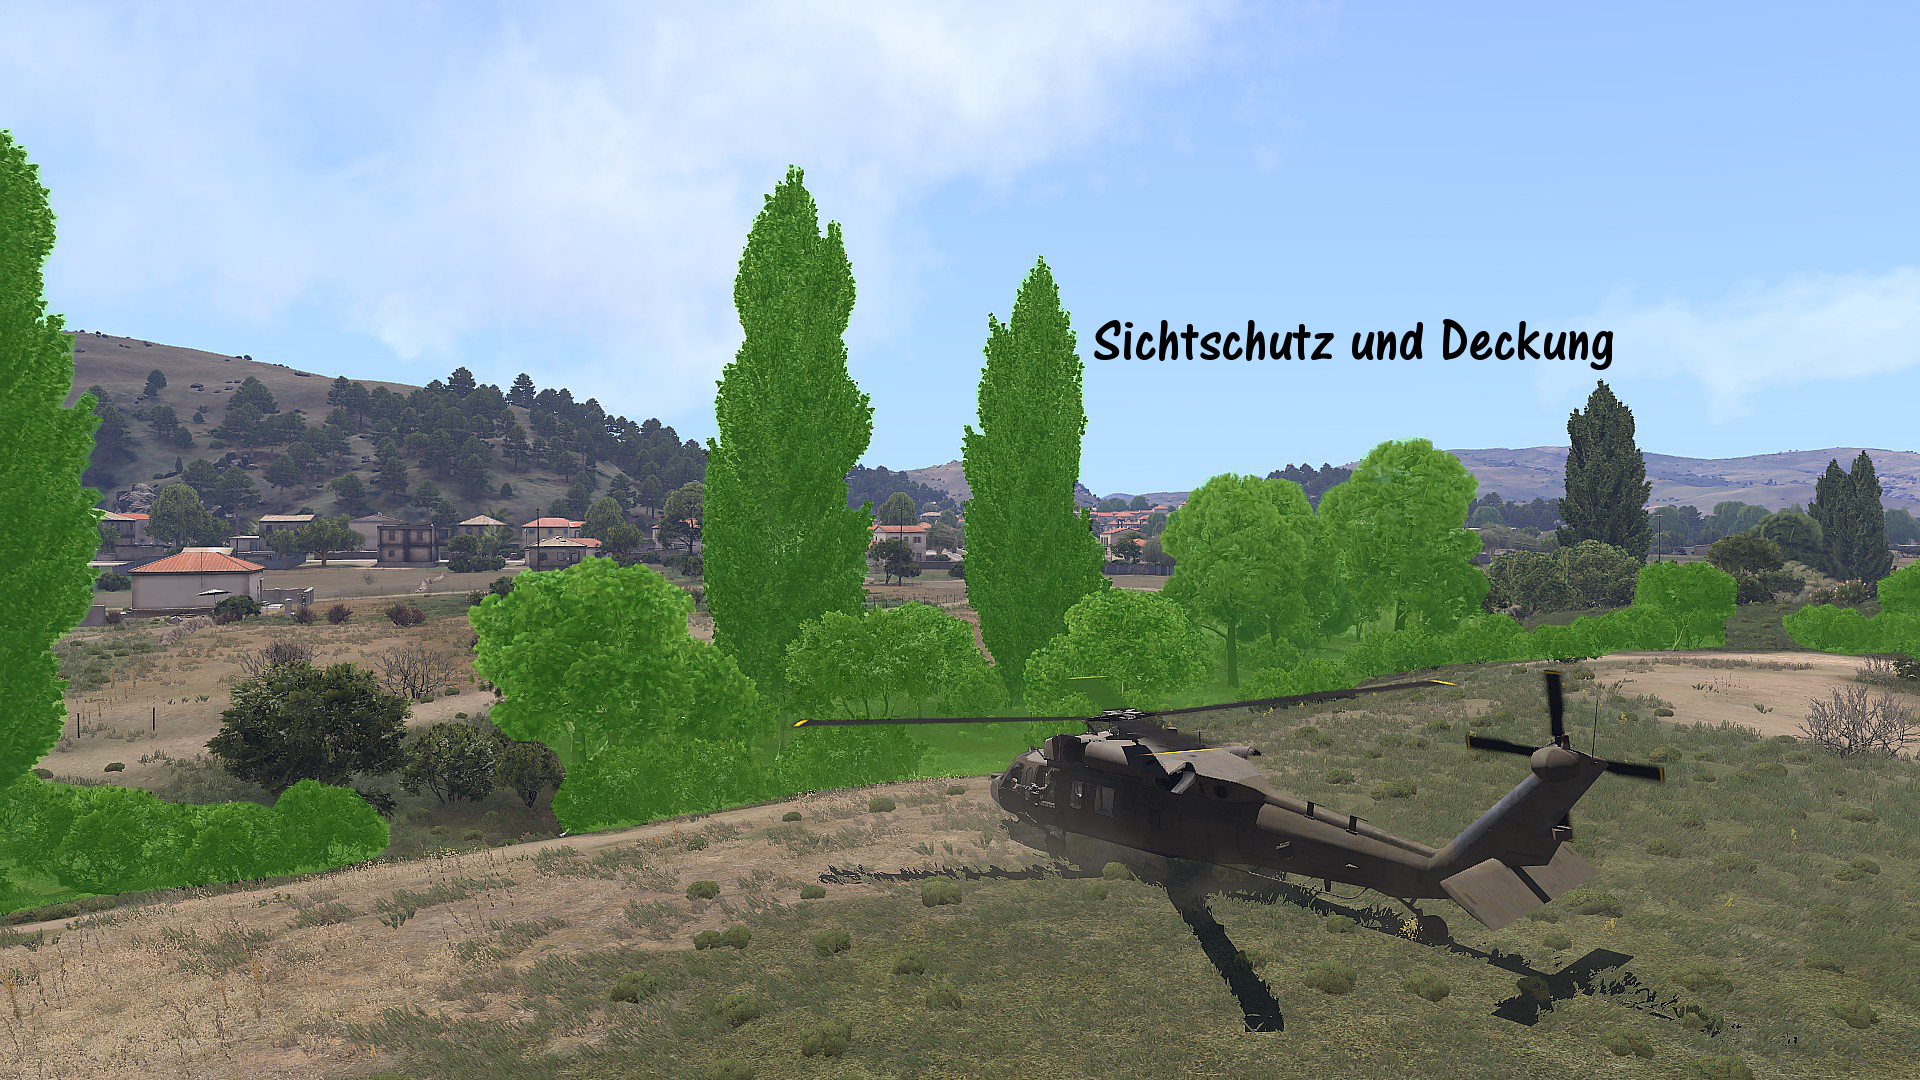
\includegraphics[width=0.95\linewidth]{../img/advanced/hubschrauber_+_infanterie/verdeckte-landung}
	\end{figure}	

\subsubsection{Heiße Landezonen}
	Bei heißen Landezonen kommt es auf eine gute Reaktion der Infanterie und vor allem Schnelligkeit an. Zur besseren Deckung können die Soldaten Rauchgranaten einsetzen, ebenso kann der Pilot das Einrauchen der Landezone befehlen, um die Sichtlinie zu eventuellen Feindkräften zu brechen.\par
	Wenn ein Helikopter eine bereits unter Beschuss stehende Landezone anfliegen soll, ist der Pilot im Voraus darüber zu unterrichten. Da der Pilot zu jedem Zeitpunkt die vollständige Verantwortung über das Luftfahrzeug inkl. Besatzung inne hat, kann dieser zu jedem Zeitpunkt den Anflug abbrechen oder die Landezone verlassen.\par
	Eine Besonderheit stellt das Aufsitzen der Infanterie unter Beschuss dar hierbei wird die normale Aufsitzreihenfolge missachtet, um ein schnelles Aufsitzen der gesamten Kräfte zu ermöglichen.

\subsection{Informationsfluss}
	Die Helikopterbesatzung wird seitens der OPL über die Anforderung der Ressource mit Angabe des Antragstellers informiert. Nach Bestätigung des Auftrags verbindet sich die Besatzung direkt mit dem jeweiligen Trupp und meldet Einsatzbereitschaft. Nun muss der FAC den im Voraus vorbereiteten 5-Liner an die Besatzung übermitteln. Nach erfolgreichem Readback setzt sich der Helikopter in Bewegung und hält ständigen Funkkontakt, um ggf. plötzliche Änderungen oder wichtige Hinweise durchzugeben oder seitens des FACs zu erhalten.
	\par\medskip
	In Sonderfällen kann der FAC die Ressource zunächst in eine Holding Postition beauftragen und im Anschluss, je nach Situationslage, den 5-Liner an die Besatzung übermitteln oder den Einsatz komplett abbrechen.
	\par\medskip 
	Anmerkung: Falls die Verbindung zwischen Helikopter und FAC ausfallen sollte, wählt sich der Pilot selbstständig sofort auf dem SR Kanal des Trupps ein, um eine Funkverbindung wiederherzustellen.

\subsection{Landeanflug - Die Einweisung/ die Übergabe an den Einweiser}
	Der Pilot meldet die Annäherung an den Operationsraum. In diesem Moment geht die komplette Verantwortung zum FAC über. Er befiehlt dem FAC das markieren der Landezone durch Leucht oder Rauchmarkierungen. Der FAC weist auf Anforderung den Piloten in die korrekte Position ein und warnt ihn ggf. über Gefahren.\par
	Tipp: Bei Nacht sieht man sehr gut ein Knicklicht in Kombination mit einer Rauchgranate, welche darauf geschmissen wird.
	\par\medskip
	Sobald der Pilot den “Touchdown” durchgibt darf die Infanterie die nötigen Aufgaben durchführen.\par
	Warum man einen FAC braucht, hier in einem Video verdeutlicht:\\
	\url{https://www.youtube.com/watch?v=NJIZTL2ZyEw}

	\begin{figure}[htbp]
		\centering
		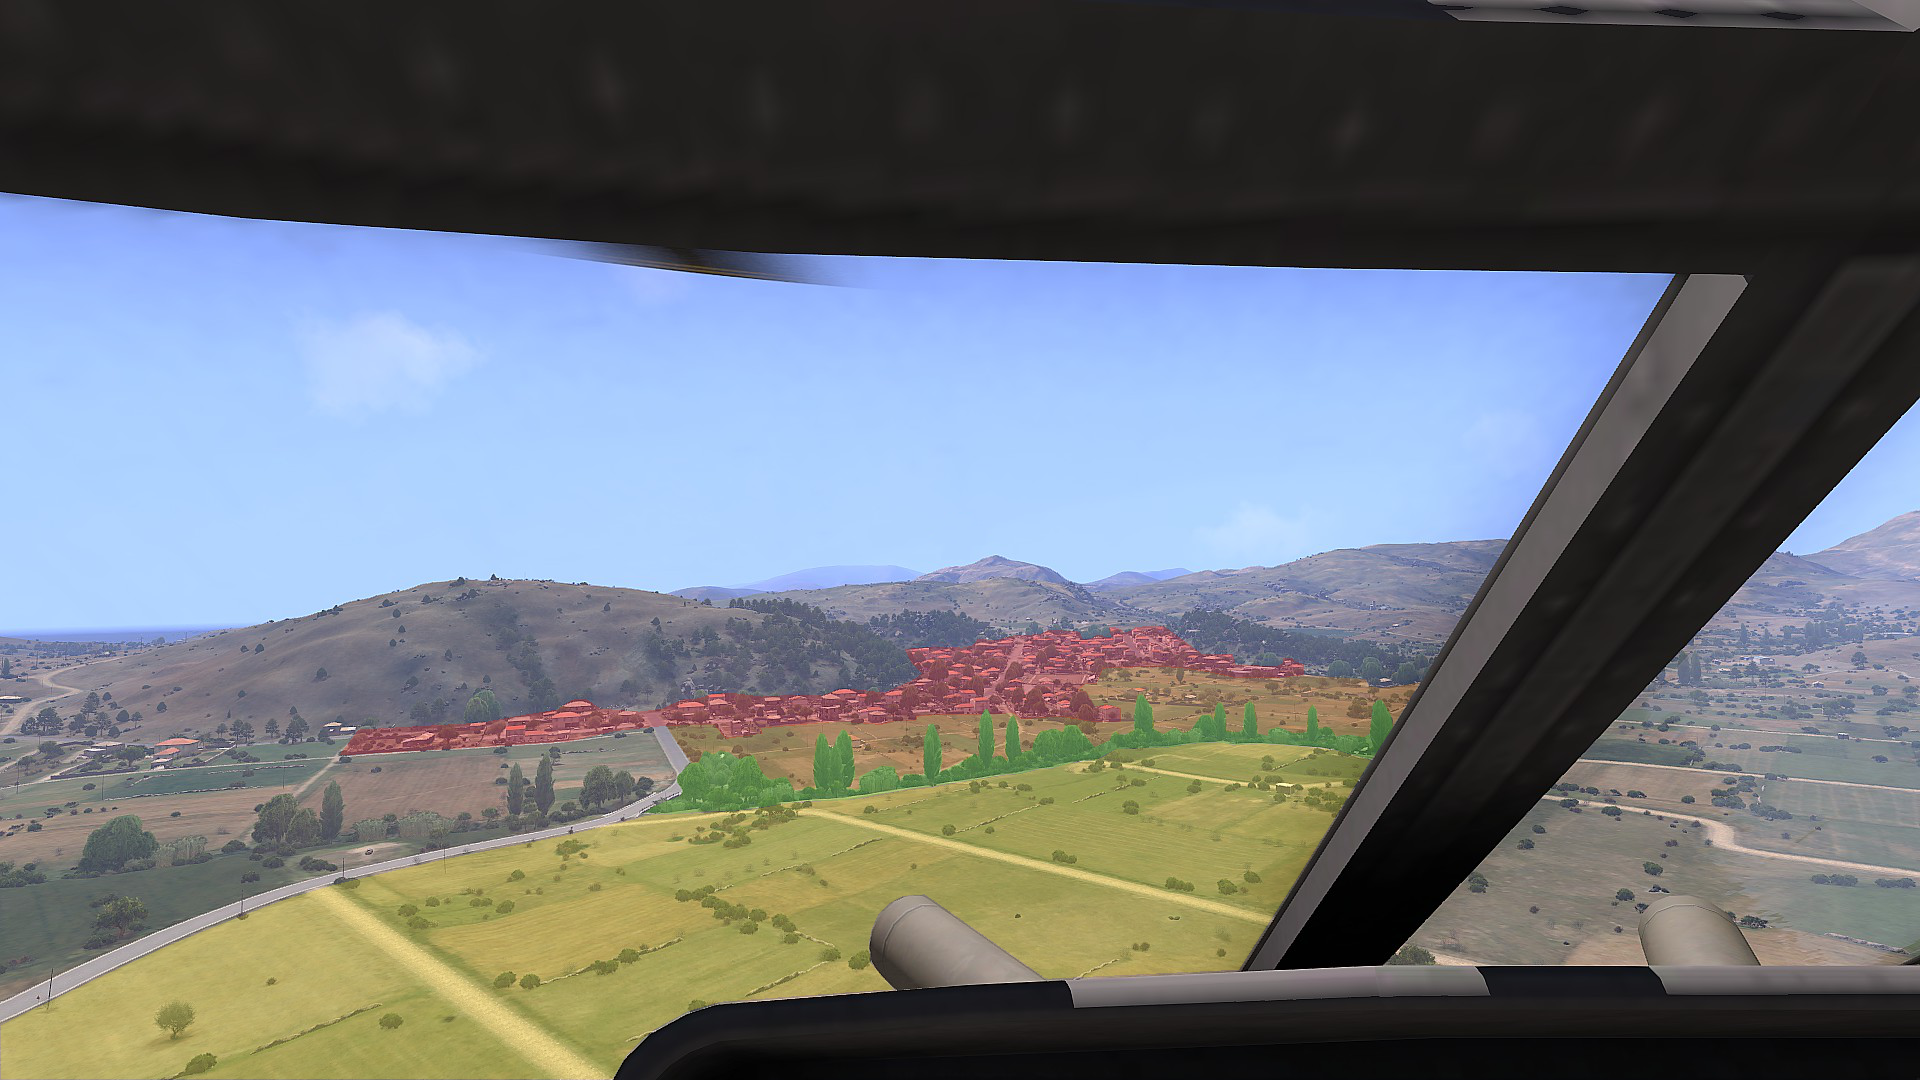
\includegraphics[width=0.95\linewidth]{../img/advanced/hubschrauber_+_infanterie/sicht-pilot}
	\end{figure}

\subsection{Lift-off}
	Sobald alle Aufgaben abgeschlossen sind oder der FAC die vollständige Anwesenheit durchgibt, führt der Pilot den Lift-off durch. In diesem Moment erlischt die Verantwortung vom FAC. 

\subsection{Worst Case Szenarios}
	Falls während dem Flug die Maschine beschädigt wird, werden alle Pläne und Aufträge verworfen. In diesem Moment ist oberste Priorität die Maschine unversehrt zu landen. In dem Fall, dass ein Helikopter bei einer Landung beschädigt wird, sind die nötigen Maßnahmen zu veranlassen den Helikopter wieder Instand zu setzen.
\pagebreak
\section{Verhalten bei Feindkontakt}
Wird ein Feind ausgemacht, so meldet ein Truppmitglied diesen an den TF.\\

Dies könnte im Truppfunk so gemeldet werden:\\
>>1 hier 6, Kontakt, stationäres MG auf 290°, Entfernung ca. 800\,m, Kalt<<

Eine andere Situation ergibt sich wenn der Feind das Feuer auf die eigene Stellung eröffnet. Hier hängt es von der Ausgabe des Feuerstatus ab. Ist Feuerstatus rot ausgegeben wird das Feuer nur erwidert wenn es ums blanke überleben geht.\\

Hier kommen die Kommandos >>Stellung wechseln<<, >>Feuer Frei<<, >>Ausweichen<< oder >>Verzögern und Ausweichen<< in Frage.\footnote{Ausführlich in >>\nameref{sec:kommando}<< beschrieben}\\

In allen fällen gibt der TF das Kommando aus, wie sich verhalten werden soll.
\pagebreak
\chapter{Sanitätssystem}
\pagebreak
\chapter{Konvoi}
	Wenn das Einsatzgebiet in weiter Ferne liegt, eine Verlegung mit einem Helikopter nicht möglich ist und die Wanderschuhe durchgelaufen sind, greift man auf seinen Fuhrpark zurück. Damit die Verlegung aber nicht in einer Offroad-Rally endet, befassen wir uns mit dem Konvoi und der Einbindung von Fahrzeugen außerhalb der Panzerwaffe in den infanteristischen Kampf. 

\subsection{Vorbereitungen für den Konvoi}
	Die Vorbereitung des Konvois umfasst mehrere Teilbereiche: Die Karten- und Routenarbeit, die Reihenfolge der Trupps innerhalb des Konvois, das Aufsitzen der Trupps auf die Fahrzeuge und das Herstellen der Konvoi-Formation.

\subsubsection{Karten- und Routenarbeit für den Konvoi}
	Die Kartenarbeit wird im TTT von der Zugführung (Trp. Grün)  übernommen. Trp. Grün bildet hierbei gleichzeitig das Führungsfahrzeug im Konvoi - Nicht zu verwechseln mit dem Fahrzeug, das an der Spitze den Konvoi anführt! \\
	Die Zugführung plant die Route nach verschiedenen Gesichtspunkten und richtet dafür Checkpoints (CP's) ein, die der Konvoi während der Fahrt zu passieren hat: 

	\begin{itemize}
		\item schnellstmögliche Annäherung an das Zielgebiet
		\item möglichst sichere Route für den Konvoi
		\item Ausnutzung von Gelände und Tageszeit zu unserem Vorteil
		\item CP's sind dabei so zu setzen, dass sie markante Objekte sind, die man schnell im Gelände ausmachen kann (Kirchen, Tankstellen etc.) und/oder die Möglichkeit zum Sammeln des Konvois bieten und/oder eine dem Gelände entsprechend gute Position für eine Overwatch ermöglichen und/oder einen Richtungswechsel des Konvois markieren (Kreuzungen)
		\item CP's sind nicht mit Haltepunkten gleichzusetzen! Wenn an einem CP gehalten werden soll wird das von der Zugführung befohlen!
	\end{itemize}

\subsubsection{Die Reihenfolge der Trupps im Konvoi}
	Die Zugführung passt die Reihenfolge der Trupps den Gegebenheiten und der Verfügbarkeit anderer motorisierter Elemente an.

\subsubsection{Das Aufsitzen auf Fahrzeugen}
	Gerüchteweise werden immer wieder Kameraden im Konvoi vergessen oder 30 Mann warten, bis der vermeintlich Abtrünnige (der schon im Fahrzeug sitzt) endlich einsteigt. \\
	Bestiegen werden Fahrzeuge in folgender Reihenfolge – von der höchsten Zahl zur niedrigsten (Truppführer). Dabei wird vor dem Einsteigen per Funk mitgeteilt, dass man einsteigt (>>6 steigt ein!<<, >>5 steigt ein!<< usw.). \\
	Der übliche Befehl eines Truppführers lautet hierbei >>Trupp XYZ, in umgekehrter Reihenfolge aufsitzen!<<.
Im Fahrzeug wird durchgezählt – der Truppführer beginnt. Nach Durchzählung gibt der Truppführer der Konvoi-Führung durch, dass der Trupp aufgesessen und bereit ist. \\
	Beim Absitzen steigt wiederum die höchste Zahl als Erstes aus – die niedrigste Zahl zuletzt (Truppführer). Somit kann der Truppführer davon ausgehen, dass tatsächlich sein gesamter Trupp abgesessen ist. Auch hier gibt man kurz durch, dass man absitzt (>>6 raus!<<, >>5 raus!<< usw.). \\

\subsubsection{Besetzung der Positionen im Fahrzeug}
	Führen, fahren, funken, funzt? \\
	Nein, tut es nicht! \\
	Deswegen fährt im TTT immer die größte Nummer, im Normalfall also Nummer 6. Truppführer, Funker und Medics haben striktes  Fahrverbot, sie haben andere Aufgaben (>>So, ich näh den jetzt hier mal fix zu …- Schau auf die Straße Grunt, schau auf die Stra...<< *BUMM*). \\
	Bei einem bewaffneten Fahrzeug wird die Position des Schützen im Normalfall von der Nummer 5 übernommen. Somit haben wir das Fahrzeug unter der Kontrolle eines Buddyteams, die anderen beiden Buddyteams werden nicht auseinander gerissen und sind voll einsatzfähig. Des Weiteren stellen wir so auch eine Feuerüberlegenheit her, denn die Nummern 3 und 4 bilden das MG-Team. Somit stehen dem Truppführer 2 Schwerpunktwaffen zu Verfügung (MG-Team + Fahrzeugwaffe). \\
	Der Truppführer nimmt hierbei die Position des Beifahrers ein, er hat ein GPS und kann den Fahrer einweisen. \\
	Idealerweise sieht also ein besetztes Fahrzeug im TTT wie folgt aus:

	\begin{itemize}
		\item Nummer 1 (Trp.Fhr.) - Beifahrer
		\item Nummer 2 (Grenadier) - Passagier
		\item Nummer 3 (MG-Assi) - Passagier
		\item Nummer 4 (MG) - Passagier
		\item Nummer 5 (AT/AA-Schütze) - Fahrzeugwaffenschütze
		\item Nummer 6 (AT/AA-Schütze) - Fahrer
	\end{itemize}

\subsubsection{Formation des Konvois}
	Wir fahren zwei unterschiedliche Konvoi-Formen:
	\begin{itemize}
		\item Offener Konvoi: Kolonne, Abstand von maximal 100 Metern (taugt für flaches Gelände, Wüsten, gute Wetterlage, guter Straßenbelag), hohe Geschwindigkeit.
		\item Geschlossener Konvoi: Kolonne, Abstand von unter 25-50 Metern (taugt für urbane Umgebung, schlecht einsehbares Gelände (Hügel, Bewuchs) hohes Verkehrsaufkommen, schlechte Wetterlage, schlechter Untergrund), niedrige Geschwindigkeit
	\end{itemize}

	ARMA-Reality-Check: Bei vielen Desyncs empfiehlt es sich einen höheren Abstand zwischen die Fahrzeuge zu legen. Auch mehr als 100 Meter. \\
	Generell sind die Abstände des Konvois der Topographie, der Sichtverhältnisse und der Feindlage anzupassen. Ein Auffahren auf unter 5 Meter (oder eine Fahrzeuglänge) ist unter allen Umständen zu vermeiden, außer explizit angeordnet. \\
	Dazu folgende Faustregeln:

	\begin{itemize}
		\item Je offener und höher die Sichtweite, umso größer kann der Abstand zwischen den Konvoi-Fahrzeugen gewählt werden. Trotzdem MUSS im Konvoi in der Regel Sichtkontakt zum vorderen Fahrzeug immer möglich sein.
		\item Je unübersichtlicher das Gelände, desto enger wird der Konvoi gefahren. Auch bei hohem Verkehrsaufkommen (zivile Fahrzeuge auf der Fahrbahn) wird eine eher enge Fahrweise bevorzugt.
	\end{itemize}

Vor- und Nachteile von dem offenen und geschlossenen Konvoi \\
	Generell ist eine lockere Formation in Takistan bevorzugen, da es sich meist um offenes Gebiet handelt. Die lockere Formation sorgt dafür, dass der Gegner nicht den gesamten Konvoi gleichzeitig unter Feuer nehmen kann und das IEDs nicht mehrere Fahrzeuge ansprengen können. Zudem ermöglicht der größere Abstand zwischen den Fahrzeugen mehr Manöverwege (Flanken, Ausweichen) und bessere Reaktion auf Gefahren. Nicht zuletzt reduziert es die Gefahr von Auffahrunfällen drastisch.  \\
	Die geschlossene Formation ist im Personenschutz und beim Transport von High Value Gütern bevorzugt, da die enge Formation verhindert, dass sich etwas >>zwischen<< den Konvoi setzen kann – und Feuerkraft auf einen sehr engen Raum zusammenfasst. Gleichzeitig ist die enge Formation deutlich schwieriger zu fahren (Auffahrunfälle) und erfordert vorausschauendes Fahren und ein eingespieltes Team. \\

\subsubsection{Struktur eines Konvois}
	Der Konvoi ist so strukturiert, dass er maximale Sicherung bietet. Dabei unterscheiden wir zwischen: \\
	Einem >>Dreier Konvoi<<(3 Elemente) und einem >>Fünfer Konvoi<< (5 Elemente).Egal wie groß die Mannschaft – ein Konvoi ist immer in mind. 3 Teile zu unterteilen – optimalerweise aber in fünf.  \\
Der >>Dreier Konvoi<<

	\begin{itemize}
		\item 1ste Sicherungselement
		\item Transport und Führung
		\item 2tes Sicherungselement
	\end{itemize}

	Die  Advanced Guard sorgt für die Sicherheit nach vorne und klärt die zu befahrende Wegstrecke auf. Die Transportgüter und die Führung befinden sich in dem mittleren Teil des Konvois und sichern die Seitenbereiche rechts und links ab. Die Nachhut sorgt für die rückwärtige Sicherung und gilt als schnelle Einsatztruppe bei Feuerüberfällen. \\
Der >>Fünfer Konvoi<<
Eine verbesserte Variante des Konvois im TTT besteht aus 5 Elementen:

	\begin{itemize}
		\item Recon (advance guard/Vorhut)
		\item 1tes Sicherungselement
		\item Transport und Führung
		\item 2tes Sicherungselement
		\item Nachhut (rear guard)
	\end{itemize}

	Durch diese Struktur übernehmen das 1ste und das 2te Sicherungselement die Seitenabsicherung und bei Bedarf ebenfalls die Sicherung nach vorne und hinten. Das Recon-Element kann den Abstand zum Konvoi vergrößern und wird als variables Aufklärungselement eingesetzt. Gefahren werden so frühzeitiger erkannt. Die Nachhut kann ebenfalls den Abstand vergrößern und so bei jedem Halt als Overwatch-Element dienen - sowie als Reserve-Einheit an Brennpunkte gezogen werden. \\

\subsection{Die Fahrt}
\subsubsection{Geschwindigkeit eines Konvois}
	Die Geschwindigkeit sollte in etwa 50-70 \% der Maximalgeschwindigkeit des LANGSAMSTEN Fahrzeuges im Konvoi sein. Jedes Fahrzeug braucht eine Beschleunigungsreserve für den Notfall und für das Regulieren des Abstandes. Das Fahren mit Höchstgeschwindigkeit ist nur im Notfall erlaubt und nur über kurze Strecken. \\
	Tipp: ARMA bietet 3 Standardgeschwindigkeiten für Fahrzeuge (tatsächliche ist Geschwindigkeit abhängig vom Fahrzeugmodell und Untergrund) \\

	\begin{itemize}
		\item Langsam: [Strg] + [W]
		\item Normal: [W]
		\item Schnell:[Shift] + [W]
	\end{itemize}

\subsubsection{Halten eines Konvois}
	Im TTT gibt es zwei relevanten Halteformationen für Konvois

	\begin{itemize}
		\item Halt in Kolonnenformation (-----)
		\item Halt in Fischgrätenformation (o<<<<)
	\end{itemize}

	Wichtig: Halten ist KEIN Parken. Halten bedeutet, dass jederzeit und sofort die Fahrt aufgenommen werden kann. Also keine >>für kleine Tiger<< für Fahrer während eines Haltes. \\
	Der Halt in Kolonnenformation wird auf der Straße vollzogen und die Fahrformation und Ordnung wird beibehalten. Zum Halt wird dabei an den Straßenrand gefahren (in der Regel rechts), um einen Rettungskorridor freizuhalten. \\
	Der Halt in Fischgrätenformation ist eine defensivere Formation als die Kolonnenformation und ermöglicht eine bessere Absicherung. Dabei wird das Fahrzeug von der Straße seitlich (rechts und links abwechselnd) im freien Gelände und in einem Winkel von etwa 45 Grad  zur Straße positioniert. Bei kurzem Halt, Abstand zur Straße etwa 5-10 Meter – und von Fahrzeug zu Fahrzeug in etwa 20-50 Meter. Bei längeren Halt wird die Sicherungselemente 100 Meter ins freie Feld gefahren und der Konvoi von dort aus gesichert. Würde man von oben auf den Konvoi sehen, entstünde die Form einer Fischgräte. \\
	Wann wird welche Formation angewendet? \\
	Die Fischgrätenformation ist die bessere, weil sicherere Formation. Allerdings erfordert sie deutlich mehr Platz, ein freies Feld rechts und links und gut zu befahrenden Untergrund. Wird auf ein schnelles Weiterfahren besonderen Wert gelegt oder es nicht möglich ist, die Straße zu verlassen (Mauern, Hindernisse, Brücke, abschüssiges Gelände) wird in Kolonnenformation gehalten. \\
\subsubsection{Sicherungsbereich in Fahrt}
Sicherungsbereiche während der Fahrt in 3er Formation

	\begin{itemize}
		\item Recon (advance guard) Sicherungsschwerpunkt nach vorne
		\item Transport und Führung – Sicherungsschwerpunkt nach rechts und links
		\item Nachhut (rear guard) - Sicherungsschwerpunkt nach hinten
	\end{itemize}

Sicherungsbereiche während der Fahrt in 5er Formation

	\begin{itemize}
		\item Recon (advance guard) Sicherungsschwerpunkt nach vorne
		\item 1tes Sicherungselement Sicherungsschwerpunkt nach rechts und links
		\item Transport und Führung  
		\item 2tes Sicherungselement Sicherungsschwerpunkt nach rechts und links
		\item Nachhut (rear guard) - Sicherungsschwerpunkt nach hinten
	\end{itemize}

\subsubsection{Sicherungsbereich in Fahrt – Personal}
	Während der Fahrt in einem bewaffneten Fahrzeug (HMMWV, MRAP, Fennek, Puma) gibt es in der Regel 3 Positionen zu besetzen.

	\begin{itemize}
		\item Fahrer (größte Nummer)
		\item Beifahrer/Kommandant (Truppführer) -> Wird entschieden
		\item Schütze (zweitgrößte Nummer)
	\end{itemize}

	In einem Fahrzeug mit Kommandantenposten (Fennek, MRAP Puma, etc.) wird die Wärmebild vom Truppführer besetzt, der Funker sitzt auf den Beifahrersitz vorne (Fennek, MRAP) und blickt nach vorne und rechts. \\
	In einem Fahrzeug OHNE Kommandantenposten (HMMWV, Toyota, LKW), wechselt der Truppführer auf den Beifahrersitz vorne. Der Truppführer hat die Aufgabe, den Sicherungsbereich vorne und rechts im Auge zu behalten. \\
	Bei Bewaffneten Fahrzeugen teilen sich die Fahrzeuge die Sicherungsbereiche nach Schwerpunkten auf. Das heißt, die Bordkanone wird auf den Schwerpunkt ausgerichtet. Dabei gilt der Merksatz >>rechts vor links<< – illustriert an folgendem Beispiel: 

	\begin{itemize}
		\item Fahrzeug 1 – Recon – Sicherung Schwerpunkt vorne
		\item Fahrzeug 2 – Sicherungselement 1 – Sicherungsschwerpunkt rechts
		\item Truppführung – Fahrzeug unbewaffnet
		\item Fahrzeug 4 – Sicherungselement 2 – Schwerpunkt links
		\item Fahrzeug 5 – Nachhut – Sicherung Schwerpunkt hinten
	\end{itemize}

	Bei Fahrzeugen mit Bewaffnung und Kommandantenposten ist darauf zu achten, dass beide unterschiedliche „Uhrzeiten“ überwachen. \\
	zweites Beispiel:

	\begin{itemize}
		\item Fahrzeug 1 – Recon – Sicherung Schwerpunkt vorne
		\item Fahrzeug 2 – Sicherungselement 1 – Sicherungsschwerpunkt rechts
		\item Fahrzeug 3 – Sicherungselement 1 – Sicherungsschwerpunkt links
		\item Fahrzeug 4 – Sicherungselement 1 – Sicherungsschwerpunkt rechts
		\item Fahrzeug 5 – Truppführung – Fahrzeug unbewaffnet
		\item Fahrzeug 6 – Sicherungselement 2 – Schwerpunkt links
		\item Fahrzeug 7 – Sicherungselement 2 – Sicherungsschwerpunkt rechts
		\item Fahrzeug 8 – Nachhut – Sicherung Schwerpunkt hinten
	\end{itemize}

\subsubsection{Sicherungsbereich im Halt}
	Hier muss klar unterschieden werden, zwischen den Methoden im  realen Leben und den Methoden in ARMA. Der Grund: Das Schadensmodell der Fahrzeuge in ARMA 3 ist (wie in allen Teilen zuvor) äußerst mangelhaft. Die Fahrzeuge tendieren ohne Vorwarndung in einen Feuerball aufzugehen. \\
	Was wieder nicht ganz so unrealistisch ist: Der Gegner (in diesem Falle die KI) kämpft mit Panzerbrechende Munition besonders erfolgreich Fahrzeuge - meist deutlich früher, als die AT-Schützen aufgeklärt wurden. Dies führt häufig dazu, dass bei >>realistischer<< Verhaltensweise der komplette Trupp im Feuerball stirbt. Daher gibt es, abweichend von den üblichen Doktrinen, Abweichungen im TTT 

	\begin{itemize}
		\item Es ist absolut zu vermeiden, die Fahrzeuge als Deckung zu verwenden. Das gilt sowohl für Softskin (leichte Fahrzeuge, nicht beschusssicher) als auch für Hardskin (gepanzerte Fahrzeuge)
		\item Die Sicherung von Fahrzeugen oder dem Konvoi findet IMMER in Deckung und IMMER etwa 15 Meter vom Fahrzeug entfernt statt - Ausnahme - das Fahrzeug ist nicht besetzt.
		\item Es kommt häufig vor, dass ein Trupp- oder Zugführer das komplette aussteigen anordnet, auch der Schütze und Fahrer. Das hängt damit zusammen, dass leere Fahrzeuge nicht angegriffen werden. Stattdessen werden ERST die Feinde aufgeklärt und dann bei Bedarf das Geschütz bemannt - wir verwenden also das Fahrzeug häufig als >>Joker<<  der erst gezogen wird, wenn wir das Gefährt sicher einsetzen können.
	\end{itemize}

Beim Halt gibt es zwei Arten des Absitzen - die Befehle:

	\begin{itemize}
		\item Absitzen (Alle steigen aus bis auf den Schützen - der Fahrer bleibt außen AM Fahrzeug in Rufweite zum Schützen - 5-10 Meter). Damit er sofort einsteigen kann.
		\item Verlassen (alle verlassen das Fahrzeug und lassen es stehen - der Trupp bewegt sich mind. 15 Meter vom Fahrzeug weg
	\end{itemize}

	Sicherungsrichtung beim Halt \\
Egal ob Kolonnenformation oder Fischgrätenformation: Im Konvoi bauen wir die Sicherung auf die Seite auf, die in unserem Verantwortungsbereich lag (bei der Fahrt). Also entweder Rechts oder Links. Dabei (wichtig!) entfernen wir uns von den Fahrzeugen und suchen eigenständig Deckung. Bei kleineren Konvois (3er Konvois) tragt der Mittelteil die Verantwortung für die seitliche Absicherung. Beim 3er Konvoi unbedingt zu vermeiden ist eine Absicherung, in der in der Mitte das Fahrzeug die Sicht auf den eigenen Trupp verhindert - und den Trupp in zwei Teile aufteilt. Besser ist es, sich vom Fahrzeug weg zu bewegen und an erhöhter Position in Deckung eine 360 Grad-Sicherung aufzubauen, mit Überblick auf den Konvoi. \\
	Die Recon richtet ihren Sicherungsbereich nach vorne aus. Das bewaffnete Fahrzeug ist nach Möglichkeit teilverdeckt nahe der Straße abzustellen - Aber NICHT auf Straßenkreuzungen oder ähnliches. \\
	Die Nachhut stoppt in Overwatchposition - dabei bleibt in der Regel das schwere MG besetzt, während ein Teiltrupp den Rückraum sichert. \\

\subsubsection{Konvoifunk und Kommunikation}
	VOR der Konvoi-Bildung wird vom Fahrer (!) und Truppführer (!) sich auf einen zusätzlichen Funkkanal eingewählt. Der Standard-Konvoi-Kanal im TTT ist 99 auf der Shortrange. Funker bleibt auf seinen Frequenzen. Nur Trupp- und Zugführer und OPL sprechen auf dem Kanal. Fahrer empfängt nur. Bei Ausfall vom Truppführer übernimmt Funker die Position vom TF. \\
	Über den Konvoikanal werden durchgegeben:

	\begin{itemize}
		\item Bewegung und Halt 
		\item Bedrohungslagen
	\end{itemize}

	Beispiel für einen Funkspruch bei plötzlichen Kontakt: Break, Break, Vorhut 1, heißer Kontakt, 3 Uhr. \\
	Alles andere läuft über die üblichen Kanäle. \\

\subsection{Reaktion auf verschiedene Bedrohungslagen}
in Arbeit
Battledrill: Durchstoßen
Kommt noch…
Battledrill: Bekämpfen
Kommt noch…
Battledrill: Ausweichen


\pagebreak
\chapter{Kartenarbeit}
\subsection{Umgang mit dem Kompass}
Generelle Feindsichtungen nach R-E-Z (Richtung-Entfernung-Ziel) Prinzip \\

Gut geeignet für schnelle Ausrichtung im Gelände. Simple Information über mögliche Kontakte, besonders wenn man verteilt steht.
\begin{figure}[!h]
	\centering
	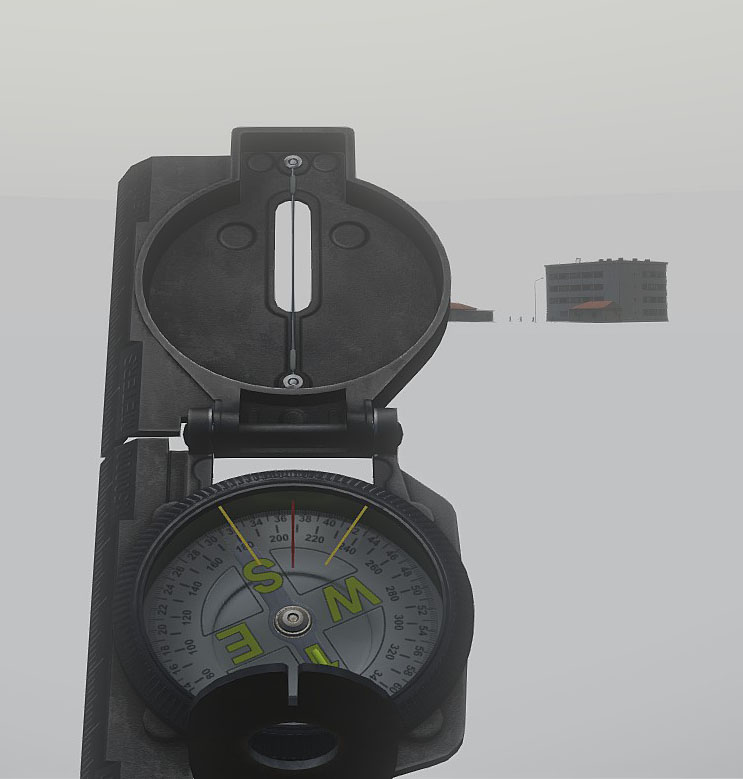
\includegraphics[width=0.7\textwidth]{../img/advanced/kartenarbeit/Kompass1}
	\caption{Beispiel: Sichtung 4er Infanterie Patrouille in Stadtgebiet}
\end{figure}\\
	
Für Zieleinweisung
\begin{itemize}
	\item Ziel mit Feldstecher lokalisieren, mit dem Fadenkreuz anpeilen.
	\item Ohne sich zu bewegen auf den Kompass Wechseln für die genaue Gradzahl bzw. Ausrichtung des Kompassdrahts an markanten Stellen oder auf den Feind, sofern Sichtbar.
\end{itemize}

\begin{figure}[!h]
	\centering
	\includegraphics[width=0.75\textwidth]{../img/advanced/kartenarbeit/kompass2}
\end{figure}

Angabe: >>Kontakt im Südwesten 300 m, links vom hohen Bürogebäude, 4 Mann Patroullie, kalt<< (Bitte beachten das weitere Informationen hilfreich sein können z.B. Art der Bewaffnung)\\

Feindsichtungen nach Gradzahlen
Gut geeignet für eindeutige Bestimmung von Feinden für Gruppenscharfschützen und Fahrzeuge, die entweder dicht bei euch stehen oder in einer Linie hinter mit eurer Position stehen. Auch sehr nützlich für die präzisere Kartenmarkierung von Feinden.
\begin{figure}[!h]
	\centering
	\includegraphics[width=0.75\textwidth]{../img/advanced/kartenarbeit/kompass3}
	\caption{Situation: Einzelner feindlicher Kontakt auf HQ Gebäude}
\end{figure}\\

Für Zieleinweisung
\begin{itemize}
	\item Ziel mit Feldstecher lokalisieren, mit dem Fadenkreuz anpeilen.
	\item Ohne sich zu bewegen auf den Kompass Wechseln für die genaue Gradzahl bzw. Ausrichtung des Kompassdrahts an markanten Stellen oder auf den Feind, sofern Sichtbar.
\end{itemize}

\begin{figure}[!h]
	\centering
	\includegraphics[width=0.65\textwidth]{../img/advanced/kartenarbeit/kompass4}
\end{figure}
Angabe: >>Kontakt NW, 319° von meiner Position, 500m, einzelner Schütze auf dem Militärgebäude, kalt.<<\\

Feindsichtungen mit MILS (Strich / Artilleriepromille) \\

Hierbei werden die natürlichen Gradzahlen in einem Volkreis mit 6400 Einheiten aufgeteilt, was die Zieleinweisung bei über 1000m einen Seitenabstand des Ziels von einem Meter ergibt. Diese befinden sich auf dem 3., äusseren Zahlenring des Kompasses.\\
Gut geeignet bei sehr weiten Entfernungen 900m+, wo der Winkel der Gradzahlen sehr stark zusammenläuft um sehr exakte Anweisungen für Scharfschützen zu geben bzw. für Mörser / Artillerie Einweisung. Geht nicht ohne dass man direkt nebeneinander steht oder dies entsprechend der Position der Artillerie umrechnet.  \\

\begin{figure}[!h]
	\centering
	\includegraphics[width=0.75\textwidth]{../img/advanced/kartenarbeit/kompass5}
\end{figure}
Situation 2 Infanterieposten auf einem HQ Gebäude. Nur der Rechte soll von unserem Scharfschützen ausgeschaltet werden.\\
\begin{itemize}
 	\item Mit Feldstecher anvisieren.
	\item Ohne sich zu bewegen den Kompass rausholen und im äussersten Zahlenringen ablesen (Gradzahl ist bei rechtem oder linken Pfosten beides 320°) . Hierfür sollte man exakt hinter oder direkt neben dem Schützen positioniert sein.
	\end{itemize}
\begin{figure}[!h]
	\centering
	\includegraphics[width=0.65\textwidth]{../img/advanced/kartenarbeit/kompass6}
	\caption{>>Kontakt auf 320° meiner Position, 900 m, Strich 5690 , einzelner Schütze, kalt<<}
\end{figure}

\pagebreak
\subsection{Umgang mit der Karte}

	Navigation mit der Karte \\

	Die in Arma 3 verwendete topographische Karte ist sehr nützlich um geeignete Landezonen, Overwatchpositionen, Deckungsmöglichkeiten und Antrittswege im Voraus zu erkennen. Wichtig ist, dass hierbei die Höhenlinien und Symbole auf der Karte richtig interpretiert werden. Je enger die Höhenlinien, desto Steiler das Gelände. \\

	Hier als Beispiel von einem relativ schmalen Tal, das nach Norden, Westen und Süden von Bergen umgeben ist. \\
\begin{minipage}[t]{1\textwidth}
	\centering
	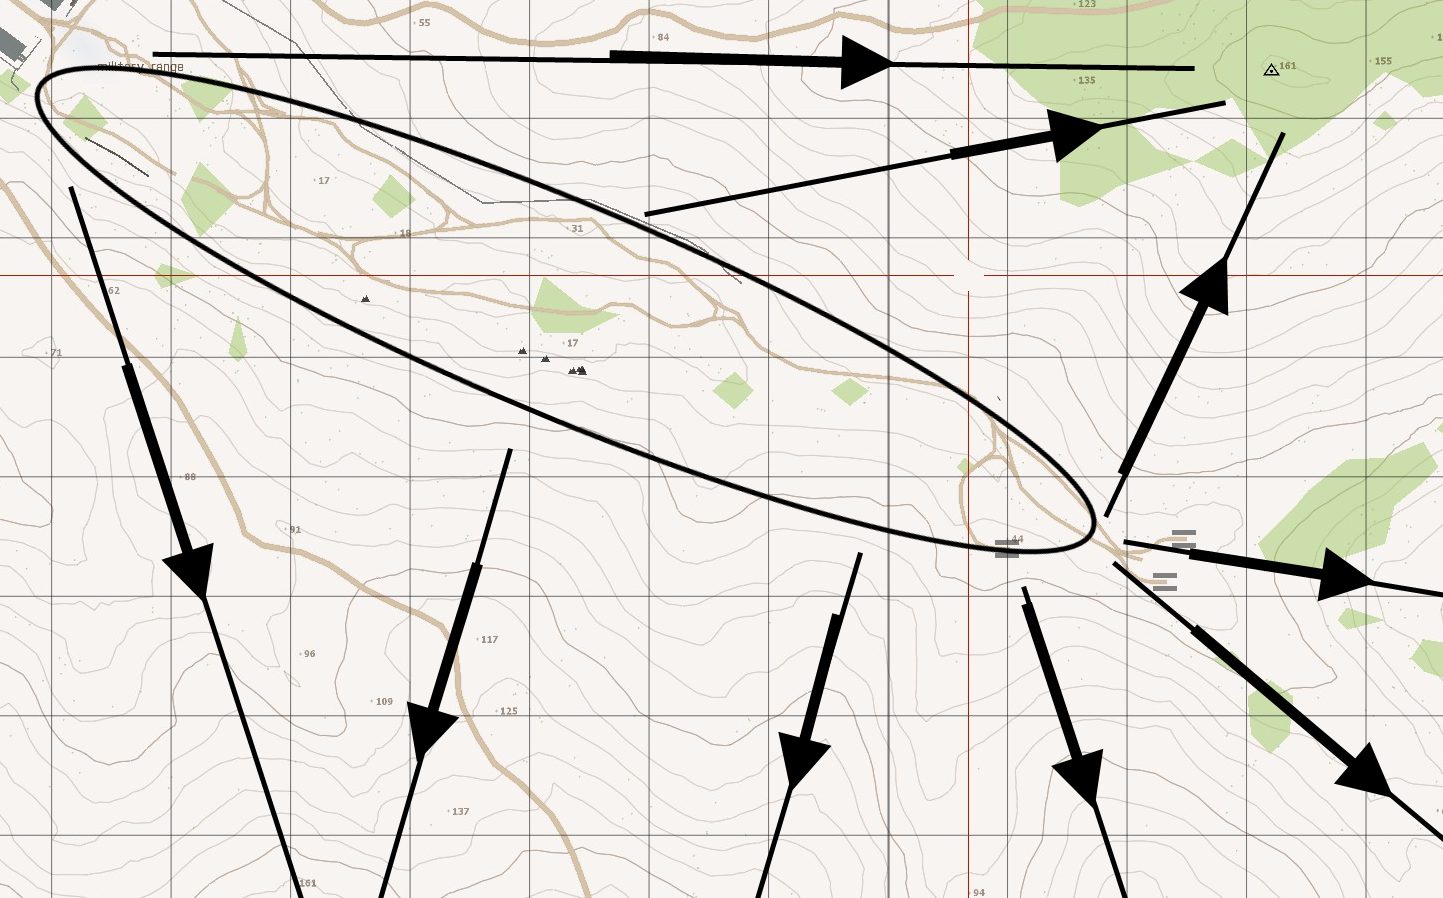
\includegraphics[width=\textwidth]{../img/advanced/kartenarbeit/Karte1.png}
\end{minipage}

	Markante Linien sind, je nach Zoomstufe im Abstand von 1 bis 25m zueinander, beginnend mit der Wasserlinie 0 m. Berggipfel werden mit einem Dreieck mit Punkt in der Mitte dargestellt, andere Hügel mit Zahlen (Meterangabe). Oft nutzt man diese auch zur Kommunkation >>Hill 68<< ist dann zB. der 68 m Hohe Hügel im entsprechenden Planquadrat. \\

\begin{minipage}[t]{1\textwidth}
	\centering
	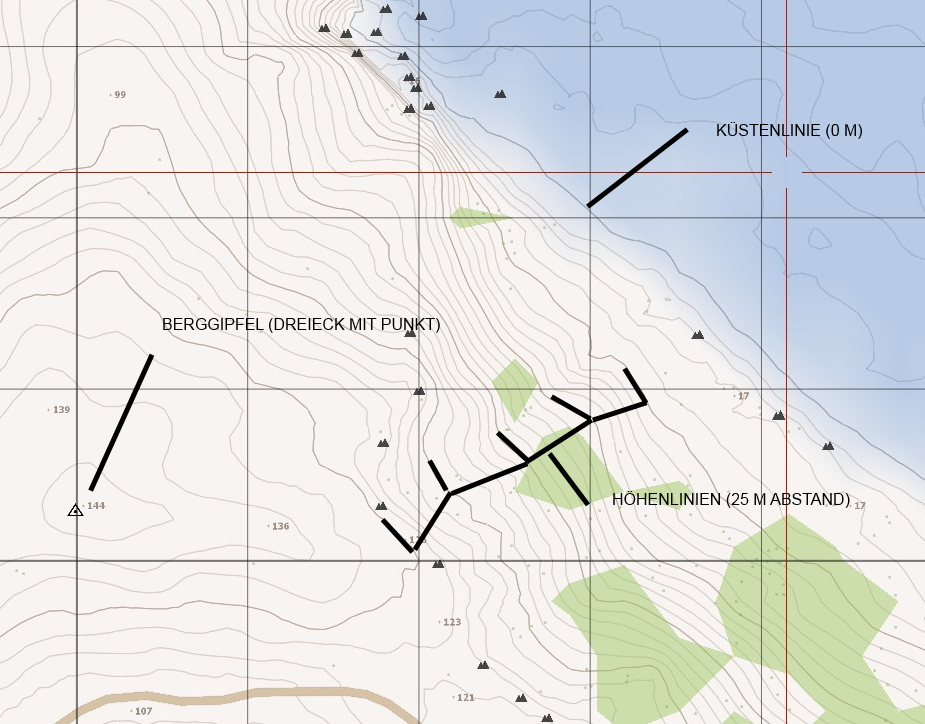
\includegraphics[width=\textwidth]{../img/advanced/kartenarbeit/Karte2.png}
\end{minipage}

	Kartenkoordinaten werden in der Kartenansicht immer unter eurem Cursor angezeigt. Falls euch welche gegeben werden, kann dies auf zwei Wege erfolgen: „Position xxx-yyy“ oder „Planquadrat xx-yy“. Die erste Zahlenfolge bezeichnet immer die Koordinatenspalten und die zweite Zahlenfolge die Koordinatenreihen. X ist die obere, horizontale Achse, Y ist die linke, senkrechte Achse. \\

	Die Karte selbst lässt sich fliessend per Mausrad Zoomen, die Gitternetzlinien sind in der weitesten Zoomstufe in 1km Abständen, sobald man näher heranzoomt ändern sich diese zu 100 m Abständen. So lassen sich auch Feindpositionen bzw. Distanzen zu diesen besser abschätzen. \\

	Die diagonale Distanz der 100 m Kästchen sind ca. 140 m. \\

\begin{minipage}[t]{1\textwidth}
	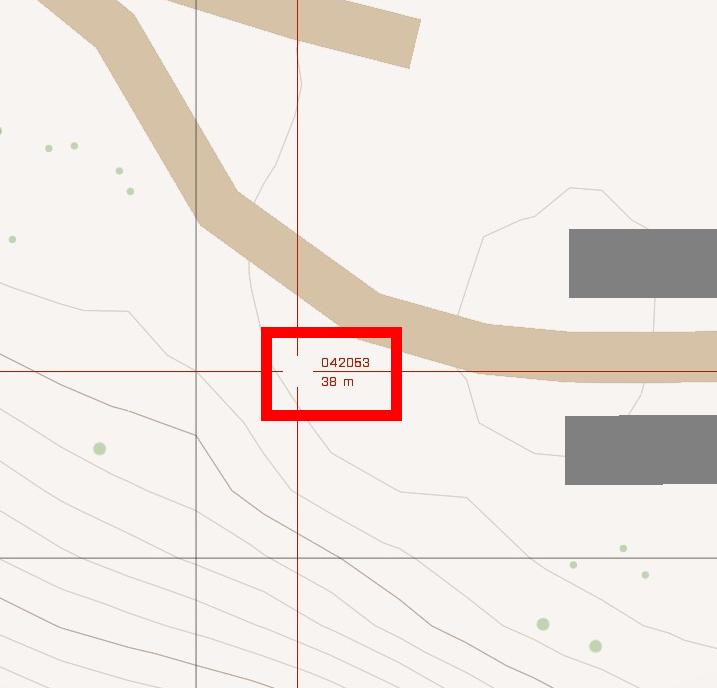
\includegraphics[width=\textwidth]{../img/advanced/kartenarbeit/Karte3.png}
\end{minipage}

	Diese Koordinaten werden auch auf eurem GPS oben links angezeigt, so lässt sich eure Position immer genau bestimmen, falls verlangt wird, dass ihr eure eigene Position markiert bzw. um festzulegen wo Feinde zu markieren sind. \\

\begin{minipage}[t]{1\textwidth}
	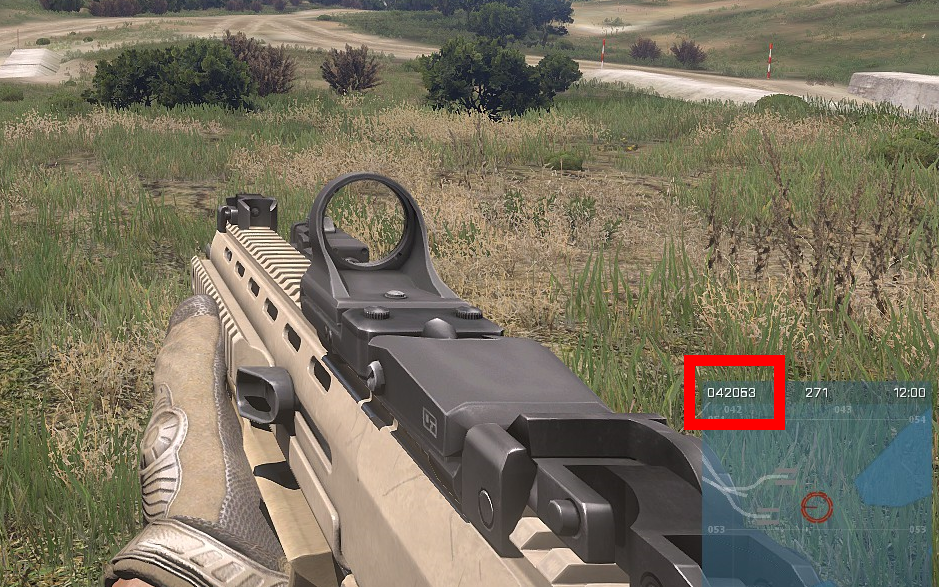
\includegraphics[width=\textwidth]{../img/advanced/kartenarbeit/Karte4.png}
\end{minipage}
\input{./advanced/kartenarbeit/symbole}
\input{./advanced/kartenarbeit/feindeinheiten}
\input{./advanced/kartenarbeit/operationsbefehl}


%Mods
%\part{SGA \& Tutorials}
%\chapter{SGA}
%\chapter{Gepanzerte Fahrzeuge}
\section{Der Schützenpanzer}
	Ein Schützenpanzer ist ein leicht gepanzertes Fahrzeug, welches das Bindeglied zwischen leichten Transportfahrzeugen und schweren Panzern darstellt. Primär dient ein SPz zur Unterstützung von verbündeten Infanteriekräften sowohl im urbanen- als auch im offenen Gelände. Innerhalb des Schützenpanzers bilden speziell ausgebildete Infanteriekräfte die Nahsicherung des Fahrzeuges, welche in einem späteren Kapitel näher erläutert werden.\\
	
	In Arma 3 stehen viele verschiedene Modelle eines SPz zur Verfügung, diese unterscheiden sich in Dingen wie:
	\begin{itemize}
		\item Fassungsvermögen von Infanterie
		\item Bewaffnung
		\item Visierung
		\item Ketten- sowie Radpanzer
	\end{itemize}
	
	In der folgenden Übersicht werden verschiedene Modelle präsentiert und ihre jeweiligen Spezifikationen aufgelistet.

\subsection{Modfahrzeuge}
	\begin{longtable}{lc} 
		\toprule
		Bradley (Blufor) & \multirow{2}{*}{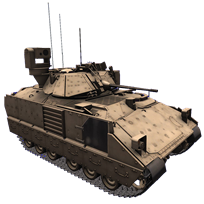
\includegraphics[width=0.4\textwidth]{./img/tutorials/spz/bradley}}\\
		\begin{minipage}[t]{0.4\textwidth}
			\begin{itemize}
				\item Platz für 9 Mann (3 Besatzung, 6 Infanteristen)
				\item Bewaffnung:
				\begin{itemize}
					\item 25 mm Bordkanone
					\item 7.62 mm koaxial MG
					\item TOW AT Raketen
				\end{itemize}
				\item Nebelmittelwurfanlage
				\item Kettenfahrzeug
			\end{itemize}
		\end{minipage}\\
		\midrule
		Puma (Blufor) & \multirow{2}{*}{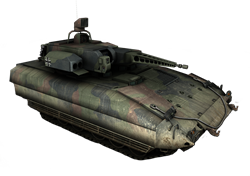
\includegraphics[width=0.4\textwidth]{./img/tutorials/spz/puma}}\\
		\begin{minipage}[t]{0.4\textwidth}
			\begin{itemize}
				\item Platz für 9 Mann (3 Besatzung, 6 Infanteristen)
				\item Bewaffnung:
				\begin{itemize}
					\item 30 mm Bordkanone
					\item 7.62 mm koaxial MG
					\item Spike AT Raketen
				\end{itemize}
				\item Nebelmittelwurfanlage
				\item Kettenfahrzeug
			\end{itemize}
		\end{minipage}\\	
		\bottomrule 
	\end{longtable}

\section{Bewaffnung und Panzerung von Schützenpanzer}
Schützenpanzer sind durch ihre modulare Bauweise in Sachen Bewaffnung und Panzerung äußerst flexibel aufrüstbar.

\subsection{Bewaffnung}
	Im Militär werden gegnerische Feindkräfte in Bezug auf Panzerung in drei Klassen unterteilt:
	\begin{longtable}{ll} 
		\toprule
		Typ & Definition\\
		\midrule
		Weich & Nicht gepanzerte Kräfte wie Infanterie, Transportfahrzeuge, etc.\\
		Halb-Hart & Leicht gepanzerte Ziele wie Schützenpanzer.\\
		Hart & Schwer gepanzerte Ziele wie Kampfpanzer.\\
		\bottomrule 
	\end{longtable}

	Standardmäßig ist ein Schützenpanzer mit einer Bordkanone, einem Maschinengewehr sowie einer Feuerleitanlage ausgestattet, welche eine effektive Bekämpfung feindlicher Panzerkräfte ermöglicht.
	\begin{longtable}{ll} 
		\toprule
		Waffensystem & Zieltyp\\
		\midrule
		\multirow{2}{*}{Bordkanone} & Weich\\
		& Halb-Hart\\
		Maschinengewehr (Koaxial) & Weich\\
		\multirow{2}{*}{Granatwerfer} & Weich\\
		& Halb-Hart\\
		\bottomrule 
	\end{longtable}

\subsection{Panzerung}
	Schützenpanzer bieten in der Realität eine meist gut ausgebaute Panzerung, welche so in ArmA jedoch nicht implementiert wurde. Folgende Punkte sollten im Kampfgeschehen beachtet werden.\\

	Ein SPz ist gegen Handfeuerwaffen nahezu vollständig geschützt, bietet gegen Beschuss von mobiler Panzerabwehr jedoch nur bedingt Schutz. Dies ist von der Position des Einschlags des Projektils sowie Entfernung abhängig.\\
	Beschuss durch feindliche, harte Kräfte enden meist in einem Totalverlust des Fahrzeuges, sodass eine Konfrontation mit diesen Kräften um jeden Preis vermieden werden sollte.\\

	Daher ist zu empfehlen, den Schützenpanzer nur als Unterstützungselement einzusetzen (siehe Bild) und durch verbündete, abgesessene Infanterie, im Nahbereich zu sichern.\\
	\begin{figure}[htbp]
		\centering
		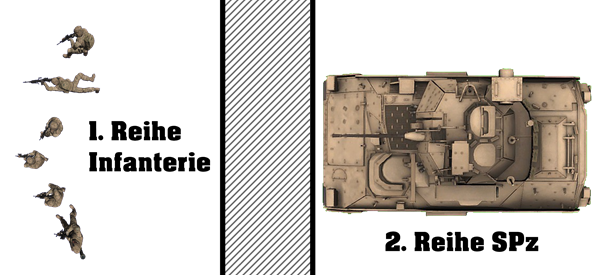
\includegraphics[width=0.95\linewidth]{./img/tutorials/spz/reihe}
		\caption{Sicherungspostionen Infanterie und SPz}
	\end{figure}

\section{Der Kampfpanzer}
	Der Kampfpanzer (kurz KPz) ist ein schwer gepanzertes Fahrzeug, welches primär zur Bekämpfung von harten Zielen eingesetzt wird, jedoch ebenso bestens für eine Bekämpfung weichen / halb-harten Zielen geeignet ist.\\

	In Arma 3 stehen viele verschiedene Modelle eines KPz zur Verfügung, welche sich in Bewaffnung / Visierung / Panzerung unterscheiden.\\
	In der folgenden Übersicht werden verschiedene Modelle mit ihren jeweiligen Spezifikationen aufgelistet.\\

\subsection{Modfahrzeuge}
\subsection{Vanilla Arma 3 Fahrzeuge}

\section{Bewaffnung und Panzerung von Kampfpanzer}
\subsection{Bewaffnung}
	Alle Kampfpanzer in Arma 3 sind mit einer Glattrohrkanone und einem leichten bis schweren Maschinengewehr ausgerüstet. Die Glattrohrkanone kann wahlweise mit einem HE- (High Explosive) oder einem AP- (Armor Piercing) Geschoss geladen werden.
	\begin{longtable}{ll} 
		\toprule
		Waffensystem & Zieltyp\\
		\midrule
		\multirow{3}{*}{Glattrohrkanone} & Weich (HE)\\
		& Halb-Hart (AP)\\
		& Hart (AP)\\
		Maschinengewehr (Koaxial) & Weich\\
		\bottomrule 
	\end{longtable}

\subsection{Panzerung}
	Die Hauptpanzerung des Fahrzeuges bietet vollständigen Schutz gegenüber Beschuss von Handfeuerwaffen. Potentielle Gegner des Kampfpanzers stellen schwere Feindkräfte wie Jets, Helikopter, SPz, KPz und spezialisierte Infanterietruppen dar. Diese können, bedingt durch ihre spezialisierten Anti-Panzer-Bewaffnungen, immensen Schaden am Fahrzeug ausrichten, bis hin zum Totalverlust des Fahrzeuges. 

\section{Die Crew}
\label{sec:panzercrew}
	Die Crew ist das wichtigste Element eines Panzerfahrzeuges und bildet somit das Herzstück dieser Einheit. Nur eine eingespielte Besatzung kann das Fahrzeug effektiv einsetzen und so das Kampfgeschehen im entscheidenden Moment beherrschen.\\
	Hierbei ist die Kommunikation der wichtigste Faktor und sollte nicht unterschätzt werden, im Ernstfall entscheiden wenige Sekunden über Leben und Tod der Besatzung.\\

	Eine erfolgreich eingespielte Crew zeichnet sich dadurch aus, dass in der Kampfphase nurnoch wenige Worte gesprochen werden müssen, da eine Vielzahl der nötigen Befehle bereits in einen Automatismus übergegangen sind. Gegenseitiges, uneingeschränktes Vertrauen in die jeweils anderen ist hier unumgänglich.\\

	Jedem Posten innerhalb des Panzerfahrzeuges sind spezielle Aufgaben zugewiesen, welche in der folgenden Tabelle näher erläutert werden.

\subsection{Die Aufgaben der Crew}
	\begin{longtable}{lp{0.5\textwidth}} 
		\toprule
		\multirow{2}{*}{Kommandant} & Zentrales Führungselement des Fahrzeuges\\
		& \begin{minipage}[t]{0.4\textwidth}
			Aufgaben:
			\begin{itemize}
				\item Führen des Panzerfahrzeuges
				\item Oberbefehl über die Infanterie
				\item Gesamtüberblick behalten
				\item Kommunikation mit anderen Einheiten
			\end{itemize}
		\end{minipage}\\
		\midrule
		\multirow{2}{*}{Richtschütze} & Bedienung der Waffenanlage\\
		& \begin{minipage}[t]{0.4\textwidth}
			Aufgaben:
			\begin{itemize}
				\item Bedienung der Waffenanlage
				\item Überwachung der Umgebung
				\item Feindkontakt melden
				\item Einweisen des Fahrers
			\end{itemize}
		\end{minipage}\\	
		\midrule
		\multirow{2}{*}{Kraftfahrer} & Steuerung des Fahrzeuges\\
		& \begin{minipage}[t]{0.4\textwidth}
			Aufgaben:
			\begin{itemize}
				\item Sicheres Manövrieren des Fahrzeuges
				\item Ausführen der Befehle
				\item Feindkontakt melden
			\end{itemize}
		\end{minipage}\\		
		\bottomrule 
	\end{longtable}
	
\section{Steuerung und Befehle}
	In diesem Kapitel wird anhand von Beispielen die Steuerung- und Befehlsstruktur zur Führung eines Panzerfahrzeuges erklärt.
	
\subsection{Fahrer: Steuerung, Befehle und Hinweise}
\subsubsection{Steuerung}
	\begin{longtable}{ll} 
		\toprule
		Steuerung & Tasten\\
		\midrule
		Fahrzeug steuern & \keys{W}, \keys{A}, \keys{S}, \keys{D}\\
		Schnell fahren & \keys{Shift + W}\\
		Langsam fahren & \keys{Strg + W}\\
		Luke auf\,/\,Luke zu & \keys{Strg + Q}\,/\,\keys{Strg + E}\\
		Handbremse (nur bei Radfahrzeugen) & \keys{X}\\
		Geschwindigkeitsbegrenzer an\,/\,aus & \keys{Entf}\\
				\bottomrule 
	\end{longtable}	
	
\subsubsection{Befehle}
	Wie bereits in Kapitel \ref{sec:panzercrew} \nameref{sec:panzercrew} angemerkt, ist die Kommunikation im Fahrzeug äußerst wichtig. Deshalb beschränkt sich die Kommunikation zwischen Kommandant und Fahrer auf kurze, prägnante Befehle, wie es den folgenden Beispielen zu entnehmen ist.

	\begin{longtable}{p{0.45\textwidth}p{0.5\textwidth}} 
		\toprule
		Kommando & Ausführung\\
		\midrule
		„Crew  Befehl  Hinweis“ & Die Kommandos sind modular aufgebaut und können entsprechend, je nach Situation, abgeändert werden.\\
		\midrule
		Den Panzer auf der Stelle (stehend) ausrichten (drehen).\vspace{6pt}\nl
		„Fahrer ausrichten 1-1-0 Grad“
		& Fahrer dreht die Panzerwanne in Kompassrichtung 1-1-0 Grad\\
		\midrule
		Den Panzer mit Richtgeschwindigkeit in Bewegung setzen.\vspace{6pt}\nl
		Fahrer vorwärts 2-2-0 Grad, 30 Km/h“
		& Kommando “Vorwärts” wird genutzt, um individuelle Geschwindigkeiten vorzugeben.\\
		\midrule
		Den Panzer in Bewegung setzen.\vspace{6pt}\nl
		„Fahrer Marsch 2-2-0 Grad“
		& Fahrer fährt mit verminderter Geschwindigkeit nach vorne (Strg + W), in Kompassrichtung 2-2-0 Grad.\\
		\midrule
		Den Panzer schnell in Bewegung setzen.\vspace{6pt}\nl
		„Fahrer  Marsch Marsch 2-2-0 Grad“
		& Fahrer fährt in normaler Geschwindigkeit (W) in Richtung 2-2-0 Grad\\
		\midrule
		Den Panzer schnellst möglich fahren.\vspace{6pt}\nl
		„Fahrer Sprung 2-2-0 Grad, Straße folgen.
		& Fahrer fährt mit Höchstgeschwindigkeit (Shift+W) in Richtung 2-2-0 Grad, und folgt der Straße.\\
		\midrule
		Den Panzer anhalten\vspace{6pt}\nl
		„Fahrer anhalten“
		& Der Fahrer bremst seinen Panzer sanft bis zum Stillstand.\\
		\midrule
		Den Panzer sofort zum stehen bringen.\vspace{6pt}\nl
		„Fahrer STOP“
		& Der Fahrer führt eine Vollbremsung aus. (Im Konvoi wegen hoher Unfallgefahr vermeiden)\\		 
		\bottomrule 
	\end{longtable}	
%\chapter{Tutorials}
%\section{Task Force Arrowhead Radio (TFAR)}
\label{TFAR}
\subsection{Tastaturkürzel}
\begin{longtable}{|p{2cm}|p{5 cm}||p{2cm}|p{4cm}|} 
	\caption[Trupp]{die wichtigsten Tasten TFAR Tasten} \\ 
	\hline
	\cellcolor{backcolor} \textbf{Taste} & \textbf{Beschreibung} & \cellcolor{backcolor}\textbf{Taste} & \textbf{Beschreibung}  \\ 
	\hline
	\cellcolor{backcolor} STRG + P & SR Funkgerät öffnen & \cellcolor{backcolor}  ALT + P &  LR Funkgerät öffnen \\
	\hline
	\cellcolor{backcolor} PTT im TS\footnote{Push to Talk bzw. Spracherkennung im Teamspeak} & direkt sprechen & \cellcolor{backcolor}  Caps Lock & Auf SR Funk funken \\
	 \hline
	\cellcolor{backcolor} T & Aud SR Additional Channel funken & \cellcolor{backcolor}  Y & Auf LR Additional Channel funken \\
	 \hline
	\cellcolor{backcolor} STRG + TAB & Gesprächslautstärke einstellen\footnote{whispering / normal / yelling} & \cellcolor{backcolor}  & \\
	 \hline
	\cellcolor{backcolor} SHIFT + P & Unterwasserfunkgerät & \cellcolor{backcolor}  STRG + \~ & Auf Unterwasserfunk funken \\
	 \hline
\end{longtable}
\subsection{Short Range Funkgerät (AN/PRC – 152)}
	\begin{minipage} [b]{0.5\textwidth}
		\begin{enumerate}
			\item Lautstärke einstellen
			\item aktueller Kanal
			\item aktuelle Funkfrequenz
			\item Stereo Einstellungen\nl (linkes Ohr / rechtes Ohr)
			\item Funkfrequenz festlegen
			\item Frequenz löschen
			\item Frequenz bestätigen
			\item Funkkanal wechseln
			\item Umschaltung zwischen\nl Lautsprecher -- Kopfhörer
			\item Additional Channel festlegen
		\end{enumerate}
	\end{minipage}
	\begin{minipage}[t]{0.4\textwidth}
		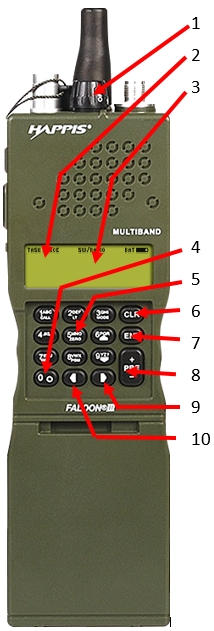
\includegraphics[width=\textwidth]{./img/tutorials/tfar/TFAR_SR_Radio.png}
	\end{minipage}


\subsection{Long Range Funkgerät (RT-15236 (ASIP) - LR)}
\begin{minipage}[t]{1\textwidth}
	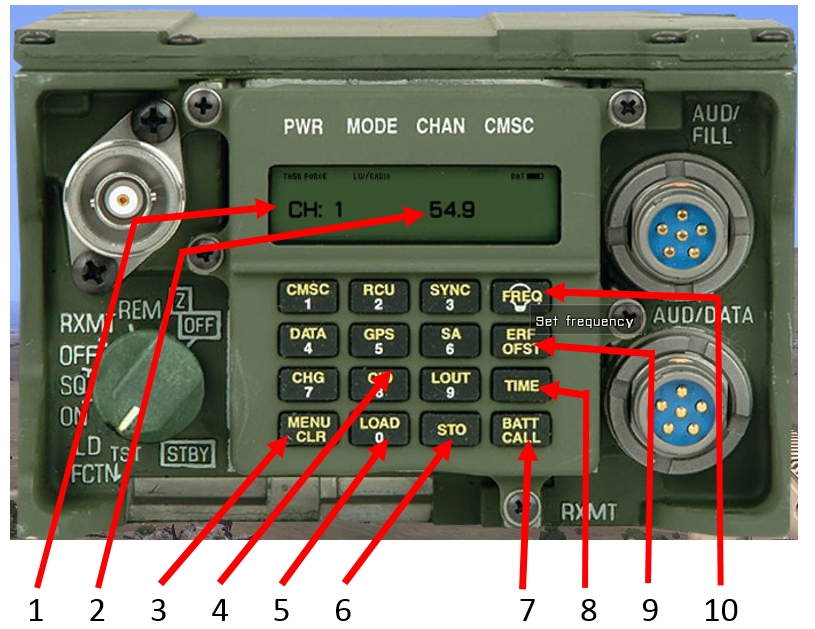
\includegraphics[width=\textwidth]{./img/tutorials/tfar/TFAR_LR_Radio.png}
\end{minipage}
\begin{enumerate}
	\item aktueller Kanal
	\item aktuelle Funkfrequenz
	\item Frequenz löschen
	\item Tastenfeld zur Eingabe der Funkfrequenz
	\item umschalten zwischen Lautsprecher und Kopfhörer
	\item Stereo Einstellungen (linkes Ohr / rechtes Ohr)
	\item Lautstärke  senken
	\item Lautstärke erhöhen
	\item Additional Channel festlegen
	\item Frequenz bestätigen
\end{enumerate}

%\pagebreak

%Sonstiges
%\chapter{Sonstiges}
%%\begin{landscape} %Querformat
\section{nützliche Tastatur (Um)Belegung}
Tipp: Kompass auf >>Leertaste<< legen so ist dieser leichter verfügbar als über die Taste >>K<<
%\end{landscape}
%das Abkürzungsverzeichnis erstellen
\pagebreak
\chapter*{Abkürzungsverzeichnis}
\addcontentsline{toc}{chapter}{Abk\"urzungsverzeichnis} 
\begin{acronym}[SEPSEPSEP]
\setlength{\itemsep}{1em}
	\acro{AAR}{After Action Report}
	\acro{OPL}{Operationsleitung}
	\acro{SQL}{Squadlead}
	\acro{FAC}{Forward Air Controler}
	\acro{AT}{Anti Tank}
	\acro{UAV}{Unmanned Aerial Vehicle}
	\acro{TTT}{Tactical Training Team}
	\acro{AA}{Anti Air}
	\acro{KPZ}{Kampfpanzer}	
	\acro{SPZ}{Schützenpanzer}
	\acro{CAS}{Close Air Support}
	\acro{CQB}{Operationsleitung}
	\acro{AGA}{Allgemeine Grundausbildung}
	\acro{SGA}{Spezielle Grundausbildung}
	\acro{KSK}{Kommando Spezialkräfte}
	\acro{MedEvac}{MEDical EVACuation}
	\acro{CSE}{Combat Space Enhancement}
	\acro{IR}{Infrarot}
	\acro{EOD}{Explosive Ordnance Disposal}
	\acro{LZ}{Landezone}
	\acro{KT}{Kampftrupp}
	\acro{SR}{Short Range}
	\acro{LR}{Long Range}
	\acro{MG}{Maschinengewehr}
\end{acronym}
\pagebreak

%Ganz zum Schluss
\pagebreak
\chapter*{Autoren}
\addcontentsline{toc}{chapter}{Autoren} 
	Ein herzliches Dank an euch für eure fleißige Mitarbeit, sowie an alle die am \ac{TTT} mitwirken. 
	\par\bigskip
	\begin{tabular}{p{0.23\textwidth}p{0.23\textwidth}p{0.23\textwidth}p{0.23\textwidth}}
		Ghost & 
		grauer Wolf &
		Grunt &
		GSG9\_abzocker\\
		Highhead &
		LingLing & 
		Lorddrinkalot &
		Lufros\\
		Mynx &
		Nachti &
		Reimchen &
		Relain\\
		Schotte &
		SCiite &
		Speutzi &
		Stura \\
		TheConen\\
	\end{tabular}	

\cleardoublepage
\appendix
\end{document}